\section{Comparison of Importance Sampling method}
\label{sec:simulation_studies}

\begin{example}[univariate Gaussian, $\sigma^{2}$ fixed]
    \label{ex:univ-gaussian-s2-fixed}
    Consider the probability space $ \left( \R, \mathcal B(\R), \P \right)$ where $\P = p\lambda$ for the Lebesgue measure $\lambda$ which is symmetric around $0$, i.e. $p(-x) = p(x)$ for $\lambda$-a.e. $x\in\R$ and possesses up to third order moments.
    Let $\G=\P$, so $W\equiv1$ and let $\G_{\psi} = \mathcal N \left( \sigma\psi, \sigma^{2} \right)$ be the single parameter natural exponential family of Gaussians with fixed variance $\sigma^{2} > 0$. Then 
    $$
    \log g_{\psi}(x) = \psi T(x) - \frac{\psi^{2}}{2} + \log h(x),
    $$
    where $T(x) = \frac{x}{\sigma}$ and $h(x)$ is the density of $\mathcal N(0, \sigma^{2})$ w.r.t. Lebesgue measure. 
    Note that $T$ is centered under $\P$. To compare the asymptotic behavior of the \gls{cem} and \gls{eis} we compute the asymptotic variances arising from their respective central limit theorems (\Cref{thm:ce-clt,thm:clt-eis}).

    By symmetry, both $\pce$ and $\peis$ are equal to $0$. 
    Then $I(\psi) = 1$ for all $\psi$, so 
    \begin{align}
    \label{eq:ce-gaussian-mean-var}
        V_{\ce} = \cov_{\P}(T) = \frac{\tau^{2}}{\sigma^{2}},
    \end{align}
    where $\tau^{2}=\P \operatorname{id}^{2}$ is the second moment of $\P$. 
    Additionally, $B_{\eis} = (\cov_{\P}(T))^{-1} = \frac{\sigma^{2}}{\tau^{2}}$ and
    \begin{align*}
    M_{\eis} &= \cov_{\P} \left( (\log \frac{p(x)}{h(x)} - \lambda_{\eis})T\right) \\
        &= \cov_{\P} \left(\left( \log p - \log h - \P (\log p - \log h) \right) T \right) \\
        &= \frac{1}{\sigma^{2}}\int p(x) x^{2}\left(\log p(x) + \frac{x^{2}}{2\sigma^{2}} - \P\left(\log p(x) + \frac{\tau^{2}}{2\sigma^{2}}\right)\right)^{2} \d x.
    \end{align*}
    Thus
    $$
    V_{\eis} = B_{\eis}M_{\eis}B_{\eis}= \sigma^{2}\frac{\gamma}{\tau^{4}},
    $$
    where $\gamma = \int p(x) x^{2}\left(\log p(x) + \frac{x^{2}}{2\sigma^{2}} - \P(\log p(x) + \frac{\tau^{2}}{2\sigma^{2}})\right)^{2} \d x.$
    
    \paragraph{Normal distribution}
    If $\P = \mathcal N(0, \tau^{2})$ is a normal distribution, this reduces to
    \begin{align*}
        V_{\eis} &= \frac{5}{2} \left( \frac{\tau^{2}}{\sigma^{2}} - 1 \right)^{2} \frac{\sigma^{2}}{\tau^{2}} = \frac{5}{2} \frac{\left( V_{\ce} - 1\right)^{2}}{V_{\ce}}
    \end{align*}
    and so for $\tau^{2} = \sigma^{2}$ $\hpeis$ converges faster than the standard $\mathcal O( N^{-\frac{1}{2}})$ rate. Indeed in this case $\hpeis = \peis$ a.s. for $N > 1$ see \todo{write example for EIS being exact for exponential families}. 

    For importance sampling to be consistent, it is necessary that $\sigma^{2} > \frac{\tau^{2}}{2}$. The left-hand side of \Cref{fig:normal_are} displays the behavior of the relative efficiency
    $$
    \frac{V_{\eis}}{V_{\ce}} = \frac{5}{2} \frac{(V_{\ce} - 1)^{2}}{V_{\ce}^{2}} = \frac{5}{2} \left( 1 - \frac{2}{Vsdf_{\ce}} + \frac{1}{V_{\ce}^2} \right)
    $$

    \begin{figure}
        \centering

        \begin{subfigure}{.49\textwidth}
            \resizebox{\textwidth}{!}{%
                % Created by tikzDevice version 0.12.6 on 2024-06-05 16:48:21
% !TEX encoding = UTF-8 Unicode
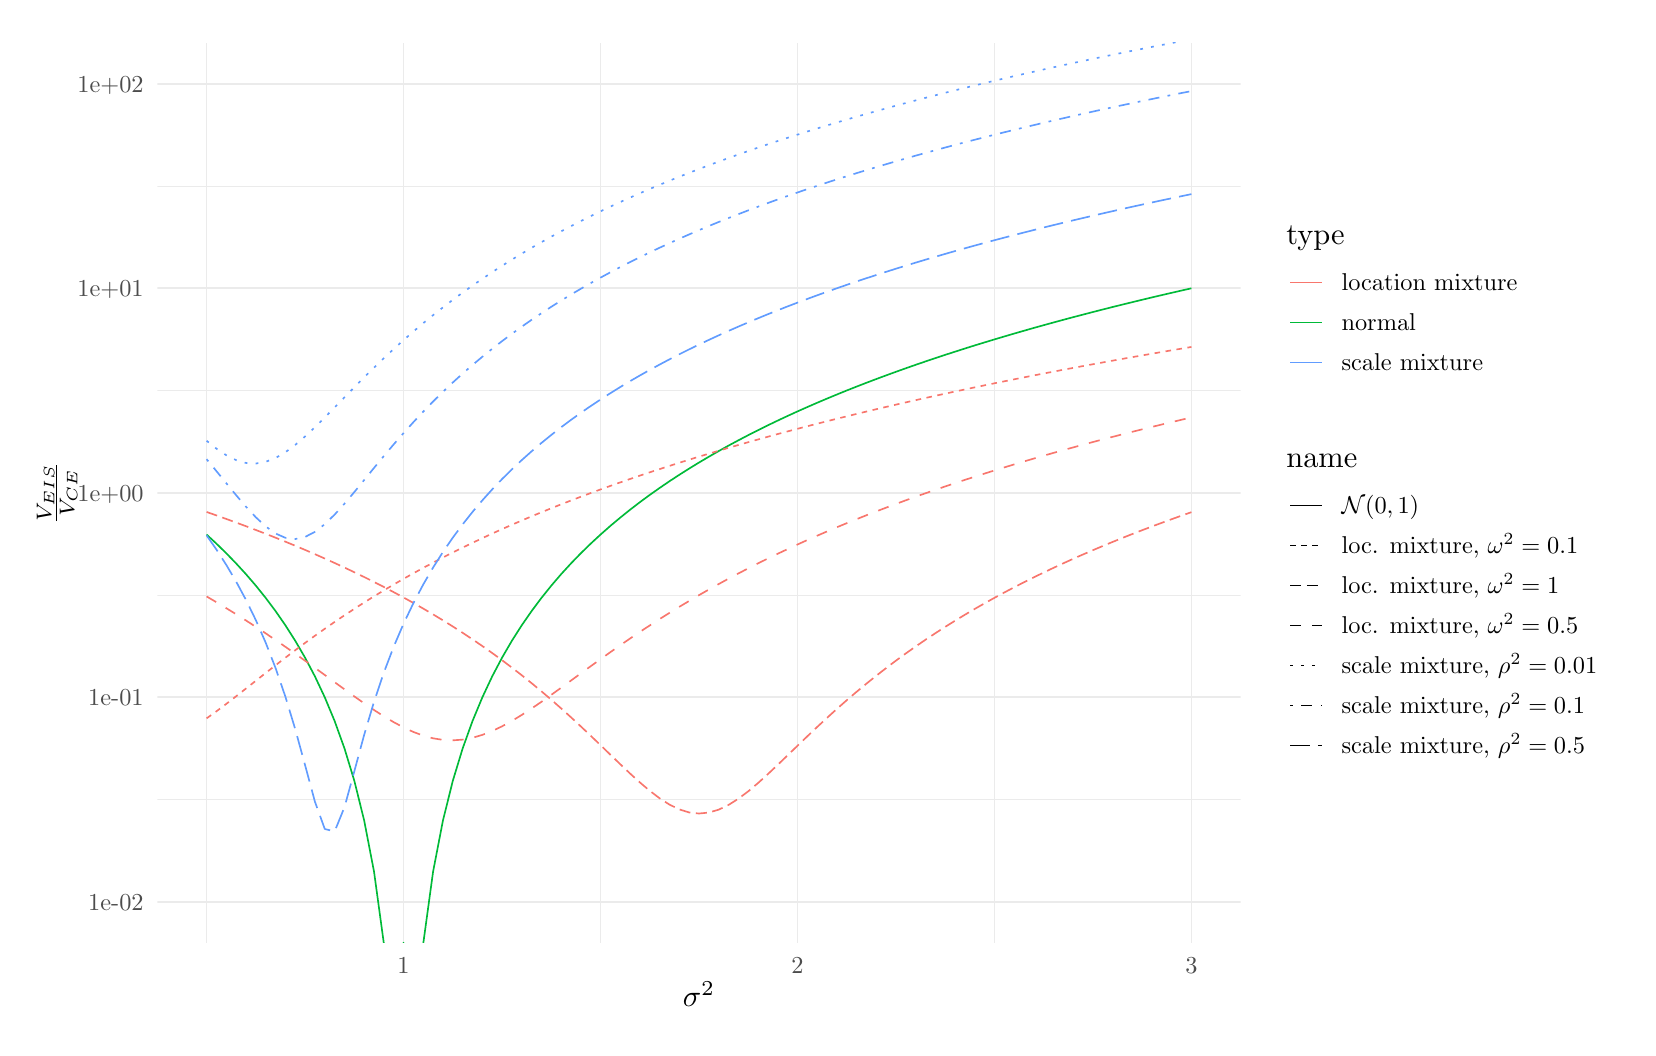
\begin{tikzpicture}[x=1pt,y=1pt]
\definecolor{fillColor}{RGB}{255,255,255}
\path[use as bounding box,fill=fillColor,fill opacity=0.00] (0,0) rectangle (578.16,361.35);
\begin{scope}
\path[clip] ( 46.86, 30.69) rectangle (438.30,355.85);
\definecolor{drawColor}{gray}{0.92}

\path[draw=drawColor,line width= 0.3pt,line join=round] ( 46.86, 82.42) --
	(438.30, 82.42);

\path[draw=drawColor,line width= 0.3pt,line join=round] ( 46.86,156.32) --
	(438.30,156.32);

\path[draw=drawColor,line width= 0.3pt,line join=round] ( 46.86,230.22) --
	(438.30,230.22);

\path[draw=drawColor,line width= 0.3pt,line join=round] ( 46.86,304.12) --
	(438.30,304.12);

\path[draw=drawColor,line width= 0.3pt,line join=round] ( 64.66, 30.69) --
	( 64.66,355.85);

\path[draw=drawColor,line width= 0.3pt,line join=round] (207.00, 30.69) --
	(207.00,355.85);

\path[draw=drawColor,line width= 0.3pt,line join=round] (349.34, 30.69) --
	(349.34,355.85);

\path[draw=drawColor,line width= 0.6pt,line join=round] ( 46.86, 45.47) --
	(438.30, 45.47);

\path[draw=drawColor,line width= 0.6pt,line join=round] ( 46.86,119.37) --
	(438.30,119.37);

\path[draw=drawColor,line width= 0.6pt,line join=round] ( 46.86,193.27) --
	(438.30,193.27);

\path[draw=drawColor,line width= 0.6pt,line join=round] ( 46.86,267.17) --
	(438.30,267.17);

\path[draw=drawColor,line width= 0.6pt,line join=round] ( 46.86,341.07) --
	(438.30,341.07);

\path[draw=drawColor,line width= 0.6pt,line join=round] (135.83, 30.69) --
	(135.83,355.85);

\path[draw=drawColor,line width= 0.6pt,line join=round] (278.17, 30.69) --
	(278.17,355.85);

\path[draw=drawColor,line width= 0.6pt,line join=round] (420.51, 30.69) --
	(420.51,355.85);
\definecolor{drawColor}{RGB}{0,186,56}

\path[draw=drawColor,line width= 0.6pt,line join=round] ( 64.66,178.18) --
	( 68.22,174.89) --
	( 71.77,171.42) --
	( 75.33,167.75) --
	( 78.89,163.86) --
	( 82.45,159.72) --
	( 86.01,155.29) --
	( 89.57,150.53) --
	( 93.13,145.39) --
	( 96.68,139.81) --
	(100.24,133.69) --
	(103.80,126.93) --
	(107.36,119.37) --
	(110.92,110.80) --
	(114.48,100.90) --
	(118.04, 89.20) --
	(121.59, 74.87) --
	(125.15, 56.41) --
	(128.71, 30.38) --
	(132.27,-14.11) --
	(135.83, 30.69) --
	(139.39,-14.11) --
	(142.94, 30.38) --
	(146.50, 56.41) --
	(150.06, 74.87) --
	(153.62, 89.20) --
	(157.18,100.90) --
	(160.74,110.80) --
	(164.30,119.37) --
	(167.85,126.93) --
	(171.41,133.69) --
	(174.97,139.81) --
	(178.53,145.39) --
	(182.09,150.53) --
	(185.65,155.29) --
	(189.21,159.72) --
	(192.76,163.86) --
	(196.32,167.75) --
	(199.88,171.42) --
	(203.44,174.89) --
	(207.00,178.18) --
	(210.56,181.32) --
	(214.12,184.30) --
	(217.67,187.15) --
	(221.23,189.89) --
	(224.79,192.51) --
	(228.35,195.02) --
	(231.91,197.45) --
	(235.47,199.78) --
	(239.03,202.03) --
	(242.58,204.21) --
	(246.14,206.31) --
	(249.70,208.35) --
	(253.26,210.33) --
	(256.82,212.24) --
	(260.38,214.10) --
	(263.94,215.91) --
	(267.49,217.67) --
	(271.05,219.38) --
	(274.61,221.05) --
	(278.17,222.68) --
	(281.73,224.26) --
	(285.29,225.81) --
	(288.85,227.32) --
	(292.40,228.79) --
	(295.96,230.24) --
	(299.52,231.65) --
	(303.08,233.03) --
	(306.64,234.38) --
	(310.20,235.70) --
	(313.75,237.00) --
	(317.31,238.27) --
	(320.87,239.52) --
	(324.43,240.74) --
	(327.99,241.94) --
	(331.55,243.12) --
	(335.11,244.27) --
	(338.66,245.41) --
	(342.22,246.53) --
	(345.78,247.62) --
	(349.34,248.70) --
	(352.90,249.76) --
	(356.46,250.81) --
	(360.02,251.83) --
	(363.57,252.85) --
	(367.13,253.84) --
	(370.69,254.82) --
	(374.25,255.79) --
	(377.81,256.74) --
	(381.37,257.67) --
	(384.93,258.60) --
	(388.48,259.51) --
	(392.04,260.41) --
	(395.60,261.29) --
	(399.16,262.16) --
	(402.72,263.03) --
	(406.28,263.88) --
	(409.84,264.72) --
	(413.39,265.54) --
	(416.95,266.36) --
	(420.51,267.17);
\definecolor{drawColor}{RGB}{248,118,109}

\path[draw=drawColor,line width= 0.6pt,dash pattern=on 2pt off 2pt ,line join=round] ( 64.66,111.77) --
	( 68.22,114.32) --
	( 71.77,117.00) --
	( 75.33,119.75) --
	( 78.89,122.55) --
	( 82.45,125.36) --
	( 86.01,128.17) --
	( 89.57,130.95) --
	( 93.13,133.69) --
	( 96.68,136.39) --
	(100.24,139.03) --
	(103.80,141.62) --
	(107.36,144.14) --
	(110.92,146.61) --
	(114.48,149.01) --
	(118.04,151.35) --
	(121.59,153.64) --
	(125.15,155.86) --
	(128.71,158.02) --
	(132.27,160.13) --
	(135.83,162.19) --
	(139.39,164.19) --
	(142.94,166.14) --
	(146.50,168.04) --
	(150.06,169.90) --
	(153.62,171.71) --
	(157.18,173.48) --
	(160.74,175.20) --
	(164.30,176.89) --
	(167.85,178.54) --
	(171.41,180.15) --
	(174.97,181.72) --
	(178.53,183.26) --
	(182.09,184.77) --
	(185.65,186.24) --
	(189.21,187.69) --
	(192.76,189.10) --
	(196.32,190.49) --
	(199.88,191.85) --
	(203.44,193.18) --
	(207.00,194.49) --
	(210.56,195.77) --
	(214.12,197.03) --
	(217.67,198.26) --
	(221.23,199.48) --
	(224.79,200.67) --
	(228.35,201.84) --
	(231.91,202.99) --
	(235.47,204.13) --
	(239.03,205.24) --
	(242.58,206.34) --
	(246.14,207.41) --
	(249.70,208.47) --
	(253.26,209.52) --
	(256.82,210.55) --
	(260.38,211.56) --
	(263.94,212.55) --
	(267.49,213.54) --
	(271.05,214.51) --
	(274.61,215.46) --
	(278.17,216.40) --
	(281.73,217.33) --
	(285.29,218.24) --
	(288.85,219.14) --
	(292.40,220.03) --
	(295.96,220.91) --
	(299.52,221.78) --
	(303.08,222.63) --
	(306.64,223.48) --
	(310.20,224.31) --
	(313.75,225.13) --
	(317.31,225.95) --
	(320.87,226.75) --
	(324.43,227.54) --
	(327.99,228.33) --
	(331.55,229.10) --
	(335.11,229.87) --
	(338.66,230.62) --
	(342.22,231.37) --
	(345.78,232.11) --
	(349.34,232.84) --
	(352.90,233.56) --
	(356.46,234.28) --
	(360.02,234.99) --
	(363.57,235.69) --
	(367.13,236.38) --
	(370.69,237.06) --
	(374.25,237.74) --
	(377.81,238.41) --
	(381.37,239.08) --
	(384.93,239.73) --
	(388.48,240.38) --
	(392.04,241.03) --
	(395.60,241.67) --
	(399.16,242.30) --
	(402.72,242.92) --
	(406.28,243.54) --
	(409.84,244.16) --
	(413.39,244.77) --
	(416.95,245.37) --
	(420.51,245.97);

\path[draw=drawColor,line width= 0.6pt,dash pattern=on 4pt off 2pt ,line join=round] ( 64.66,186.35) --
	( 68.22,185.10) --
	( 71.77,183.82) --
	( 75.33,182.52) --
	( 78.89,181.20) --
	( 82.45,179.84) --
	( 86.01,178.46) --
	( 89.57,177.05) --
	( 93.13,175.61) --
	( 96.68,174.14) --
	(100.24,172.64) --
	(103.80,171.10) --
	(107.36,169.52) --
	(110.92,167.91) --
	(114.48,166.26) --
	(118.04,164.57) --
	(121.59,162.84) --
	(125.15,161.06) --
	(128.71,159.24) --
	(132.27,157.37) --
	(135.83,155.44) --
	(139.39,153.47) --
	(142.94,151.43) --
	(146.50,149.34) --
	(150.06,147.19) --
	(153.62,144.97) --
	(157.18,142.68) --
	(160.74,140.32) --
	(164.30,137.89) --
	(167.85,135.38) --
	(171.41,132.79) --
	(174.97,130.11) --
	(178.53,127.35) --
	(182.09,124.49) --
	(185.65,121.54) --
	(189.21,118.50) --
	(192.76,115.37) --
	(196.32,112.16) --
	(199.88,108.86) --
	(203.44,105.49) --
	(207.00,102.08) --
	(210.56, 98.63) --
	(214.12, 95.21) --
	(217.67, 91.84) --
	(221.23, 88.61) --
	(224.79, 85.59) --
	(228.35, 82.89) --
	(231.91, 80.61) --
	(235.47, 78.87) --
	(239.03, 77.77) --
	(242.58, 77.38) --
	(246.14, 77.73) --
	(249.70, 78.78) --
	(253.26, 80.49) --
	(256.82, 82.73) --
	(260.38, 85.41) --
	(263.94, 88.42) --
	(267.49, 91.64) --
	(271.05, 95.00) --
	(274.61, 98.42) --
	(278.17,101.87) --
	(281.73,105.29) --
	(285.29,108.66) --
	(288.85,111.96) --
	(292.40,115.18) --
	(295.96,118.32) --
	(299.52,121.36) --
	(303.08,124.31) --
	(306.64,127.17) --
	(310.20,129.94) --
	(313.75,132.63) --
	(317.31,135.22) --
	(320.87,137.74) --
	(324.43,140.18) --
	(327.99,142.54) --
	(331.55,144.83) --
	(335.11,147.05) --
	(338.66,149.21) --
	(342.22,151.31) --
	(345.78,153.34) --
	(349.34,155.32) --
	(352.90,157.25) --
	(356.46,159.13) --
	(360.02,160.95) --
	(363.57,162.73) --
	(367.13,164.47) --
	(370.69,166.16) --
	(374.25,167.81) --
	(377.81,169.43) --
	(381.37,171.00) --
	(384.93,172.54) --
	(388.48,174.05) --
	(392.04,175.52) --
	(395.60,176.97) --
	(399.16,178.38) --
	(402.72,179.76) --
	(406.28,181.11) --
	(409.84,182.44) --
	(413.39,183.74) --
	(416.95,185.02) --
	(420.51,186.27);

\path[draw=drawColor,line width= 0.6pt,dash pattern=on 4pt off 4pt ,line join=round] ( 64.66,155.82) --
	( 68.22,153.73) --
	( 71.77,151.58) --
	( 75.33,149.39) --
	( 78.89,147.14) --
	( 82.45,144.83) --
	( 86.01,142.48) --
	( 89.57,140.08) --
	( 93.13,137.62) --
	( 96.68,135.13) --
	(100.24,132.59) --
	(103.80,130.03) --
	(107.36,127.44) --
	(110.92,124.84) --
	(114.48,122.26) --
	(118.04,119.70) --
	(121.59,117.20) --
	(125.15,114.79) --
	(128.71,112.50) --
	(132.27,110.39) --
	(135.83,108.49) --
	(139.39,106.85) --
	(142.94,105.53) --
	(146.50,104.56) --
	(150.06,103.99) --
	(153.62,103.83) --
	(157.18,104.08) --
	(160.74,104.75) --
	(164.30,105.80) --
	(167.85,107.19) --
	(171.41,108.89) --
	(174.97,110.84) --
	(178.53,113.00) --
	(182.09,115.32) --
	(185.65,117.75) --
	(189.21,120.27) --
	(192.76,122.83) --
	(196.32,125.42) --
	(199.88,128.02) --
	(203.44,130.60) --
	(207.00,133.16) --
	(210.56,135.69) --
	(214.12,138.18) --
	(217.67,140.62) --
	(221.23,143.01) --
	(224.79,145.35) --
	(228.35,147.65) --
	(231.91,149.88) --
	(235.47,152.07) --
	(239.03,154.20) --
	(242.58,156.29) --
	(246.14,158.32) --
	(249.70,160.30) --
	(253.26,162.24) --
	(256.82,164.13) --
	(260.38,165.98) --
	(263.94,167.78) --
	(267.49,169.54) --
	(271.05,171.26) --
	(274.61,172.94) --
	(278.17,174.59) --
	(281.73,176.20) --
	(285.29,177.77) --
	(288.85,179.31) --
	(292.40,180.82) --
	(295.96,182.30) --
	(299.52,183.74) --
	(303.08,185.16) --
	(306.64,186.55) --
	(310.20,187.91) --
	(313.75,189.25) --
	(317.31,190.56) --
	(320.87,191.85) --
	(324.43,193.11) --
	(327.99,194.35) --
	(331.55,195.57) --
	(335.11,196.76) --
	(338.66,197.94) --
	(342.22,199.10) --
	(345.78,200.23) --
	(349.34,201.35) --
	(352.90,202.45) --
	(356.46,203.53) --
	(360.02,204.60) --
	(363.57,205.65) --
	(367.13,206.68) --
	(370.69,207.70) --
	(374.25,208.70) --
	(377.81,209.68) --
	(381.37,210.66) --
	(384.93,211.62) --
	(388.48,212.56) --
	(392.04,213.49) --
	(395.60,214.41) --
	(399.16,215.32) --
	(402.72,216.21) --
	(406.28,217.09) --
	(409.84,217.96) --
	(413.39,218.82) --
	(416.95,219.67) --
	(420.51,220.51);
\definecolor{drawColor}{RGB}{97,156,255}

\path[draw=drawColor,line width= 0.6pt,dash pattern=on 1pt off 3pt ,line join=round] ( 64.66,212.08) --
	( 68.22,209.22) --
	( 71.77,206.84) --
	( 75.33,205.08) --
	( 78.89,204.06) --
	( 82.45,203.85) --
	( 86.01,204.47) --
	( 89.57,205.86) --
	( 93.13,207.94) --
	( 96.68,210.57) --
	(100.24,213.63) --
	(103.80,216.97) --
	(107.36,220.50) --
	(110.92,224.13) --
	(114.48,227.78) --
	(118.04,231.42) --
	(121.59,235.00) --
	(125.15,238.50) --
	(128.71,241.92) --
	(132.27,245.24) --
	(135.83,248.45) --
	(139.39,251.56) --
	(142.94,254.57) --
	(146.50,257.47) --
	(150.06,260.28) --
	(153.62,263.00) --
	(157.18,265.62) --
	(160.74,268.16) --
	(164.30,270.61) --
	(167.85,272.99) --
	(171.41,275.30) --
	(174.97,277.53) --
	(178.53,279.70) --
	(182.09,281.80) --
	(185.65,283.84) --
	(189.21,285.83) --
	(192.76,287.76) --
	(196.32,289.64) --
	(199.88,291.47) --
	(203.44,293.25) --
	(207.00,294.98) --
	(210.56,296.68) --
	(214.12,298.33) --
	(217.67,299.94) --
	(221.23,301.52) --
	(224.79,303.06) --
	(228.35,304.56) --
	(231.91,306.04) --
	(235.47,307.48) --
	(239.03,308.89) --
	(242.58,310.27) --
	(246.14,311.62) --
	(249.70,312.95) --
	(253.26,314.25) --
	(256.82,315.53) --
	(260.38,316.78) --
	(263.94,318.01) --
	(267.49,319.21) --
	(271.05,320.40) --
	(274.61,321.56) --
	(278.17,322.70) --
	(281.73,323.83) --
	(285.29,324.93) --
	(288.85,326.02) --
	(292.40,327.09) --
	(295.96,328.14) --
	(299.52,329.17) --
	(303.08,330.19) --
	(306.64,331.19) --
	(310.20,332.18) --
	(313.75,333.16) --
	(317.31,334.12) --
	(320.87,335.06) --
	(324.43,335.99) --
	(327.99,336.91) --
	(331.55,337.82) --
	(335.11,338.71) --
	(338.66,339.59) --
	(342.22,340.46) --
	(345.78,341.32) --
	(349.34,342.17) --
	(352.90,343.00) --
	(356.46,343.83) --
	(360.02,344.64) --
	(363.57,345.45) --
	(367.13,346.25) --
	(370.69,347.03) --
	(374.25,347.81) --
	(377.81,348.57) --
	(381.37,349.33) --
	(384.93,350.08) --
	(388.48,350.82) --
	(392.04,351.56) --
	(395.60,352.28) --
	(399.16,353.00) --
	(402.72,353.70) --
	(406.28,354.41) --
	(409.84,355.10) --
	(413.39,355.78) --
	(416.95,356.46) --
	(420.51,357.14);

\path[draw=drawColor,line width= 0.6pt,dash pattern=on 1pt off 3pt on 4pt off 3pt ,line join=round] ( 64.66,205.42) --
	( 68.22,201.09) --
	( 71.77,196.73) --
	( 75.33,192.41) --
	( 78.89,188.25) --
	( 82.45,184.42) --
	( 86.01,181.12) --
	( 89.57,178.57) --
	( 93.13,177.01) --
	( 96.68,176.57) --
	(100.24,177.32) --
	(103.80,179.17) --
	(107.36,181.93) --
	(110.92,185.40) --
	(114.48,189.34) --
	(118.04,193.55) --
	(121.59,197.89) --
	(125.15,202.26) --
	(128.71,206.57) --
	(132.27,210.78) --
	(135.83,214.87) --
	(139.39,218.81) --
	(142.94,222.61) --
	(146.50,226.26) --
	(150.06,229.77) --
	(153.62,233.13) --
	(157.18,236.36) --
	(160.74,239.46) --
	(164.30,242.44) --
	(167.85,245.31) --
	(171.41,248.07) --
	(174.97,250.73) --
	(178.53,253.30) --
	(182.09,255.78) --
	(185.65,258.17) --
	(189.21,260.49) --
	(192.76,262.73) --
	(196.32,264.90) --
	(199.88,267.00) --
	(203.44,269.04) --
	(207.00,271.02) --
	(210.56,272.95) --
	(214.12,274.82) --
	(217.67,276.64) --
	(221.23,278.42) --
	(224.79,280.14) --
	(228.35,281.83) --
	(231.91,283.47) --
	(235.47,285.07) --
	(239.03,286.64) --
	(242.58,288.17) --
	(246.14,289.67) --
	(249.70,291.13) --
	(253.26,292.56) --
	(256.82,293.96) --
	(260.38,295.33) --
	(263.94,296.67) --
	(267.49,297.99) --
	(271.05,299.28) --
	(274.61,300.55) --
	(278.17,301.79) --
	(281.73,303.01) --
	(285.29,304.20) --
	(288.85,305.38) --
	(292.40,306.53) --
	(295.96,307.66) --
	(299.52,308.78) --
	(303.08,309.88) --
	(306.64,310.95) --
	(310.20,312.01) --
	(313.75,313.06) --
	(317.31,314.08) --
	(320.87,315.10) --
	(324.43,316.09) --
	(327.99,317.07) --
	(331.55,318.04) --
	(335.11,318.99) --
	(338.66,319.93) --
	(342.22,320.85) --
	(345.78,321.76) --
	(349.34,322.66) --
	(352.90,323.55) --
	(356.46,324.42) --
	(360.02,325.29) --
	(363.57,326.14) --
	(367.13,326.98) --
	(370.69,327.81) --
	(374.25,328.63) --
	(377.81,329.44) --
	(381.37,330.24) --
	(384.93,331.03) --
	(388.48,331.81) --
	(392.04,332.58) --
	(395.60,333.34) --
	(399.16,334.09) --
	(402.72,334.84) --
	(406.28,335.57) --
	(409.84,336.30) --
	(413.39,337.02) --
	(416.95,337.73) --
	(420.51,338.43);

\path[draw=drawColor,line width= 0.6pt,dash pattern=on 7pt off 3pt ,line join=round] ( 64.66,177.88) --
	( 68.22,172.76) --
	( 71.77,167.22) --
	( 75.33,161.19) --
	( 78.89,154.57) --
	( 82.45,147.26) --
	( 86.01,139.11) --
	( 89.57,129.95) --
	( 93.13,119.59) --
	( 96.68,107.86) --
	(100.24, 94.86) --
	(103.80, 81.65) --
	(107.36, 71.79) --
	(110.92, 70.91) --
	(114.48, 79.67) --
	(118.04, 92.66) --
	(121.59,105.81) --
	(125.15,117.76) --
	(128.71,128.34) --
	(132.27,137.68) --
	(135.83,145.99) --
	(139.39,153.42) --
	(142.94,160.15) --
	(146.50,166.27) --
	(150.06,171.89) --
	(153.62,177.07) --
	(157.18,181.87) --
	(160.74,186.36) --
	(164.30,190.55) --
	(167.85,194.50) --
	(171.41,198.22) --
	(174.97,201.74) --
	(178.53,205.08) --
	(182.09,208.26) --
	(185.65,211.29) --
	(189.21,214.18) --
	(192.76,216.96) --
	(196.32,219.61) --
	(199.88,222.17) --
	(203.44,224.62) --
	(207.00,226.99) --
	(210.56,229.27) --
	(214.12,231.48) --
	(217.67,233.61) --
	(221.23,235.67) --
	(224.79,237.67) --
	(228.35,239.61) --
	(231.91,241.50) --
	(235.47,243.33) --
	(239.03,245.11) --
	(242.58,246.84) --
	(246.14,248.52) --
	(249.70,250.17) --
	(253.26,251.77) --
	(256.82,253.33) --
	(260.38,254.86) --
	(263.94,256.35) --
	(267.49,257.81) --
	(271.05,259.23) --
	(274.61,260.63) --
	(278.17,261.99) --
	(281.73,263.33) --
	(285.29,264.64) --
	(288.85,265.92) --
	(292.40,267.18) --
	(295.96,268.41) --
	(299.52,269.62) --
	(303.08,270.81) --
	(306.64,271.98) --
	(310.20,273.12) --
	(313.75,274.25) --
	(317.31,275.35) --
	(320.87,276.44) --
	(324.43,277.51) --
	(327.99,278.56) --
	(331.55,279.60) --
	(335.11,280.62) --
	(338.66,281.62) --
	(342.22,282.61) --
	(345.78,283.58) --
	(349.34,284.54) --
	(352.90,285.48) --
	(356.46,286.41) --
	(360.02,287.33) --
	(363.57,288.23) --
	(367.13,289.13) --
	(370.69,290.01) --
	(374.25,290.87) --
	(377.81,291.73) --
	(381.37,292.57) --
	(384.93,293.41) --
	(388.48,294.23) --
	(392.04,295.04) --
	(395.60,295.85) --
	(399.16,296.64) --
	(402.72,297.42) --
	(406.28,298.19) --
	(409.84,298.96) --
	(413.39,299.71) --
	(416.95,300.46) --
	(420.51,301.20);
\end{scope}
\begin{scope}
\path[clip] (  0.00,  0.00) rectangle (578.16,361.35);
\definecolor{drawColor}{gray}{0.30}

\node[text=drawColor,anchor=base east,inner sep=0pt, outer sep=0pt, scale=  0.88] at ( 41.91, 42.44) {1e-02};

\node[text=drawColor,anchor=base east,inner sep=0pt, outer sep=0pt, scale=  0.88] at ( 41.91,116.34) {1e-01};

\node[text=drawColor,anchor=base east,inner sep=0pt, outer sep=0pt, scale=  0.88] at ( 41.91,190.24) {1e+00};

\node[text=drawColor,anchor=base east,inner sep=0pt, outer sep=0pt, scale=  0.88] at ( 41.91,264.14) {1e+01};

\node[text=drawColor,anchor=base east,inner sep=0pt, outer sep=0pt, scale=  0.88] at ( 41.91,338.04) {1e+02};
\end{scope}
\begin{scope}
\path[clip] (  0.00,  0.00) rectangle (578.16,361.35);
\definecolor{drawColor}{gray}{0.30}

\node[text=drawColor,anchor=base,inner sep=0pt, outer sep=0pt, scale=  0.88] at (135.83, 19.68) {1};

\node[text=drawColor,anchor=base,inner sep=0pt, outer sep=0pt, scale=  0.88] at (278.17, 19.68) {2};

\node[text=drawColor,anchor=base,inner sep=0pt, outer sep=0pt, scale=  0.88] at (420.51, 19.68) {3};
\end{scope}
\begin{scope}
\path[clip] (  0.00,  0.00) rectangle (578.16,361.35);
\definecolor{drawColor}{RGB}{0,0,0}

\node[text=drawColor,anchor=base,inner sep=0pt, outer sep=0pt, scale=  1.10] at (242.58,  7.64) {$\sigma^2$};
\end{scope}
\begin{scope}
\path[clip] (  0.00,  0.00) rectangle (578.16,361.35);
\definecolor{drawColor}{RGB}{0,0,0}

\node[text=drawColor,rotate= 90.00,anchor=base,inner sep=0pt, outer sep=0pt, scale=  1.10] at ( 13.08,193.27) {$\frac{V_{EIS}}{V_{CE}}$};
\end{scope}
\begin{scope}
\path[clip] (  0.00,  0.00) rectangle (578.16,361.35);
\definecolor{drawColor}{RGB}{0,0,0}

\node[text=drawColor,anchor=base west,inner sep=0pt, outer sep=0pt, scale=  1.10] at (454.80,283.11) {type};
\end{scope}
\begin{scope}
\path[clip] (  0.00,  0.00) rectangle (578.16,361.35);
\definecolor{drawColor}{RGB}{248,118,109}

\path[draw=drawColor,line width= 0.6pt,line join=round] (456.25,269.31) -- (467.81,269.31);
\end{scope}
\begin{scope}
\path[clip] (  0.00,  0.00) rectangle (578.16,361.35);
\definecolor{drawColor}{RGB}{0,186,56}

\path[draw=drawColor,line width= 0.6pt,line join=round] (456.25,254.86) -- (467.81,254.86);
\end{scope}
\begin{scope}
\path[clip] (  0.00,  0.00) rectangle (578.16,361.35);
\definecolor{drawColor}{RGB}{97,156,255}

\path[draw=drawColor,line width= 0.6pt,line join=round] (456.25,240.40) -- (467.81,240.40);
\end{scope}
\begin{scope}
\path[clip] (  0.00,  0.00) rectangle (578.16,361.35);
\definecolor{drawColor}{RGB}{0,0,0}

\node[text=drawColor,anchor=base west,inner sep=0pt, outer sep=0pt, scale=  0.88] at (474.76,266.28) {location mixture};
\end{scope}
\begin{scope}
\path[clip] (  0.00,  0.00) rectangle (578.16,361.35);
\definecolor{drawColor}{RGB}{0,0,0}

\node[text=drawColor,anchor=base west,inner sep=0pt, outer sep=0pt, scale=  0.88] at (474.76,251.83) {normal};
\end{scope}
\begin{scope}
\path[clip] (  0.00,  0.00) rectangle (578.16,361.35);
\definecolor{drawColor}{RGB}{0,0,0}

\node[text=drawColor,anchor=base west,inner sep=0pt, outer sep=0pt, scale=  0.88] at (474.76,237.37) {scale mixture};
\end{scope}
\begin{scope}
\path[clip] (  0.00,  0.00) rectangle (578.16,361.35);
\definecolor{drawColor}{RGB}{0,0,0}

\node[text=drawColor,anchor=base west,inner sep=0pt, outer sep=0pt, scale=  1.10] at (454.80,202.53) {name};
\end{scope}
\begin{scope}
\path[clip] (  0.00,  0.00) rectangle (578.16,361.35);
\definecolor{drawColor}{RGB}{0,0,0}

\path[draw=drawColor,line width= 0.6pt,line join=round] (456.25,188.73) -- (467.81,188.73);
\end{scope}
\begin{scope}
\path[clip] (  0.00,  0.00) rectangle (578.16,361.35);
\definecolor{drawColor}{RGB}{0,0,0}

\path[draw=drawColor,line width= 0.6pt,dash pattern=on 2pt off 2pt ,line join=round] (456.25,174.28) -- (467.81,174.28);
\end{scope}
\begin{scope}
\path[clip] (  0.00,  0.00) rectangle (578.16,361.35);
\definecolor{drawColor}{RGB}{0,0,0}

\path[draw=drawColor,line width= 0.6pt,dash pattern=on 4pt off 2pt ,line join=round] (456.25,159.83) -- (467.81,159.83);
\end{scope}
\begin{scope}
\path[clip] (  0.00,  0.00) rectangle (578.16,361.35);
\definecolor{drawColor}{RGB}{0,0,0}

\path[draw=drawColor,line width= 0.6pt,dash pattern=on 4pt off 4pt ,line join=round] (456.25,145.37) -- (467.81,145.37);
\end{scope}
\begin{scope}
\path[clip] (  0.00,  0.00) rectangle (578.16,361.35);
\definecolor{drawColor}{RGB}{0,0,0}

\path[draw=drawColor,line width= 0.6pt,dash pattern=on 1pt off 3pt ,line join=round] (456.25,130.92) -- (467.81,130.92);
\end{scope}
\begin{scope}
\path[clip] (  0.00,  0.00) rectangle (578.16,361.35);
\definecolor{drawColor}{RGB}{0,0,0}

\path[draw=drawColor,line width= 0.6pt,dash pattern=on 1pt off 3pt on 4pt off 3pt ,line join=round] (456.25,116.46) -- (467.81,116.46);
\end{scope}
\begin{scope}
\path[clip] (  0.00,  0.00) rectangle (578.16,361.35);
\definecolor{drawColor}{RGB}{0,0,0}

\path[draw=drawColor,line width= 0.6pt,dash pattern=on 7pt off 3pt ,line join=round] (456.25,102.01) -- (467.81,102.01);
\end{scope}
\begin{scope}
\path[clip] (  0.00,  0.00) rectangle (578.16,361.35);
\definecolor{drawColor}{RGB}{0,0,0}

\node[text=drawColor,anchor=base west,inner sep=0pt, outer sep=0pt, scale=  0.88] at (474.76,185.70) {$\mathcal N (0, 1)$};
\end{scope}
\begin{scope}
\path[clip] (  0.00,  0.00) rectangle (578.16,361.35);
\definecolor{drawColor}{RGB}{0,0,0}

\node[text=drawColor,anchor=base west,inner sep=0pt, outer sep=0pt, scale=  0.88] at (474.76,171.25) {loc. mixture, $\omega^2 = 0.1$};
\end{scope}
\begin{scope}
\path[clip] (  0.00,  0.00) rectangle (578.16,361.35);
\definecolor{drawColor}{RGB}{0,0,0}

\node[text=drawColor,anchor=base west,inner sep=0pt, outer sep=0pt, scale=  0.88] at (474.76,156.80) {loc. mixture, $\omega^2 = 1$};
\end{scope}
\begin{scope}
\path[clip] (  0.00,  0.00) rectangle (578.16,361.35);
\definecolor{drawColor}{RGB}{0,0,0}

\node[text=drawColor,anchor=base west,inner sep=0pt, outer sep=0pt, scale=  0.88] at (474.76,142.34) {loc. mixture, $\omega^2= 0.5$};
\end{scope}
\begin{scope}
\path[clip] (  0.00,  0.00) rectangle (578.16,361.35);
\definecolor{drawColor}{RGB}{0,0,0}

\node[text=drawColor,anchor=base west,inner sep=0pt, outer sep=0pt, scale=  0.88] at (474.76,127.89) {scale mixture, $\rho^2 = 0.01$};
\end{scope}
\begin{scope}
\path[clip] (  0.00,  0.00) rectangle (578.16,361.35);
\definecolor{drawColor}{RGB}{0,0,0}

\node[text=drawColor,anchor=base west,inner sep=0pt, outer sep=0pt, scale=  0.88] at (474.76,113.43) {scale mixture, $\rho^2 = 0.1$};
\end{scope}
\begin{scope}
\path[clip] (  0.00,  0.00) rectangle (578.16,361.35);
\definecolor{drawColor}{RGB}{0,0,0}

\node[text=drawColor,anchor=base west,inner sep=0pt, outer sep=0pt, scale=  0.88] at (474.76, 98.98) {scale mixture, $\rho^2 = 0.5$};
\end{scope}
\end{tikzpicture}
%
            }
        \end{subfigure}
        \begin{subfigure}{.49\textwidth}
            \resizebox{\textwidth}{!}{%
                % This file was created with tikzplotlib v0.10.1.
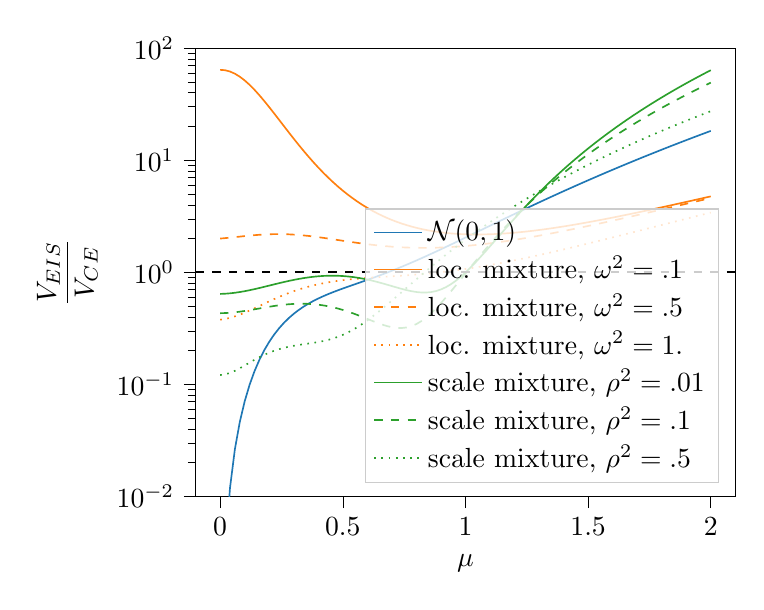
\begin{tikzpicture}

\definecolor{darkgray176}{RGB}{176,176,176}
\definecolor{darkorange25512714}{RGB}{255,127,14}
\definecolor{forestgreen4416044}{RGB}{44,160,44}
\definecolor{lightgray204}{RGB}{204,204,204}
\definecolor{steelblue31119180}{RGB}{31,119,180}

\begin{axis}[
legend cell align={left},
legend style={
  fill opacity=0.8,
  draw opacity=1,
  text opacity=1,
  at={(0.97,0.03)},
  anchor=south east,
  draw=lightgray204
},
log basis y={10},
tick align=outside,
tick pos=left,
x grid style={darkgray176},
xlabel={\(\displaystyle \mu\)},
xmin=-0.1, xmax=2.1,
xtick style={color=black},
y grid style={darkgray176},
ylabel={\(\displaystyle \frac{V_{\text{EIS}}}{V_{\text{CE}}}\)},
ymin=0.01, ymax=100,
ymode=log,
ytick style={color=black}
]
\addplot [semithick, steelblue31119180]
table {%
0 0
0.0199999995529652 0.00299281300976872
0.0399999991059303 0.0118856830522418
0.0599999986588955 0.0264268033206463
0.0799999982118607 0.0462124161422253
0.0999999940395355 0.0707092434167862
0.119999997317791 0.0992832705378532
0.140000000596046 0.131232619285583
0.159999996423721 0.165821358561516
0.179999992251396 0.202313810586929
0.199999988079071 0.240004301071167
0.219999998807907 0.278243839740753
0.239999994635582 0.31645929813385
0.259999990463257 0.35416966676712
0.280000001192093 0.390992254018784
0.299999982118607 0.426646500825882
0.319999992847443 0.46095085144043
0.340000003576279 0.493818193674088
0.359999984502792 0.525244355201721
0.379999995231628 0.555299520492554
0.399999976158142 0.584115505218506
0.419999986886978 0.611874043941498
0.439999997615814 0.638795375823975
0.459999978542328 0.665127098560333
0.479999989271164 0.691136360168457
0.5 0.717100322246552
0.519999980926514 0.743300557136536
0.539999961853027 0.770016372203827
0.560000002384186 0.797523856163025
0.579999983310699 0.826088905334473
0.599999964237213 0.855968296527863
0.620000004768372 0.887409210205078
0.639999985694885 0.920644283294678
0.659999966621399 0.955896973609924
0.680000007152557 0.993378877639771
0.699999988079071 1.03329133987427
0.719999969005585 1.0758261680603
0.740000009536743 1.1211678981781
0.759999990463257 1.16949236392975
0.779999971389771 1.22096979618073
0.799999952316284 1.27576732635498
0.819999992847443 1.33404433727264
0.839999973773956 1.39596247673035
0.85999995470047 1.46167659759521
0.879999995231628 1.53134441375732
0.899999976158142 1.6051197052002
0.919999957084656 1.68316090106964
0.939999997615814 1.76562368869781
0.959999978542328 1.85266888141632
0.979999959468842 1.94445705413818
1 2.04115223884583
1.01999998092651 2.14292287826538
1.03999996185303 2.24993705749512
1.05999994277954 2.36237406730652
1.07999992370605 2.48040914535522
1.10000002384186 2.60422539710999
1.12000000476837 2.73401188850403
1.13999998569489 2.86996269226074
1.1599999666214 3.01227259635925
1.17999994754791 3.16114592552185
1.19999992847443 3.31679320335388
1.22000002861023 3.47942614555359
1.24000000953674 3.64926242828369
1.25999999046326 3.82653069496155
1.27999997138977 4.01145696640015
1.29999995231628 4.20428419113159
1.3199999332428 4.40524911880493
1.33999991416931 4.61460781097412
1.36000001430511 4.83261156082153
1.37999999523163 5.0595235824585
1.39999997615814 5.29561042785645
1.41999995708466 5.54114484786987
1.43999993801117 5.79641771316528
1.45999991893768 6.06170701980591
1.48000001907349 6.33731842041016
1.5 6.62354278564453
1.51999998092651 6.92069721221924
1.53999996185303 7.2290940284729
1.55999994277954 7.54905796051025
1.57999992370605 7.88092231750488
1.59999990463257 8.22502326965332
1.62000000476837 8.58170700073242
1.63999998569489 8.95132637023926
1.6599999666214 9.33424663543701
1.67999994754791 9.73083209991455
1.69999992847443 10.1414632797241
1.71999990940094 10.5665254592896
1.74000000953674 11.0064125061035
1.75999999046326 11.461519241333
1.77999997138977 11.9322690963745
1.79999995231628 12.4190721511841
1.8199999332428 12.9223594665527
1.83999991416931 13.4425640106201
1.86000001430511 13.9801349639893
1.87999999523163 14.5355319976807
1.89999997615814 15.109203338623
1.91999995708466 15.7016410827637
1.93999993801117 16.3133029937744
1.95999991893768 16.944709777832
1.9799998998642 17.596342086792
2 18.268726348877
};
\addlegendentry{$\mathcal N (0,1)$}
\addplot [semithick, darkorange25512714]
table {%
0 64.064826965332
0.0199999995529652 63.5564765930176
0.0399999991059303 61.8869285583496
0.0599999986588955 59.1853523254395
0.0799999982118607 55.6484870910645
0.0999999940395355 51.5253372192383
0.119999997317791 47.0613288879395
0.140000000596046 42.4868774414062
0.159999996423721 37.9917297363281
0.179999992251396 33.7195587158203
0.199999988079071 29.7637310028076
0.219999998807907 26.1763401031494
0.239999994635582 22.974588394165
0.259999990463257 20.1525440216064
0.280000001192093 17.6916198730469
0.299999982118607 15.5568208694458
0.319999992847443 13.7170066833496
0.340000003576279 12.134391784668
0.359999984502792 10.7763261795044
0.379999995231628 9.61130809783936
0.399999976158142 8.61177158355713
0.419999986886978 7.75361347198486
0.439999997615814 7.01570272445679
0.459999978542328 6.37912464141846
0.479999989271164 5.82968711853027
0.5 5.35449600219727
0.519999980926514 4.94199657440186
0.539999961853027 4.58309888839722
0.560000002384186 4.27036666870117
0.579999983310699 3.99697470664978
0.599999964237213 3.75787019729614
0.620000004768372 3.54797673225403
0.639999985694885 3.36348152160645
0.659999966621399 3.20135378837585
0.680000007152557 3.05821967124939
0.699999988079071 2.9323935508728
0.719999969005585 2.82139372825623
0.740000009536743 2.72358298301697
0.759999990463257 2.63746047019958
0.779999971389771 2.56183743476868
0.799999952316284 2.49527978897095
0.819999992847443 2.43728399276733
0.839999973773956 2.38683366775513
0.85999995470047 2.34301543235779
0.879999995231628 2.30551099777222
0.899999976158142 2.27377128601074
0.919999957084656 2.24694991111755
0.939999997615814 2.22512435913086
0.959999978542328 2.20764780044556
0.979999959468842 2.19421529769897
1 2.18456244468689
1.01999998092651 2.17864918708801
1.03999996185303 2.17585444450378
1.05999994277954 2.17647910118103
1.07999992370605 2.18004703521729
1.10000002384186 2.18641591072083
1.12000000476837 2.19540619850159
1.13999998569489 2.20709609985352
1.1599999666214 2.22135066986084
1.17999994754791 2.23808813095093
1.19999992847443 2.25703525543213
1.22000002861023 2.27835249900818
1.24000000953674 2.30202317237854
1.25999999046326 2.32757210731506
1.27999997138977 2.35555171966553
1.29999995231628 2.38543725013733
1.3199999332428 2.41768479347229
1.33999991416931 2.45174646377563
1.36000001430511 2.48791718482971
1.37999999523163 2.52616000175476
1.39999997615814 2.56625628471375
1.41999995708466 2.60849761962891
1.43999993801117 2.6527304649353
1.45999991893768 2.69915628433228
1.48000001907349 2.74737453460693
1.5 2.79764103889465
1.51999998092651 2.84996914863586
1.53999996185303 2.90410327911377
1.55999994277954 2.96054601669312
1.57999992370605 3.01908349990845
1.59999990463257 3.07936835289001
1.62000000476837 3.14185380935669
1.63999998569489 3.20663237571716
1.6599999666214 3.27349972724915
1.67999994754791 3.3422269821167
1.69999992847443 3.41333818435669
1.71999990940094 3.4867217540741
1.74000000953674 3.56236910820007
1.75999999046326 3.64020657539368
1.77999997138977 3.72048020362854
1.79999995231628 3.80220317840576
1.8199999332428 3.88699460029602
1.83999991416931 3.97393751144409
1.86000001430511 4.06380605697632
1.87999999523163 4.15581321716309
1.89999997615814 4.24964284896851
1.91999995708466 4.34675121307373
1.93999993801117 4.44652795791626
1.95999991893768 4.54832172393799
1.9799998998642 4.65282487869263
2 4.76013040542603
};
\addlegendentry{loc. mixture, $\omega^2 = .1$}
\addplot [semithick, darkorange25512714, dashed]
table {%
0 2.00069522857666
0.0199999995529652 2.01893544197083
0.0399999991059303 2.03916788101196
0.0599999986588955 2.06059384346008
0.0799999982118607 2.08271288871765
0.0999999940395355 2.104811668396
0.119999997317791 2.12611389160156
0.140000000596046 2.14572048187256
0.159999996423721 2.16260409355164
0.179999992251396 2.17632699012756
0.199999988079071 2.18627309799194
0.219999998807907 2.19204640388489
0.239999994635582 2.19331979751587
0.259999990463257 2.19000911712646
0.280000001192093 2.18212580680847
0.299999982118607 2.17002725601196
0.319999992847443 2.15391874313354
0.340000003576279 2.13435339927673
0.359999984502792 2.11190557479858
0.379999995231628 2.08684968948364
0.399999976158142 2.05977344512939
0.419999986886978 2.03130769729614
0.439999997615814 2.00194215774536
0.459999978542328 1.9720733165741
0.479999989271164 1.94231700897217
0.5 1.91301023960114
0.519999980926514 1.88432276248932
0.539999961853027 1.8565262556076
0.560000002384186 1.83018958568573
0.579999983310699 1.80532610416412
0.599999964237213 1.78206503391266
0.620000004768372 1.76049137115479
0.639999985694885 1.74076700210571
0.659999966621399 1.72314190864563
0.680000007152557 1.70743608474731
0.699999988079071 1.69368612766266
0.719999969005585 1.68187594413757
0.740000009536743 1.67216825485229
0.759999990463257 1.66455709934235
0.779999971389771 1.65888130664825
0.799999952316284 1.65507483482361
0.819999992847443 1.65333020687103
0.839999973773956 1.65329813957214
0.85999995470047 1.65522015094757
0.879999995231628 1.65903806686401
0.899999976158142 1.66466951370239
0.919999957084656 1.67203342914581
0.939999997615814 1.68107354640961
0.959999978542328 1.69188868999481
0.979999959468842 1.70455515384674
1 1.71860444545746
1.01999998092651 1.7344559431076
1.03999996185303 1.75194537639618
1.05999994277954 1.77100145816803
1.07999992370605 1.79161584377289
1.10000002384186 1.81383836269379
1.12000000476837 1.83763337135315
1.13999998569489 1.86311709880829
1.1599999666214 1.89009070396423
1.17999994754791 1.91854846477509
1.19999992847443 1.94862055778503
1.22000002861023 1.98023450374603
1.24000000953674 2.01352310180664
1.25999999046326 2.04807043075562
1.27999997138977 2.08449840545654
1.29999995231628 2.1223464012146
1.3199999332428 2.16183733940125
1.33999991416931 2.20312261581421
1.36000001430511 2.24573850631714
1.37999999523163 2.28995490074158
1.39999997615814 2.33602571487427
1.41999995708466 2.38379645347595
1.43999993801117 2.43310904502869
1.45999991893768 2.48427653312683
1.48000001907349 2.53690695762634
1.5 2.59157562255859
1.51999998092651 2.64779663085938
1.53999996185303 2.70588898658752
1.55999994277954 2.76579260826111
1.57999992370605 2.82734560966492
1.59999990463257 2.89090061187744
1.62000000476837 2.95633316040039
1.63999998569489 3.02378416061401
1.6599999666214 3.09329605102539
1.67999994754791 3.16447877883911
1.69999992847443 3.23782467842102
1.71999990940094 3.31328535079956
1.74000000953674 3.39060592651367
1.75999999046326 3.47004723548889
1.77999997138977 3.55179619789124
1.79999995231628 3.6357638835907
1.8199999332428 3.72163438796997
1.83999991416931 3.80955243110657
1.86000001430511 3.8999650478363
1.87999999523163 3.99296545982361
1.89999997615814 4.08828449249268
1.91999995708466 4.18591403961182
1.93999993801117 4.28575134277344
1.95999991893768 4.38834714889526
1.9799998998642 4.49317741394043
2 4.60064125061035
};
\addlegendentry{loc. mixture, $\omega^2 = .5$}
\addplot [semithick, darkorange25512714, dotted]
table {%
0 0.3780198097229
0.0199999995529652 0.383591026067734
0.0399999991059303 0.392346382141113
0.0599999986588955 0.40420338511467
0.0799999982118607 0.418912380933762
0.0999999940395355 0.436240971088409
0.119999997317791 0.455965578556061
0.140000000596046 0.477641761302948
0.159999996423721 0.501008272171021
0.179999992251396 0.525627076625824
0.199999988079071 0.551053047180176
0.219999998807907 0.576954126358032
0.239999994635582 0.603023767471313
0.259999990463257 0.628755748271942
0.280000001192093 0.654045879840851
0.299999982118607 0.678528308868408
0.319999992847443 0.701861083507538
0.340000003576279 0.724102556705475
0.359999984502792 0.744918167591095
0.379999995231628 0.764307200908661
0.399999976158142 0.782261312007904
0.419999986886978 0.798586308956146
0.439999997615814 0.813658356666565
0.459999978542328 0.827271640300751
0.479999989271164 0.839538156986237
0.5 0.850645899772644
0.519999980926514 0.860495567321777
0.539999961853027 0.86939525604248
0.560000002384186 0.877569258213043
0.579999983310699 0.884868383407593
0.599999964237213 0.891722738742828
0.620000004768372 0.898136675357819
0.639999985694885 0.904202580451965
0.659999966621399 0.91007274389267
0.680000007152557 0.915912866592407
0.699999988079071 0.921836674213409
0.719999969005585 0.927826166152954
0.740000009536743 0.934146344661713
0.759999990463257 0.940782427787781
0.779999971389771 0.947908997535706
0.799999952316284 0.955457746982574
0.819999992847443 0.963574945926666
0.839999973773956 0.972351908683777
0.85999995470047 0.981722056865692
0.879999995231628 0.991853892803192
0.899999976158142 1.00293302536011
0.919999957084656 1.01468622684479
0.939999997615814 1.02721726894379
0.959999978542328 1.04079449176788
0.979999959468842 1.0552282333374
1 1.07043588161469
1.01999998092651 1.0867714881897
1.03999996185303 1.10398888587952
1.05999994277954 1.12225472927094
1.07999992370605 1.14145112037659
1.10000002384186 1.16178297996521
1.12000000476837 1.18317472934723
1.13999998569489 1.20562529563904
1.1599999666214 1.22905290126801
1.17999994754791 1.25363302230835
1.19999992847443 1.2791930437088
1.22000002861023 1.30598258972168
1.24000000953674 1.33391487598419
1.25999999046326 1.36300957202911
1.27999997138977 1.39324820041656
1.29999995231628 1.42462730407715
1.3199999332428 1.45722818374634
1.33999991416931 1.49101066589355
1.36000001430511 1.52612435817719
1.37999999523163 1.56234955787659
1.39999997615814 1.59977674484253
1.41999995708466 1.6385657787323
1.43999993801117 1.67867243289948
1.45999991893768 1.72011995315552
1.48000001907349 1.76275265216827
1.5 1.80691862106323
1.51999998092651 1.85232508182526
1.53999996185303 1.89904987812042
1.55999994277954 1.94736993312836
1.57999992370605 1.99692583084106
1.59999990463257 2.04835987091064
1.62000000476837 2.10073494911194
1.63999998569489 2.15497756004333
1.6599999666214 2.21064519882202
1.67999994754791 2.26769685745239
1.69999992847443 2.32651782035828
1.71999990940094 2.38669061660767
1.74000000953674 2.44890451431274
1.75999999046326 2.51238441467285
1.77999997138977 2.57789444923401
1.79999995231628 2.64457964897156
1.8199999332428 2.71349453926086
1.83999991416931 2.78379058837891
1.86000001430511 2.85617685317993
1.87999999523163 2.93024301528931
1.89999997615814 3.006023645401
1.91999995708466 3.08377742767334
1.93999993801117 3.16390132904053
1.95999991893768 3.24548172950745
1.9799998998642 3.32905507087708
2 3.41476202011108
};
\addlegendentry{loc. mixture, $\omega^2 = 1.$}
\addplot [semithick, forestgreen4416044]
table {%
0 0.641549170017242
0.0199999995529652 0.64431893825531
0.0399999991059303 0.649595081806183
0.0599999986588955 0.657183468341827
0.0799999982118607 0.667025923728943
0.0999999940395355 0.678922235965729
0.119999997317791 0.69266951084137
0.140000000596046 0.708047330379486
0.159999996423721 0.72487860918045
0.179999992251396 0.742746412754059
0.199999988079071 0.761478185653687
0.219999998807907 0.780706763267517
0.239999994635582 0.800100564956665
0.259999990463257 0.819344460964203
0.280000001192093 0.838056325912476
0.299999982118607 0.855963170528412
0.319999992847443 0.872696399688721
0.340000003576279 0.887921333312988
0.359999984502792 0.90135669708252
0.379999995231628 0.912797629833221
0.399999976158142 0.921839535236359
0.419999986886978 0.928400635719299
0.439999997615814 0.932246029376984
0.459999978542328 0.933306455612183
0.479999989271164 0.931405127048492
0.5 0.926657855510712
0.519999980926514 0.918972373008728
0.539999961853027 0.908493518829346
0.560000002384186 0.895359694957733
0.579999983310699 0.879699409008026
0.599999964237213 0.861952662467957
0.620000004768372 0.842281997203827
0.639999985694885 0.821190237998962
0.659999966621399 0.799105584621429
0.680000007152557 0.776510059833527
0.699999988079071 0.753969848155975
0.719999969005585 0.732140600681305
0.740000009536743 0.711811482906342
0.759999990463257 0.693664908409119
0.779999971389771 0.678595244884491
0.799999952316284 0.667292058467865
0.819999992847443 0.660893797874451
0.839999973773956 0.660263419151306
0.85999995470047 0.666379451751709
0.879999995231628 0.680451810359955
0.899999976158142 0.703445613384247
0.919999957084656 0.73673552274704
0.939999997615814 0.781327962875366
0.959999978542328 0.838589429855347
0.979999959468842 0.909819364547729
1 0.996338188648224
1.01999998092651 1.09936475753784
1.03999996185303 1.22058129310608
1.05999994277954 1.36126148700714
1.07999992370605 1.52287292480469
1.10000002384186 1.707066655159
1.12000000476837 1.91545069217682
1.13999998569489 2.14914798736572
1.1599999666214 2.41020560264587
1.17999994754791 2.70034289360046
1.19999992847443 3.02098512649536
1.22000002861023 3.37364840507507
1.24000000953674 3.760498046875
1.25999999046326 4.18283939361572
1.27999997138977 4.64322566986084
1.29999995231628 5.14264059066772
1.3199999332428 5.68347024917603
1.33999991416931 6.26725339889526
1.36000001430511 6.89635229110718
1.37999999523163 7.57224369049072
1.39999997615814 8.29694747924805
1.41999995708466 9.07260704040527
1.43999993801117 9.90093803405762
1.45999991893768 10.7841854095459
1.48000001907349 11.725682258606
1.5 12.7248392105103
1.51999998092651 13.7860450744629
1.53999996185303 14.9098329544067
1.55999994277954 16.1001052856445
1.57999992370605 17.3562240600586
1.59999990463257 18.6850242614746
1.62000000476837 20.0837936401367
1.63999998569489 21.5580883026123
1.6599999666214 23.1086921691895
1.67999994754791 24.7392253875732
1.69999992847443 26.4509201049805
1.71999990940094 28.2454490661621
1.74000000953674 30.1250629425049
1.75999999046326 32.097225189209
1.77999997138977 34.160285949707
1.79999995231628 36.3134269714355
1.8199999332428 38.5633316040039
1.83999991416931 40.9151802062988
1.86000001430511 43.3655815124512
1.87999999523163 45.9222755432129
1.89999997615814 48.5809288024902
1.91999995708466 51.3525352478027
1.93999993801117 54.2337951660156
1.95999991893768 57.2334403991699
1.9799998998642 60.3448219299316
2 63.5767211914062
};
\addlegendentry{scale mixture, $\rho^2 = .01$}
\addplot [semithick, forestgreen4416044, dashed]
table {%
0 0.431960076093674
0.0199999995529652 0.433056831359863
0.0399999991059303 0.435767710208893
0.0599999986588955 0.439941495656967
0.0799999982118607 0.44542595744133
0.0999999940395355 0.452016234397888
0.119999997317791 0.459490418434143
0.140000000596046 0.467592298984528
0.159999996423721 0.476054310798645
0.179999992251396 0.484580397605896
0.199999988079071 0.492943942546844
0.219999998807907 0.500804126262665
0.239999994635582 0.507913053035736
0.259999990463257 0.514079451560974
0.280000001192093 0.519017457962036
0.299999982118607 0.522522687911987
0.319999992847443 0.524489223957062
0.340000003576279 0.524686455726624
0.359999984502792 0.523108839988708
0.379999995231628 0.519682228565216
0.399999976158142 0.514378011226654
0.419999986886978 0.507175981998444
0.439999997615814 0.49819153547287
0.459999978542328 0.487561643123627
0.479999989271164 0.475366055965424
0.5 0.46187162399292
0.519999980926514 0.447269201278687
0.539999961853027 0.431858837604523
0.560000002384186 0.415910810232162
0.579999983310699 0.399799138307571
0.599999964237213 0.383918792009354
0.620000004768372 0.368691802024841
0.639999985694885 0.354550391435623
0.659999966621399 0.342012405395508
0.680000007152557 0.331595987081528
0.699999988079071 0.323786348104477
0.719999969005585 0.319222748279572
0.740000009536743 0.318477779626846
0.759999990463257 0.322177350521088
0.779999971389771 0.331035614013672
0.799999952316284 0.345633983612061
0.819999992847443 0.366783529520035
0.839999973773956 0.395111232995987
0.85999995470047 0.431392908096313
0.879999995231628 0.476510286331177
0.899999976158142 0.531041920185089
0.919999957084656 0.595907509326935
0.939999997615814 0.672023236751556
0.959999978542328 0.760107338428497
0.979999959468842 0.86113303899765
1 0.975934863090515
1.01999998092651 1.10541725158691
1.03999996185303 1.25050210952759
1.05999994277954 1.41215014457703
1.07999992370605 1.59141767024994
1.10000002384186 1.78918254375458
1.12000000476837 2.00641775131226
1.13999998569489 2.24426865577698
1.1599999666214 2.50348520278931
1.17999994754791 2.78554940223694
1.19999992847443 3.09129929542542
1.22000002861023 3.42165207862854
1.24000000953674 3.77817273139954
1.25999999046326 4.16154623031616
1.27999997138977 4.57310009002686
1.29999995231628 5.01390361785889
1.3199999332428 5.48514127731323
1.33999991416931 5.98850870132446
1.36000001430511 6.52421522140503
1.37999999523163 7.09415864944458
1.39999997615814 7.70020008087158
1.41999995708466 8.34212303161621
1.43999993801117 9.02214241027832
1.45999991893768 9.74127292633057
1.48000001907349 10.5009927749634
1.5 11.3029270172119
1.51999998092651 12.1473913192749
1.53999996185303 13.0371160507202
1.55999994277954 13.9729070663452
1.57999992370605 14.9544773101807
1.59999990463257 15.98681640625
1.62000000476837 17.0685005187988
1.63999998569489 18.2016181945801
1.6599999666214 19.3886241912842
1.67999994754791 20.6310119628906
1.69999992847443 21.9286193847656
1.71999990940094 23.2820262908936
1.74000000953674 24.6971664428711
1.75999999046326 26.1724376678467
1.77999997138977 27.7106800079346
1.79999995231628 29.3114318847656
1.8199999332428 30.9794292449951
1.83999991416931 32.7136878967285
1.86000001430511 34.5172996520996
1.87999999523163 36.3912544250488
1.89999997615814 38.3366241455078
1.91999995708466 40.3568916320801
1.93999993801117 42.4531707763672
1.95999991893768 44.6266937255859
1.9799998998642 46.8779067993164
2 49.2078704833984
};
\addlegendentry{scale mixture, $\rho^2 = .1$}
\addplot [semithick, forestgreen4416044, dotted]
table {%
0 0.121202975511551
0.0199999995529652 0.122827485203743
0.0399999991059303 0.126581713557243
0.0599999986588955 0.132203876972198
0.0799999982118607 0.139320194721222
0.0999999940395355 0.147537857294083
0.119999997317791 0.156492650508881
0.140000000596046 0.165712624788284
0.159999996423721 0.174919486045837
0.179999992251396 0.18379034101963
0.199999988079071 0.192084923386574
0.219999998807907 0.199579149484634
0.239999994635582 0.206233218312263
0.259999990463257 0.212016507983208
0.280000001192093 0.216982245445251
0.299999982118607 0.221204429864883
0.319999992847443 0.22487773001194
0.340000003576279 0.228213861584663
0.359999984502792 0.231481283903122
0.379999995231628 0.234899446368217
0.399999976158142 0.2388616502285
0.419999986886978 0.243608683347702
0.439999997615814 0.249434918165207
0.459999978542328 0.256711393594742
0.479999989271164 0.265735507011414
0.5 0.276754647493362
0.519999980926514 0.290141433477402
0.539999961853027 0.306143820285797
0.560000002384186 0.324998885393143
0.579999983310699 0.347046375274658
0.599999964237213 0.37250155210495
0.620000004768372 0.401553124189377
0.639999985694885 0.434563517570496
0.659999966621399 0.47167244553566
0.680000007152557 0.513170957565308
0.699999988079071 0.559247255325317
0.719999969005585 0.610128819942474
0.740000009536743 0.665990650653839
0.759999990463257 0.727211236953735
0.779999971389771 0.793849647045135
0.799999952316284 0.86616313457489
0.819999992847443 0.944479048252106
0.839999973773956 1.02896189689636
0.85999995470047 1.11980056762695
0.879999995231628 1.21729755401611
0.899999976158142 1.32162249088287
0.919999957084656 1.43319511413574
0.939999997615814 1.55205357074738
0.959999978542328 1.67853903770447
0.979999959468842 1.81309962272644
1 1.95563971996307
1.01999998092651 2.10671281814575
1.03999996185303 2.26648712158203
1.05999994277954 2.43537926673889
1.07999992370605 2.61347460746765
1.10000002384186 2.80138826370239
1.12000000476837 2.99910187721252
1.13999998569489 3.20709419250488
1.1599999666214 3.42573642730713
1.17999994754791 3.65518379211426
1.19999992847443 3.89602303504944
1.22000002861023 4.14815378189087
1.24000000953674 4.41241598129272
1.25999999046326 4.6890082359314
1.27999997138977 4.97817993164062
1.29999995231628 5.28051900863647
1.3199999332428 5.59601020812988
1.33999991416931 5.92562246322632
1.36000001430511 6.26900959014893
1.37999999523163 6.62697219848633
1.39999997615814 7.00068664550781
1.41999995708466 7.3888988494873
1.43999993801117 7.79298543930054
1.45999991893768 8.21372413635254
1.48000001907349 8.65087413787842
1.5 9.10478591918945
1.51999998092651 9.57632350921631
1.53999996185303 10.0661001205444
1.55999994277954 10.5744380950928
1.57999992370605 11.1009254455566
1.59999990463257 11.6468868255615
1.62000000476837 12.2130117416382
1.63999998569489 12.7992753982544
1.6599999666214 13.4059896469116
1.67999994754791 14.0341806411743
1.69999992847443 14.6842613220215
1.71999990940094 15.3561315536499
1.74000000953674 16.0509414672852
1.75999999046326 16.7691287994385
1.77999997138977 17.5110683441162
1.79999995231628 18.2770843505859
1.8199999332428 19.0684509277344
1.83999991416931 19.8845062255859
1.86000001430511 20.7268753051758
1.87999999523163 21.5960102081299
1.89999997615814 22.4912719726562
1.91999995708466 23.4140129089355
1.93999993801117 24.3672466278076
1.95999991893768 25.3471813201904
1.9799998998642 26.3551006317139
2 27.3943290710449
};
\addlegendentry{scale mixture, $\rho^2 = .5$}
\addplot [semithick, black, dashed, forget plot]
table {%
-0.1 1
2.1 1
};
\end{axis}

\end{tikzpicture}
%
            }
        \end{subfigure}
        \label{fig:normal_are}
        \caption{Asymptotic relative efficiency $\frac{V_{\eis}}{V_{\ce}}$ for the normal distribution from \Cref{ex:univ-gaussian-s2-fixed} (left hand side) and \Cref{ex:univ-gaussian-mu-fixed} (right hand side). Here $\P = \mathcal N(0, 1)$ is the standard normal distribution and $\G = \mathcal N(\mu, \sigma^{2})$, where either $\sigma^{2}$ is fixed (left) and $\mu$ determined by the \gls{cem} / \gls{eis}, or the other way around (right). Notice the log scale of the $y$-axis. As $\mu$ or $\sigma^{2}$ get close to their true values, \gls{eis} outperforms the \gls{cem} in terms of asymptotic variance, see {\color{red} todo:  reference to example where EIS is exact.}. As}
    \end{figure}
    

    %\begin{table}
    %    \centering
    %    \begin{tabular}{ccc}
    %        \toprule
    %        & $\sigma^{2}$ fixed, $\tau^{2} \to \infty$ & $\tau^{2}$ fixed, $\sigma^{2} \to \infty$\\
    %        \midrule
    %        $V_{\ce} / V_{\eis}$ & $\frac{2}{5} \sigma^{2}$ & 0 \\
    %        \bottomrule
    %    \end{tabular}
    %    \caption{Relative asymptotic efficiencies of the \gls{cem} and \gls{eis} for \Cref{ex:univ-gaussian-s2-fixed} and \Cref{ex:univ-gaussian-mu-fixed}.}
    %    \label{tab:comparison-asymptotics}
    %\end{table}
    
    \paragraph{Gaussian location mixture}
    Consider now the case where $\P = \frac{1}{2} \mathcal N(-1, \omega^{2}) + \frac{1}{2}\mathcal N(1, \omega^{2})$ is a Gaussian location mixture. The second moment is $\tau^{2} = 1 + \omega^{2} = -\frac{1}{2\pce}$. Unfortunately, there is no closed-form expression for many of the terms required for the analysis \gls{eis}. Instead, we resort to a simulation study to determine the asymptotic variances and relative efficiencies.

    \todo{numerical example: GMM}
    \todo{interpretation: if variance set too low, CE better. if variance too big EIS better}
    
\end{example}

\begin{example}[univariate Gaussian, $\mu$ fixed]
    \label{ex:univ-gaussian-mu-fixed}
    Consider the same setup as in \Cref{ex:univ-gaussian-s2-fixed}, i.e. $\P$ is symmetric around $0$ with second moment $\tau^{2}$, but let $\G_{\psi} = \mathcal N(\mu, -\frac{1}{2\psi})$ be the single parameter natural exponential family of Gaussians with fixed mean $\mu$ and variance $\sigma^{2} = -\frac{1}{2 \psi}$. 
    
    Then
    $$
    \log g_{\psi}(x) = \psi T(x) + \frac{1}{2}\log \left( - 2 \psi \right) - \frac{1}{2} \log 2\pi
    $$
    for $T(x) = (x - \mu)^{2}$. Thus $\P T = \tau^{2} + \mu^{2}$ and $\cov_{\P} T = \nu - \tau^{4} + 4\tau^{2}\mu^{2}$ where $\nu = \P \operatorname{id}^{4}$ and $\tau^{2} = \P \id^{2}$. 
    %\paragraph{\Acrlong{cem}}

    By matching moments, we obtain $\pce = -\frac{1}{2(\tau^{2} + \mu^{2})}$ and $I(\pce) = \frac{1}{2\pce^{2}} = 2(\tau^{2} + \mu^{2})^{2}$. In total 
    \begin{align}
        V_{\ce} &= \frac{1}{4 (\tau^{2} + \mu^{2})^{4}} \left( \nu - \tau^{4} + 4\tau^{2}\mu^{2} \right)
    \end{align}

    %\paragraph{\Acrlong{eis}}
    For \gls{eis},
    \begin{align*}
    \peis &= \left( \cov_{\P} T \right)^{-1} \cov_{\P} \left( T, \log p \right) \\
        &= \left( \nu - \tau^{4} + 4\tau^{2}\mu^{2} \right)^{-1} \underbrace{\int p(x)((x-\mu)^{2}-\tau^{2} - \mu^{2})(\log p(x) - \P\log p(x)) \d x}_{=\gamma}.
    \end{align*}
    
    Then 
    \begin{align*}
        V_{\eis} = \left( \nu - \tau^{4} + 4 \tau^{2}\mu^{2}\right)^{-2} \P \left( (\id - \mu)^{4} \left( \log p - \peis (\id - \mu)^{2} - \P \log p + \psi (\tau^{2} + \mu^{2}) \right)^{2} \right).
    \end{align*}

    \paragraph{Normal distribution}
    Consider now the normal distribution $\P = \mathcal N (0, \tau^{2})$ where $\nu = 3 \tau^{4}$ and $\gamma = -\tau^{2}$, so 
    \begin{align*}
        \peis &= \frac{-\tau^{2}}{2\tau^{2} \left( \tau^{2} + 2\mu^{2} \right)} = \frac{-1}{2(\tau^{2} + 2\mu^{2})}.
    \end{align*}
    Thus the \gls{eis} proposal uses variance $\sigma^{2}_{\eis} = \tau^{2} + 2\mu^{2}$, which is bigger than the variance of $\sigma^{2}_{\ce} = \tau^{2} + \mu^{2}$ optimal for the \gls{cem}.

    In this case the asymptotic variances are
    \begin{align*}
    %\label{eq:asymptotic-vars}
        V_{\ce} &= \frac{\tau^{2}(\tau^{2} + 2\mu^{2})}{2 \left( \tau^{2} + \mu^{2} \right)^{4}}\\
        \intertext{and}
        V_{\eis} &= \frac{\mu^{2} \left(2 \mu^{6} + 45 \mu^{4} \tau^{2} + 15 \tau^{6}\right)}{4 \tau^{4} \left(2 \mu^{2} + \tau^{2}\right)^{4}},
    \end{align*}
    see the accompanying source code for their calculation in sympy \todo{ref it}.
\end{example}


% rationale
In applications, e.g. the model studied in \Cref{cha:analysis_of_selected_models}, we are interested in the performance of the importance sampling proposals generated by the \gls{la}, \gls{cem} and \gls{eis} under more complex circumstances than those discussed in \Cref{ex:univ-gaussian-mu-fixed,ex:univ-gaussian-s2-fixed}. In particular, the dimension of $\psi$ is high ($\mathcal O(n \cdot m)$ or even $\mathcal O(n \cdot m^{2})$) and proposals may not come from a natural exponential family, so analysis based on \Cref{thm:ce-clt,thm:clt-eis} is not possible. Instead, we resort to simulation studies to gain insights into the circumstances when one should prefer one method over the other.
As a leading example, we will use the following vector-autoregressive state space model with negative binomial observations. A similar, though more involved, model is studied in \Cref{sec:regional_growth_factor_model} with real data.

\begin{example}[Negative Binomial $\operatorname{VAR}(1)$ \gls{ssm}]
    \label{ex:negbinom-ar1}
    % setup 
    In this example, we consider a \gls{ssm} where states $X_{t}$ follow a stationary Gaussian $\operatorname{VAR}(1)$ process, initialized in its stationary distribution $\mathcal N(0,\Sigma)$. For simplicity let the transition matrices be given by a multiple of the identity, i.e. $A_{t} = \alpha I_{m}$ for all $t$ where $\alpha \in (-1, 1)$ \todo{add I to symbols}. 
    In total, the model is given by
    \begin{align*}
    X_{0} &\sim \mathcal N(0,\Sigma) \\
    X_{t} &= \alpha X_{t - 1} + \varepsilon_{t}\\
    \varepsilon_t &\iid \mathcal N(0, (1 - \alpha^{2})\Sigma), t = 1, \dots, n
    \end{align*}
    where the $\varepsilon_{1}, \dots, n$ and $X_{0}$ are jointly independent. The observations follow a conditional negative binomial distribution 
    $$
    Y^{i}_{t} | X_{t} \sim \nbinom \left( \exp{X^{i}_{t}}, r \right), i = 1, \dots, p
    $$
    where the parametrization is the one by mean and overdispersion parameter $r > 0$ \todo{ref it} and individual observations are conditionally independent given the current state.
\end{example}

%% simulation study on MSE/Bias/Variance

Our first simulation study concerns the non-asymptotic behavior of the \gls{cem} and \gls{eis} estimators, i.e. finite sample analogs of \Cref{thm:ce-clt,thm:clt-eis}. To this end,
we let $m = 1$ in \Cref{ex:negbinom-ar1} and fix $n$ to \todo{...}. 
We then simulate once from the marginal distribution of $Y$ and perform the \gls{la} to a prespecified precision $\epsilon$ and maximum number of iterations $n_{\text{iter}}$, obtaining a proposal distribution $\G_{\la}$. Using a large number of samples $N_{\text{true}}$ from this proposal we find the optimal $\G_{\ce}$ and $\G_{\eis}$ using the same desired precision and number of iterations as for the \gls{la}. For the remainder of this section, we ignore sampling variation in these proposals and treat them as exact. 

%% posterior marginal means and variances
To determine the non-asymptotic sampling behavior we now perform the above procedure again, using only $N \ll N_{\text{true}}$ many samples for both procedures, obtaining proposals $\hat\P^{N}_{\ce}$ and $\hat \P^{N}_{\eis}$. As the full proposals are Gaussian distributions on $\R^{(n+1)\times m}$, either given as the posterior of a \gls{glssm} (\gls{la}, \gls{eis}) or by mean and Cholesky root of the precision matrix(\gls{cem}). 
This procedure is repeated $M$ times for every sample size $N$ considered, with different initial random seeds, obtaining $\hat\P^{N,i}_{\ce}$ and $\hat \P^{N,i}_{\eis}$ for $i = 1, \dots, M$.

To assess the speed of convergence of the \gls{cem} and \gls{eis} we then estimate the mean squared error of means and variances of the $(n+1) \times m$ univariate marginals as $N$, the number of samples used to obtain $\hpce$ or $\hpeis$, grows. For the true value, we take the univariate means and variances of $\G_{\ce}$ and $\G_{\eis}$ respectively. Additionally, we perform a bias-variance decomposition to see where the estimation error originates. 

More concretely, fix $N$ and denote by $\mu, \sigma^{2} \in \mathbf R^{(n + 1) \cdot m}$ the marginal means and variances of $\G_{\ce}$ ($\G_{\eis}$). 
Let $\mu_{i}, \sigma^{2}_{i}\in\mathbf R^{(n + 1) \cdot m}$ be the marginal means and variances of $\G^{N,i}_{\ce}$ ($\G^{N,i}_{\eis}$) for $i = 1,\dots, M$. 
Now 
$$
\widehat{\text{ASE}_{i}} = \frac{1}{(n +1)m} \left( \lVert \mu - \mu_{i}\rVert^{2} + \lVert \sigma^{2} - \sigma^{2}_{i}\rVert^{2} \right)
$$
is an estimate of the state-average squared error and 
$$
\widehat{\text{AMSE}} = \frac{1}{M} \sum_{i = 1}^{M} \widehat{\text{ASE}_{i}}
$$
is an estimate of the state-average mean squared error. 
The $\text{ASE}_{i}$ is of interest to the practitioner as they usually only run a single iteration of the optimal importance sampling procedure. So while a low $\text{AMSE}$ is desirable, the variance of $\text{ASE}$ should also be small in practice, as otherwise several runs of the optimal importance sampling procedure may be required to obtain a good proposal.

In \Cref{fig:mse_bias_var_decomposition} we show the $\widehat{\text{ASE}_{i}}$ for $i=1, \dots, M$ for both the \gls{cem} and \gls{eis}. As is evident from this Figure, the \gls{cem} consistently has a larger average mean squared error than \gls{eis}, for all values of $N$. Thus the \gls{cem} requires several orders of magnitude more samples to obtain the same error as \gls{eis}.
\todo{more interpretation}

For further investigation we perform a bias-variance decomposition of the A(M)SE for both the means $\mu$ and variances $\sigma^{2}$. Consider the averages means and variances over the $M$ simulations,
\begin{align*}
    \bar \mu = \frac{1}{M} \sum_{i=1}^{M} \mu_{i} && \bar \sigma^{2} = \frac{1}{M} \sum_{i=1}^{M} \sigma^{2}_{i},
\end{align*}
and the state-average squared bias and variance
\begin{align*}
    \text{aBias} &= \frac{1}{(n+1)m} \lVert \mu - \bar\mu \rVert^{2} \\
    \text{aVar} &= \frac{1}{M - 1}\frac{1}{(n+1)m} \sum_{i=1}^M \lVert \bar\mu - \mu_{i} \rVert^{2}.
\end{align*}


\begin{figure}
    \resizebox{\textwidth}{!}{%
        % Created by tikzDevice version 0.12.6 on 2024-05-22 14:37:09
% !TEX encoding = UTF-8 Unicode
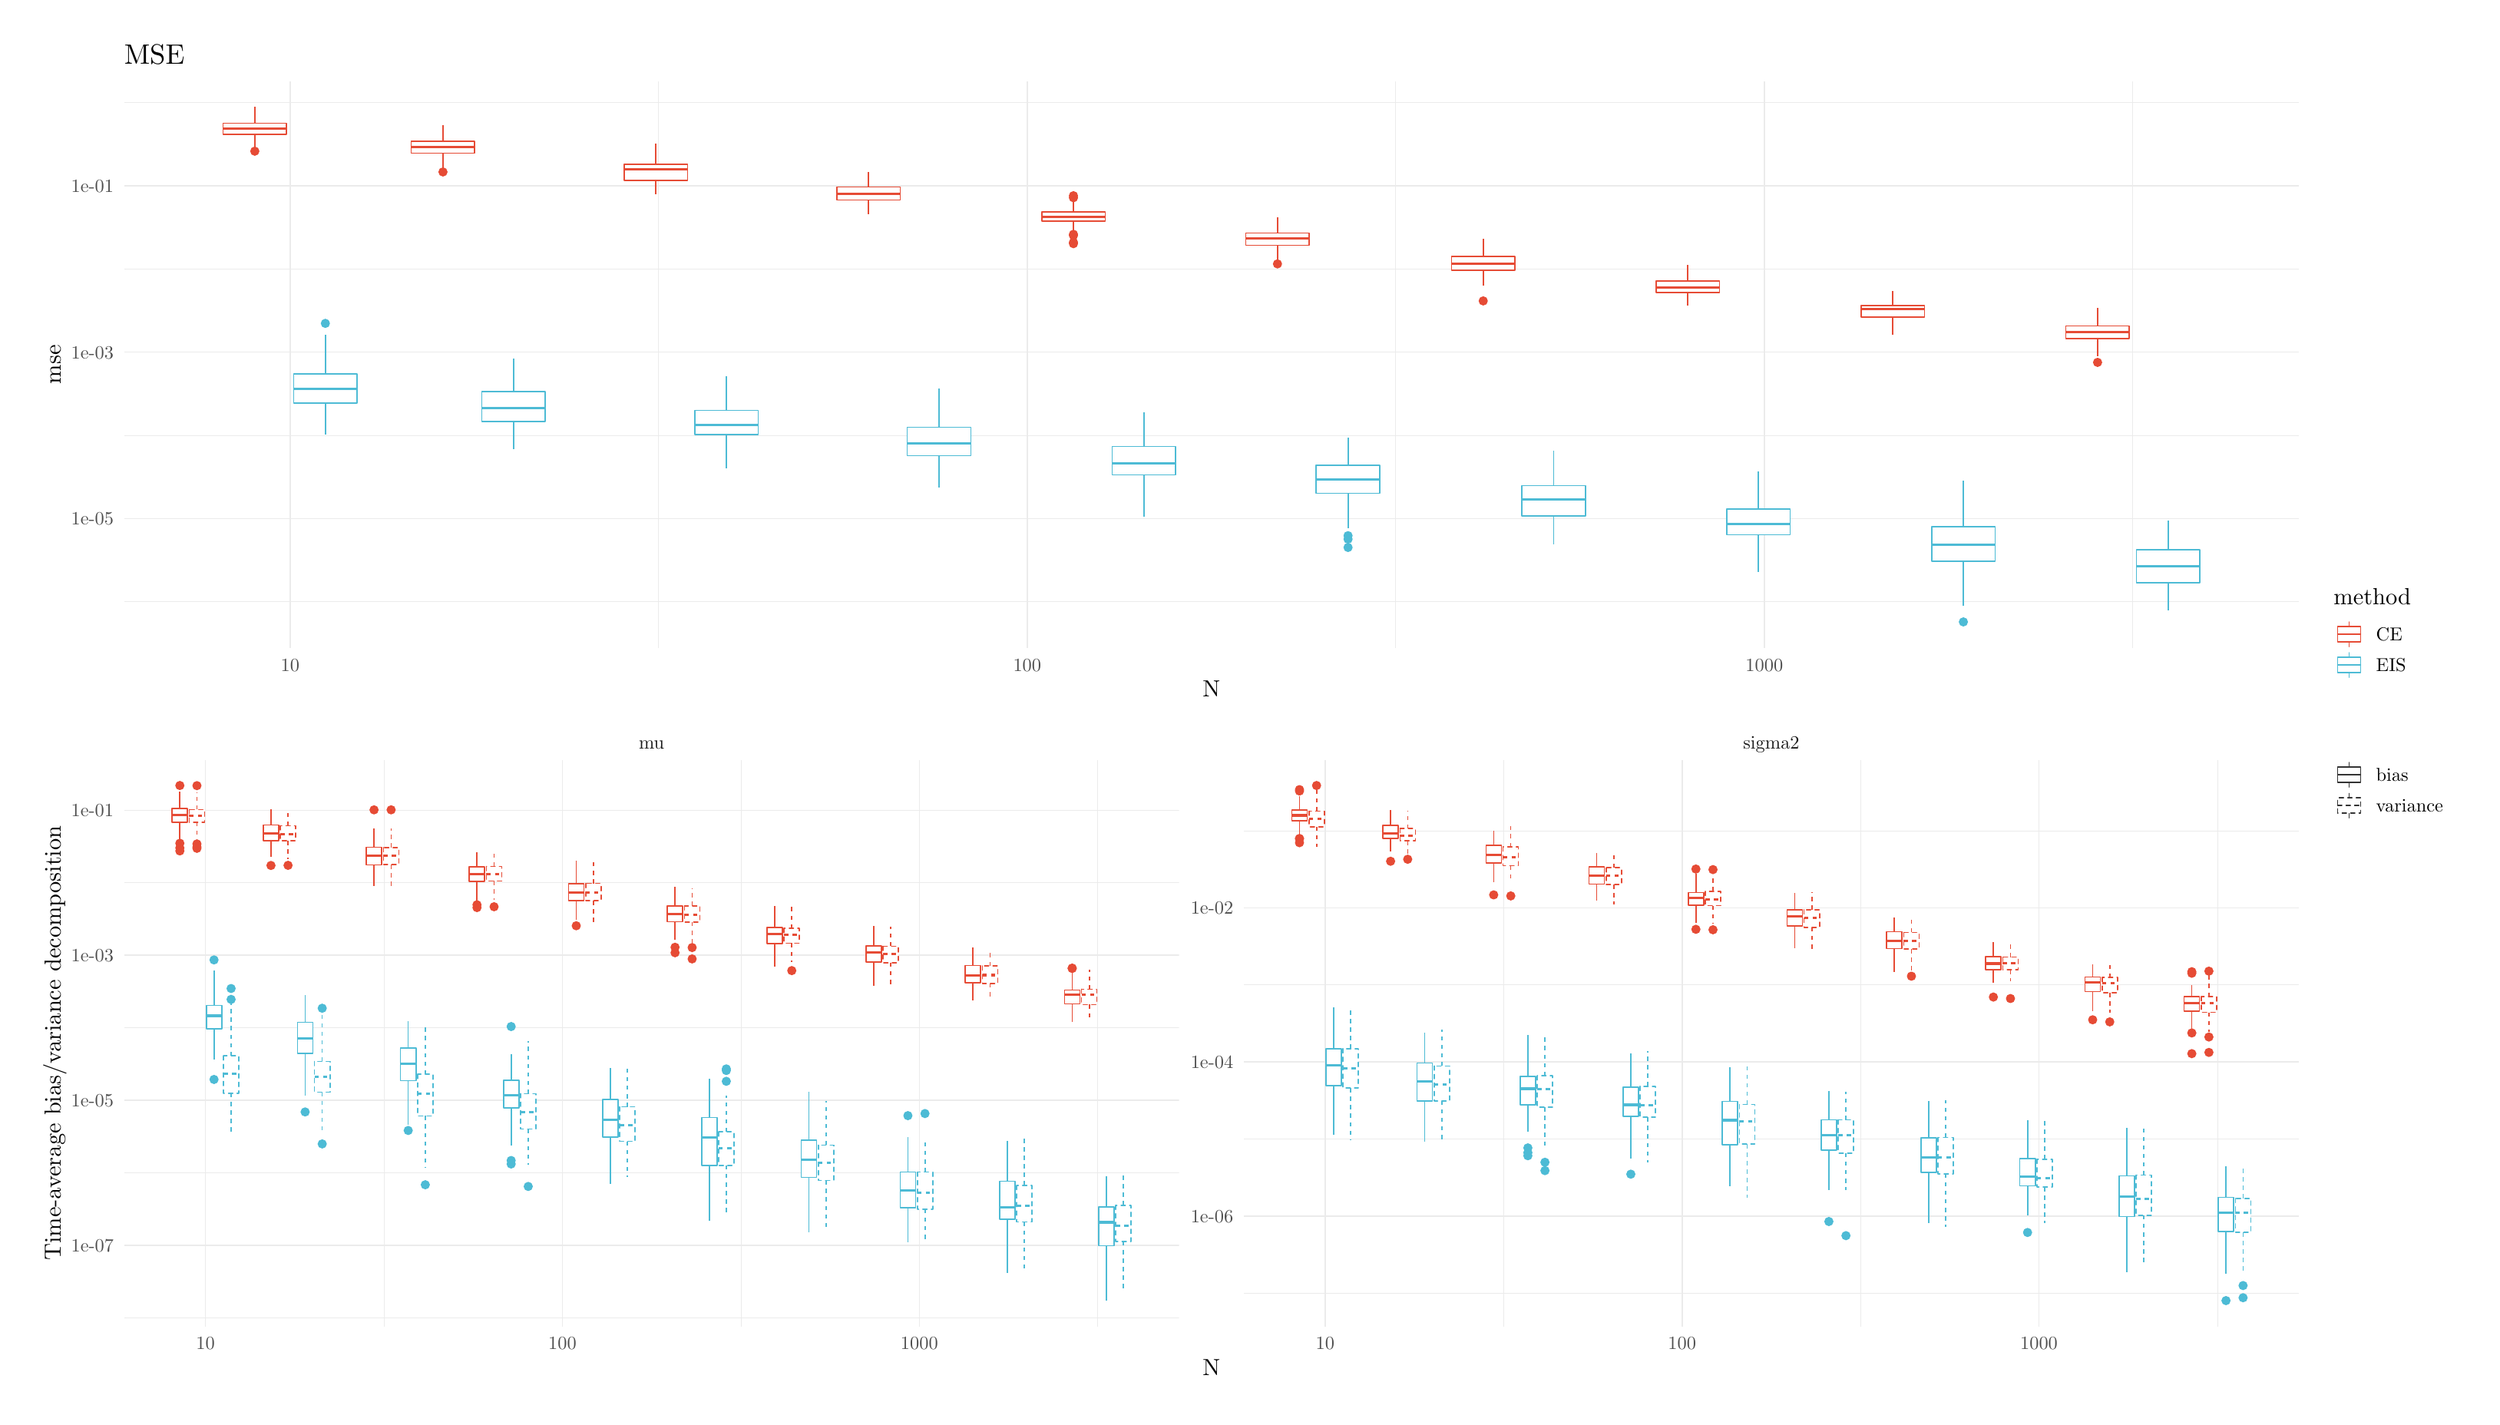
\begin{tikzpicture}[x=1pt,y=1pt]
\definecolor{fillColor}{RGB}{255,255,255}
\path[use as bounding box,fill=fillColor,fill opacity=0.00] (0,0) rectangle (1156.32,650.43);
\begin{scope}
\path[clip] ( 48.45,355.61) rectangle (1071.82,622.27);
\definecolor{drawColor}{gray}{0.92}

\path[draw=drawColor,line width= 0.3pt,line join=round] ( 48.45,377.19) --
	(1071.82,377.19);

\path[draw=drawColor,line width= 0.3pt,line join=round] ( 48.45,455.52) --
	(1071.82,455.52);

\path[draw=drawColor,line width= 0.3pt,line join=round] ( 48.45,533.86) --
	(1071.82,533.86);

\path[draw=drawColor,line width= 0.3pt,line join=round] ( 48.45,612.20) --
	(1071.82,612.20);

\path[draw=drawColor,line width= 0.3pt,line join=round] (299.97,355.61) --
	(299.97,622.27);

\path[draw=drawColor,line width= 0.3pt,line join=round] (646.87,355.61) --
	(646.87,622.27);

\path[draw=drawColor,line width= 0.3pt,line join=round] (993.77,355.61) --
	(993.77,622.27);

\path[draw=drawColor,line width= 0.6pt,line join=round] ( 48.45,416.35) --
	(1071.82,416.35);

\path[draw=drawColor,line width= 0.6pt,line join=round] ( 48.45,494.69) --
	(1071.82,494.69);

\path[draw=drawColor,line width= 0.6pt,line join=round] ( 48.45,573.03) --
	(1071.82,573.03);

\path[draw=drawColor,line width= 0.6pt,line join=round] (126.52,355.61) --
	(126.52,622.27);

\path[draw=drawColor,line width= 0.6pt,line join=round] (473.42,355.61) --
	(473.42,622.27);

\path[draw=drawColor,line width= 0.6pt,line join=round] (820.32,355.61) --
	(820.32,622.27);
\definecolor{drawColor}{RGB}{230,75,53}
\definecolor{fillColor}{RGB}{230,75,53}

\path[draw=drawColor,line width= 0.4pt,line join=round,line cap=round,fill=fillColor] (109.91,589.27) circle (  1.96);

\path[draw=drawColor,line width= 0.6pt,line join=round] (109.91,602.43) -- (109.91,610.15);

\path[draw=drawColor,line width= 0.6pt,line join=round] (109.91,597.18) -- (109.91,589.35);
\definecolor{fillColor}{RGB}{255,255,255}

\path[draw=drawColor,line width= 0.6pt,line join=round,line cap=round,fill=fillColor] ( 94.97,602.43) --
	( 94.97,597.18) --
	(124.86,597.18) --
	(124.86,602.43) --
	( 94.97,602.43) --
	cycle;

\path[draw=drawColor,line width= 1.1pt,line join=round] ( 94.97,599.88) -- (124.86,599.88);
\definecolor{fillColor}{RGB}{230,75,53}

\path[draw=drawColor,line width= 0.4pt,line join=round,line cap=round,fill=fillColor] (198.47,579.50) circle (  1.96);

\path[draw=drawColor,line width= 0.6pt,line join=round] (198.47,594.01) -- (198.47,601.62);

\path[draw=drawColor,line width= 0.6pt,line join=round] (198.47,588.28) -- (198.47,581.12);
\definecolor{fillColor}{RGB}{255,255,255}

\path[draw=drawColor,line width= 0.6pt,line join=round,line cap=round,fill=fillColor] (183.52,594.01) --
	(183.52,588.28) --
	(213.41,588.28) --
	(213.41,594.01) --
	(183.52,594.01) --
	cycle;

\path[draw=drawColor,line width= 1.1pt,line join=round] (183.52,591.17) -- (213.41,591.17);

\path[draw=drawColor,line width= 0.6pt,line join=round] (298.65,583.04) -- (298.65,592.79);

\path[draw=drawColor,line width= 0.6pt,line join=round] (298.65,575.51) -- (298.65,568.86);

\path[draw=drawColor,line width= 0.6pt,line join=round,line cap=round,fill=fillColor] (283.71,583.04) --
	(283.71,575.51) --
	(313.59,575.51) --
	(313.59,583.04) --
	(283.71,583.04) --
	cycle;

\path[draw=drawColor,line width= 1.1pt,line join=round] (283.71,580.63) -- (313.59,580.63);

\path[draw=drawColor,line width= 0.6pt,line join=round] (398.71,572.42) -- (398.71,579.51);

\path[draw=drawColor,line width= 0.6pt,line join=round] (398.71,566.26) -- (398.71,559.75);

\path[draw=drawColor,line width= 0.6pt,line join=round,line cap=round,fill=fillColor] (383.77,572.42) --
	(383.77,566.26) --
	(413.65,566.26) --
	(413.65,572.42) --
	(383.77,572.42) --
	cycle;

\path[draw=drawColor,line width= 1.1pt,line join=round] (383.77,569.10) -- (413.65,569.10);
\definecolor{fillColor}{RGB}{230,75,53}

\path[draw=drawColor,line width= 0.4pt,line join=round,line cap=round,fill=fillColor] (495.18,549.62) circle (  1.96);

\path[draw=drawColor,line width= 0.4pt,line join=round,line cap=round,fill=fillColor] (495.18,568.31) circle (  1.96);

\path[draw=drawColor,line width= 0.4pt,line join=round,line cap=round,fill=fillColor] (495.18,567.37) circle (  1.96);

\path[draw=drawColor,line width= 0.4pt,line join=round,line cap=round,fill=fillColor] (495.18,550.15) circle (  1.96);

\path[draw=drawColor,line width= 0.4pt,line join=round,line cap=round,fill=fillColor] (495.18,546.37) circle (  1.96);

\path[draw=drawColor,line width= 0.4pt,line join=round,line cap=round,fill=fillColor] (495.18,545.75) circle (  1.96);

\path[draw=drawColor,line width= 0.6pt,line join=round] (495.18,560.64) -- (495.18,566.67);

\path[draw=drawColor,line width= 0.6pt,line join=round] (495.18,556.47) -- (495.18,551.07);
\definecolor{fillColor}{RGB}{255,255,255}

\path[draw=drawColor,line width= 0.6pt,line join=round,line cap=round,fill=fillColor] (480.23,560.64) --
	(480.23,556.47) --
	(510.12,556.47) --
	(510.12,560.64) --
	(480.23,560.64) --
	cycle;

\path[draw=drawColor,line width= 1.1pt,line join=round] (480.23,558.41) -- (510.12,558.41);
\definecolor{fillColor}{RGB}{230,75,53}

\path[draw=drawColor,line width= 0.4pt,line join=round,line cap=round,fill=fillColor] (591.20,536.22) circle (  1.96);

\path[draw=drawColor,line width= 0.6pt,line join=round] (591.20,550.79) -- (591.20,558.01);

\path[draw=drawColor,line width= 0.6pt,line join=round] (591.20,545.03) -- (591.20,537.39);
\definecolor{fillColor}{RGB}{255,255,255}

\path[draw=drawColor,line width= 0.6pt,line join=round,line cap=round,fill=fillColor] (576.25,550.79) --
	(576.25,545.03) --
	(606.14,545.03) --
	(606.14,550.79) --
	(576.25,550.79) --
	cycle;

\path[draw=drawColor,line width= 1.1pt,line join=round] (576.25,548.11) -- (606.14,548.11);
\definecolor{fillColor}{RGB}{230,75,53}

\path[draw=drawColor,line width= 0.4pt,line join=round,line cap=round,fill=fillColor] (688.03,518.80) circle (  1.96);

\path[draw=drawColor,line width= 0.6pt,line join=round] (688.03,539.77) -- (688.03,548.16);

\path[draw=drawColor,line width= 0.6pt,line join=round] (688.03,533.22) -- (688.03,525.96);
\definecolor{fillColor}{RGB}{255,255,255}

\path[draw=drawColor,line width= 0.6pt,line join=round,line cap=round,fill=fillColor] (673.08,539.77) --
	(673.08,533.22) --
	(702.97,533.22) --
	(702.97,539.77) --
	(673.08,539.77) --
	cycle;

\path[draw=drawColor,line width= 1.1pt,line join=round] (673.08,536.41) -- (702.97,536.41);

\path[draw=drawColor,line width= 0.6pt,line join=round] (784.28,528.06) -- (784.28,535.76);

\path[draw=drawColor,line width= 0.6pt,line join=round] (784.28,522.86) -- (784.28,516.78);

\path[draw=drawColor,line width= 0.6pt,line join=round,line cap=round,fill=fillColor] (769.34,528.06) --
	(769.34,522.86) --
	(799.23,522.86) --
	(799.23,528.06) --
	(769.34,528.06) --
	cycle;

\path[draw=drawColor,line width= 1.1pt,line join=round] (769.34,525.06) -- (799.23,525.06);

\path[draw=drawColor,line width= 0.6pt,line join=round] (880.79,516.67) -- (880.79,523.61);

\path[draw=drawColor,line width= 0.6pt,line join=round] (880.79,511.12) -- (880.79,502.84);

\path[draw=drawColor,line width= 0.6pt,line join=round,line cap=round,fill=fillColor] (865.85,516.67) --
	(865.85,511.12) --
	(895.73,511.12) --
	(895.73,516.67) --
	(865.85,516.67) --
	cycle;

\path[draw=drawColor,line width= 1.1pt,line join=round] (865.85,514.82) -- (895.73,514.82);
\definecolor{fillColor}{RGB}{230,75,53}

\path[draw=drawColor,line width= 0.4pt,line join=round,line cap=round,fill=fillColor] (977.15,489.87) circle (  1.96);

\path[draw=drawColor,line width= 0.6pt,line join=round] (977.15,507.02) -- (977.15,515.40);

\path[draw=drawColor,line width= 0.6pt,line join=round] (977.15,501.00) -- (977.15,492.74);
\definecolor{fillColor}{RGB}{255,255,255}

\path[draw=drawColor,line width= 0.6pt,line join=round,line cap=round,fill=fillColor] (962.20,507.02) --
	(962.20,501.00) --
	(992.09,501.00) --
	(992.09,507.02) --
	(962.20,507.02) --
	cycle;

\path[draw=drawColor,line width= 1.1pt,line join=round] (962.20,504.08) -- (992.09,504.08);
\definecolor{drawColor}{RGB}{77,187,213}
\definecolor{fillColor}{RGB}{77,187,213}

\path[draw=drawColor,line width= 0.4pt,line join=round,line cap=round,fill=fillColor] (143.12,508.23) circle (  1.96);

\path[draw=drawColor,line width= 0.6pt,line join=round] (143.12,484.52) -- (143.12,502.75);

\path[draw=drawColor,line width= 0.6pt,line join=round] (143.12,470.70) -- (143.12,456.04);
\definecolor{fillColor}{RGB}{255,255,255}

\path[draw=drawColor,line width= 0.6pt,line join=round,line cap=round,fill=fillColor] (128.18,484.52) --
	(128.18,470.70) --
	(158.07,470.70) --
	(158.07,484.52) --
	(128.18,484.52) --
	cycle;

\path[draw=drawColor,line width= 1.1pt,line join=round] (128.18,477.34) -- (158.07,477.34);

\path[draw=drawColor,line width= 0.6pt,line join=round] (231.68,476.16) -- (231.68,491.74);

\path[draw=drawColor,line width= 0.6pt,line join=round] (231.68,461.96) -- (231.68,449.14);

\path[draw=drawColor,line width= 0.6pt,line join=round,line cap=round,fill=fillColor] (216.73,476.16) --
	(216.73,461.96) --
	(246.62,461.96) --
	(246.62,476.16) --
	(216.73,476.16) --
	cycle;

\path[draw=drawColor,line width= 1.1pt,line join=round] (216.73,468.25) -- (246.62,468.25);

\path[draw=drawColor,line width= 0.6pt,line join=round] (331.86,467.34) -- (331.86,483.32);

\path[draw=drawColor,line width= 0.6pt,line join=round] (331.86,455.96) -- (331.86,440.11);

\path[draw=drawColor,line width= 0.6pt,line join=round,line cap=round,fill=fillColor] (316.91,467.34) --
	(316.91,455.96) --
	(346.80,455.96) --
	(346.80,467.34) --
	(316.91,467.34) --
	cycle;

\path[draw=drawColor,line width= 1.1pt,line join=round] (316.91,460.56) -- (346.80,460.56);

\path[draw=drawColor,line width= 0.6pt,line join=round] (431.92,459.29) -- (431.92,477.47);

\path[draw=drawColor,line width= 0.6pt,line join=round] (431.92,446.02) -- (431.92,430.85);

\path[draw=drawColor,line width= 0.6pt,line join=round,line cap=round,fill=fillColor] (416.97,459.29) --
	(416.97,446.02) --
	(446.86,446.02) --
	(446.86,459.29) --
	(416.97,459.29) --
	cycle;

\path[draw=drawColor,line width= 1.1pt,line join=round] (416.97,451.75) -- (446.86,451.75);

\path[draw=drawColor,line width= 0.6pt,line join=round] (528.38,450.25) -- (528.38,466.27);

\path[draw=drawColor,line width= 0.6pt,line join=round] (528.38,436.97) -- (528.38,417.16);

\path[draw=drawColor,line width= 0.6pt,line join=round,line cap=round,fill=fillColor] (513.44,450.25) --
	(513.44,436.97) --
	(543.33,436.97) --
	(543.33,450.25) --
	(513.44,450.25) --
	cycle;

\path[draw=drawColor,line width= 1.1pt,line join=round] (513.44,442.28) -- (543.33,442.28);
\definecolor{fillColor}{RGB}{77,187,213}

\path[draw=drawColor,line width= 0.4pt,line join=round,line cap=round,fill=fillColor] (624.41,406.69) circle (  1.96);

\path[draw=drawColor,line width= 0.4pt,line join=round,line cap=round,fill=fillColor] (624.41,402.77) circle (  1.96);

\path[draw=drawColor,line width= 0.4pt,line join=round,line cap=round,fill=fillColor] (624.41,408.31) circle (  1.96);

\path[draw=drawColor,line width= 0.6pt,line join=round] (624.41,441.40) -- (624.41,454.31);

\path[draw=drawColor,line width= 0.6pt,line join=round] (624.41,428.26) -- (624.41,411.70);
\definecolor{fillColor}{RGB}{255,255,255}

\path[draw=drawColor,line width= 0.6pt,line join=round,line cap=round,fill=fillColor] (609.46,441.40) --
	(609.46,428.26) --
	(639.35,428.26) --
	(639.35,441.40) --
	(609.46,441.40) --
	cycle;

\path[draw=drawColor,line width= 1.1pt,line join=round] (609.46,434.60) -- (639.35,434.60);

\path[draw=drawColor,line width= 0.6pt,line join=round] (721.23,431.86) -- (721.23,448.33);

\path[draw=drawColor,line width= 0.6pt,line join=round] (721.23,417.63) -- (721.23,404.11);

\path[draw=drawColor,line width= 0.6pt,line join=round,line cap=round,fill=fillColor] (706.29,431.86) --
	(706.29,417.63) --
	(736.18,417.63) --
	(736.18,431.86) --
	(706.29,431.86) --
	cycle;

\path[draw=drawColor,line width= 1.1pt,line join=round] (706.29,425.20) -- (736.18,425.20);

\path[draw=drawColor,line width= 0.6pt,line join=round] (817.49,420.78) -- (817.49,438.51);

\path[draw=drawColor,line width= 0.6pt,line join=round] (817.49,408.71) -- (817.49,391.27);

\path[draw=drawColor,line width= 0.6pt,line join=round,line cap=round,fill=fillColor] (802.55,420.78) --
	(802.55,408.71) --
	(832.43,408.71) --
	(832.43,420.78) --
	(802.55,420.78) --
	cycle;

\path[draw=drawColor,line width= 1.1pt,line join=round] (802.55,413.72) -- (832.43,413.72);
\definecolor{fillColor}{RGB}{77,187,213}

\path[draw=drawColor,line width= 0.4pt,line join=round,line cap=round,fill=fillColor] (914.00,367.73) circle (  1.96);

\path[draw=drawColor,line width= 0.6pt,line join=round] (914.00,412.42) -- (914.00,434.20);

\path[draw=drawColor,line width= 0.6pt,line join=round] (914.00,396.33) -- (914.00,375.20);
\definecolor{fillColor}{RGB}{255,255,255}

\path[draw=drawColor,line width= 0.6pt,line join=round,line cap=round,fill=fillColor] (899.06,412.42) --
	(899.06,396.33) --
	(928.94,396.33) --
	(928.94,412.42) --
	(899.06,412.42) --
	cycle;

\path[draw=drawColor,line width= 1.1pt,line join=round] (899.06,404.04) -- (928.94,404.04);

\path[draw=drawColor,line width= 0.6pt,line join=round] (1010.36,401.68) -- (1010.36,415.31);

\path[draw=drawColor,line width= 0.6pt,line join=round] (1010.36,386.17) -- (1010.36,373.01);

\path[draw=drawColor,line width= 0.6pt,line join=round,line cap=round,fill=fillColor] (995.41,401.68) --
	(995.41,386.17) --
	(1025.30,386.17) --
	(1025.30,401.68) --
	(995.41,401.68) --
	cycle;

\path[draw=drawColor,line width= 1.1pt,line join=round] (995.41,393.86) -- (1025.30,393.86);
\end{scope}
\begin{scope}
\path[clip] (  0.00,  0.00) rectangle (1156.32,650.43);
\definecolor{drawColor}{gray}{0.30}

\node[text=drawColor,anchor=base east,inner sep=0pt, outer sep=0pt, scale=  0.88] at ( 43.50,413.32) {1e-05};

\node[text=drawColor,anchor=base east,inner sep=0pt, outer sep=0pt, scale=  0.88] at ( 43.50,491.66) {1e-03};

\node[text=drawColor,anchor=base east,inner sep=0pt, outer sep=0pt, scale=  0.88] at ( 43.50,570.00) {1e-01};
\end{scope}
\begin{scope}
\path[clip] (  0.00,  0.00) rectangle (1156.32,650.43);
\definecolor{drawColor}{gray}{0.30}

\node[text=drawColor,anchor=base,inner sep=0pt, outer sep=0pt, scale=  0.88] at (126.52,344.60) {10};

\node[text=drawColor,anchor=base,inner sep=0pt, outer sep=0pt, scale=  0.88] at (473.42,344.60) {100};

\node[text=drawColor,anchor=base,inner sep=0pt, outer sep=0pt, scale=  0.88] at (820.32,344.60) {1000};
\end{scope}
\begin{scope}
\path[clip] (  0.00,  0.00) rectangle (1156.32,650.43);
\definecolor{drawColor}{RGB}{0,0,0}

\node[text=drawColor,anchor=base,inner sep=0pt, outer sep=0pt, scale=  1.10] at (560.13,332.56) {N};
\end{scope}
\begin{scope}
\path[clip] (  0.00,  0.00) rectangle (1156.32,650.43);
\definecolor{drawColor}{RGB}{0,0,0}

\node[text=drawColor,rotate= 90.00,anchor=base,inner sep=0pt, outer sep=0pt, scale=  1.10] at ( 18.58,488.94) {mse};
\end{scope}
\begin{scope}
\path[clip] (  0.00,  0.00) rectangle (1156.32,650.43);
\definecolor{drawColor}{RGB}{0,0,0}

\node[text=drawColor,anchor=base west,inner sep=0pt, outer sep=0pt, scale=  1.32] at ( 48.45,630.34) {MSE};
\end{scope}
\begin{scope}
\path[clip] ( 48.45, 36.19) rectangle (544.89,302.85);
\definecolor{drawColor}{gray}{0.92}

\path[draw=drawColor,line width= 0.3pt,line join=round] ( 48.45, 40.21) --
	(544.89, 40.21);

\path[draw=drawColor,line width= 0.3pt,line join=round] ( 48.45,108.45) --
	(544.89,108.45);

\path[draw=drawColor,line width= 0.3pt,line join=round] ( 48.45,176.68) --
	(544.89,176.68);

\path[draw=drawColor,line width= 0.3pt,line join=round] ( 48.45,244.91) --
	(544.89,244.91);

\path[draw=drawColor,line width= 0.3pt,line join=round] (170.69, 36.19) --
	(170.69,302.85);

\path[draw=drawColor,line width= 0.3pt,line join=round] (338.67, 36.19) --
	(338.67,302.85);

\path[draw=drawColor,line width= 0.3pt,line join=round] (506.65, 36.19) --
	(506.65,302.85);

\path[draw=drawColor,line width= 0.6pt,line join=round] ( 48.45, 74.33) --
	(544.89, 74.33);

\path[draw=drawColor,line width= 0.6pt,line join=round] ( 48.45,142.56) --
	(544.89,142.56);

\path[draw=drawColor,line width= 0.6pt,line join=round] ( 48.45,210.80) --
	(544.89,210.80);

\path[draw=drawColor,line width= 0.6pt,line join=round] ( 48.45,279.03) --
	(544.89,279.03);

\path[draw=drawColor,line width= 0.6pt,line join=round] ( 86.70, 36.19) --
	( 86.70,302.85);

\path[draw=drawColor,line width= 0.6pt,line join=round] (254.68, 36.19) --
	(254.68,302.85);

\path[draw=drawColor,line width= 0.6pt,line join=round] (422.66, 36.19) --
	(422.66,302.85);
\definecolor{drawColor}{RGB}{230,75,53}
\definecolor{fillColor}{RGB}{230,75,53}

\path[draw=drawColor,line width= 0.4pt,line join=round,line cap=round,fill=fillColor] ( 74.64,290.73) circle (  1.96);

\path[draw=drawColor,line width= 0.4pt,line join=round,line cap=round,fill=fillColor] ( 74.64,259.94) circle (  1.96);

\path[draw=drawColor,line width= 0.4pt,line join=round,line cap=round,fill=fillColor] ( 74.64,263.55) circle (  1.96);

\path[draw=drawColor,line width= 0.4pt,line join=round,line cap=round,fill=fillColor] ( 74.64,261.36) circle (  1.96);

\path[draw=drawColor,line width= 0.6pt,line join=round] ( 74.64,279.83) -- ( 74.64,287.94);

\path[draw=drawColor,line width= 0.6pt,line join=round] ( 74.64,273.38) -- ( 74.64,263.91);
\definecolor{fillColor}{RGB}{255,255,255}

\path[draw=drawColor,line width= 0.6pt,line join=round,line cap=round,fill=fillColor] ( 71.02,279.83) --
	( 71.02,273.38) --
	( 78.26,273.38) --
	( 78.26,279.83) --
	( 71.02,279.83) --
	cycle;

\path[draw=drawColor,line width= 1.1pt,line join=round] ( 71.02,276.71) -- ( 78.26,276.71);
\definecolor{fillColor}{RGB}{230,75,53}

\path[draw=drawColor,line width= 0.4pt,line join=round,line cap=round,fill=fillColor] (117.52,253.10) circle (  1.96);

\path[draw=drawColor,line width= 0.6pt,line join=round] (117.52,272.15) -- (117.52,279.49);

\path[draw=drawColor,line width= 0.6pt,line join=round] (117.52,264.84) -- (117.52,257.32);
\definecolor{fillColor}{RGB}{255,255,255}

\path[draw=drawColor,line width= 0.6pt,line join=round,line cap=round,fill=fillColor] (113.90,272.15) --
	(113.90,264.84) --
	(121.14,264.84) --
	(121.14,272.15) --
	(113.90,272.15) --
	cycle;

\path[draw=drawColor,line width= 1.1pt,line join=round] (113.90,268.24) -- (121.14,268.24);
\definecolor{fillColor}{RGB}{230,75,53}

\path[draw=drawColor,line width= 0.4pt,line join=round,line cap=round,fill=fillColor] (166.03,279.27) circle (  1.96);

\path[draw=drawColor,line width= 0.6pt,line join=round] (166.03,261.68) -- (166.03,270.67);

\path[draw=drawColor,line width= 0.6pt,line join=round] (166.03,253.36) -- (166.03,243.56);
\definecolor{fillColor}{RGB}{255,255,255}

\path[draw=drawColor,line width= 0.6pt,line join=round,line cap=round,fill=fillColor] (162.41,261.68) --
	(162.41,253.36) --
	(169.65,253.36) --
	(169.65,261.68) --
	(162.41,261.68) --
	cycle;

\path[draw=drawColor,line width= 1.1pt,line join=round] (162.41,257.83) -- (169.65,257.83);
\definecolor{fillColor}{RGB}{230,75,53}

\path[draw=drawColor,line width= 0.4pt,line join=round,line cap=round,fill=fillColor] (214.48,233.28) circle (  1.96);

\path[draw=drawColor,line width= 0.4pt,line join=round,line cap=round,fill=fillColor] (214.48,234.60) circle (  1.96);

\path[draw=drawColor,line width= 0.6pt,line join=round] (214.48,252.45) -- (214.48,259.19);

\path[draw=drawColor,line width= 0.6pt,line join=round] (214.48,245.50) -- (214.48,236.52);
\definecolor{fillColor}{RGB}{255,255,255}

\path[draw=drawColor,line width= 0.6pt,line join=round,line cap=round,fill=fillColor] (210.87,252.45) --
	(210.87,245.50) --
	(218.10,245.50) --
	(218.10,252.45) --
	(210.87,252.45) --
	cycle;

\path[draw=drawColor,line width= 1.1pt,line join=round] (210.87,248.89) -- (218.10,248.89);
\definecolor{fillColor}{RGB}{230,75,53}

\path[draw=drawColor,line width= 0.4pt,line join=round,line cap=round,fill=fillColor] (261.20,224.72) circle (  1.96);

\path[draw=drawColor,line width= 0.6pt,line join=round] (261.20,244.46) -- (261.20,255.34);

\path[draw=drawColor,line width= 0.6pt,line join=round] (261.20,236.68) -- (261.20,227.57);
\definecolor{fillColor}{RGB}{255,255,255}

\path[draw=drawColor,line width= 0.6pt,line join=round,line cap=round,fill=fillColor] (257.58,244.46) --
	(257.58,236.68) --
	(264.81,236.68) --
	(264.81,244.46) --
	(257.58,244.46) --
	cycle;

\path[draw=drawColor,line width= 1.1pt,line join=round] (257.58,240.28) -- (264.81,240.28);
\definecolor{fillColor}{RGB}{230,75,53}

\path[draw=drawColor,line width= 0.4pt,line join=round,line cap=round,fill=fillColor] (307.69,212.03) circle (  1.96);

\path[draw=drawColor,line width= 0.4pt,line join=round,line cap=round,fill=fillColor] (307.69,214.60) circle (  1.96);

\path[draw=drawColor,line width= 0.6pt,line join=round] (307.69,234.13) -- (307.69,242.93);

\path[draw=drawColor,line width= 0.6pt,line join=round] (307.69,226.67) -- (307.69,218.03);
\definecolor{fillColor}{RGB}{255,255,255}

\path[draw=drawColor,line width= 0.6pt,line join=round,line cap=round,fill=fillColor] (304.08,234.13) --
	(304.08,226.67) --
	(311.31,226.67) --
	(311.31,234.13) --
	(304.08,234.13) --
	cycle;

\path[draw=drawColor,line width= 1.1pt,line join=round] (304.08,230.28) -- (311.31,230.28);

\path[draw=drawColor,line width= 0.6pt,line join=round] (354.58,223.99) -- (354.58,233.89);

\path[draw=drawColor,line width= 0.6pt,line join=round] (354.58,216.38) -- (354.58,205.43);

\path[draw=drawColor,line width= 0.6pt,line join=round,line cap=round,fill=fillColor] (350.96,223.99) --
	(350.96,216.38) --
	(358.20,216.38) --
	(358.20,223.99) --
	(350.96,223.99) --
	cycle;

\path[draw=drawColor,line width= 1.1pt,line join=round] (350.96,220.73) -- (358.20,220.73);

\path[draw=drawColor,line width= 0.6pt,line join=round] (401.19,215.33) -- (401.19,224.51);

\path[draw=drawColor,line width= 0.6pt,line join=round] (401.19,207.61) -- (401.19,196.40);

\path[draw=drawColor,line width= 0.6pt,line join=round,line cap=round,fill=fillColor] (397.57,215.33) --
	(397.57,207.61) --
	(404.81,207.61) --
	(404.81,215.33) --
	(397.57,215.33) --
	cycle;

\path[draw=drawColor,line width= 1.1pt,line join=round] (397.57,212.04) -- (404.81,212.04);

\path[draw=drawColor,line width= 0.6pt,line join=round] (447.93,206.05) -- (447.93,214.43);

\path[draw=drawColor,line width= 0.6pt,line join=round] (447.93,198.01) -- (447.93,189.49);

\path[draw=drawColor,line width= 0.6pt,line join=round,line cap=round,fill=fillColor] (444.31,206.05) --
	(444.31,198.01) --
	(451.54,198.01) --
	(451.54,206.05) --
	(444.31,206.05) --
	cycle;

\path[draw=drawColor,line width= 1.1pt,line join=round] (444.31,201.25) -- (451.54,201.25);
\definecolor{fillColor}{RGB}{230,75,53}

\path[draw=drawColor,line width= 0.4pt,line join=round,line cap=round,fill=fillColor] (494.59,204.79) circle (  1.96);

\path[draw=drawColor,line width= 0.4pt,line join=round,line cap=round,fill=fillColor] (494.59,204.64) circle (  1.96);

\path[draw=drawColor,line width= 0.6pt,line join=round] (494.59,194.44) -- (494.59,203.20);

\path[draw=drawColor,line width= 0.6pt,line join=round] (494.59,188.00) -- (494.59,179.61);
\definecolor{fillColor}{RGB}{255,255,255}

\path[draw=drawColor,line width= 0.6pt,line join=round,line cap=round,fill=fillColor] (490.97,194.44) --
	(490.97,188.00) --
	(498.20,188.00) --
	(498.20,194.44) --
	(490.97,194.44) --
	cycle;

\path[draw=drawColor,line width= 1.1pt,line join=round] (490.97,192.28) -- (498.20,192.28);
\definecolor{fillColor}{RGB}{230,75,53}

\path[draw=drawColor,line width= 0.4pt,line join=round,line cap=round,fill=fillColor] ( 82.68,290.67) circle (  1.96);

\path[draw=drawColor,line width= 0.4pt,line join=round,line cap=round,fill=fillColor] ( 82.68,261.17) circle (  1.96);

\path[draw=drawColor,line width= 0.4pt,line join=round,line cap=round,fill=fillColor] ( 82.68,263.24) circle (  1.96);

\path[draw=drawColor,line width= 0.4pt,line join=round,line cap=round,fill=fillColor] ( 82.68,261.78) circle (  1.96);

\path[draw=drawColor,line width= 0.6pt,dash pattern=on 2pt off 2pt ,line join=round] ( 82.68,279.43) -- ( 82.68,287.44);

\path[draw=drawColor,line width= 0.6pt,dash pattern=on 2pt off 2pt ,line join=round] ( 82.68,273.46) -- ( 82.68,264.54);
\definecolor{fillColor}{RGB}{255,255,255}

\path[draw=drawColor,line width= 0.6pt,dash pattern=on 2pt off 2pt ,line join=round,line cap=round,fill=fillColor] ( 79.06,279.43) --
	( 79.06,273.46) --
	( 86.30,273.46) --
	( 86.30,279.43) --
	( 79.06,279.43) --
	cycle;

\path[draw=drawColor,line width= 1.1pt,dash pattern=on 2pt off 2pt ,line join=round] ( 79.06,276.46) -- ( 86.30,276.46);
\definecolor{fillColor}{RGB}{230,75,53}

\path[draw=drawColor,line width= 0.4pt,line join=round,line cap=round,fill=fillColor] (125.56,253.16) circle (  1.96);

\path[draw=drawColor,line width= 0.6pt,dash pattern=on 2pt off 2pt ,line join=round] (125.56,271.80) -- (125.56,279.39);

\path[draw=drawColor,line width= 0.6pt,dash pattern=on 2pt off 2pt ,line join=round] (125.56,264.71) -- (125.56,256.05);
\definecolor{fillColor}{RGB}{255,255,255}

\path[draw=drawColor,line width= 0.6pt,dash pattern=on 2pt off 2pt ,line join=round,line cap=round,fill=fillColor] (121.94,271.80) --
	(121.94,264.71) --
	(129.18,264.71) --
	(129.18,271.80) --
	(121.94,271.80) --
	cycle;

\path[draw=drawColor,line width= 1.1pt,dash pattern=on 2pt off 2pt ,line join=round] (121.94,267.87) -- (129.18,267.87);
\definecolor{fillColor}{RGB}{230,75,53}

\path[draw=drawColor,line width= 0.4pt,line join=round,line cap=round,fill=fillColor] (174.07,279.28) circle (  1.96);

\path[draw=drawColor,line width= 0.6pt,dash pattern=on 2pt off 2pt ,line join=round] (174.07,261.55) -- (174.07,270.46);

\path[draw=drawColor,line width= 0.6pt,dash pattern=on 2pt off 2pt ,line join=round] (174.07,253.52) -- (174.07,242.85);
\definecolor{fillColor}{RGB}{255,255,255}

\path[draw=drawColor,line width= 0.6pt,dash pattern=on 2pt off 2pt ,line join=round,line cap=round,fill=fillColor] (170.45,261.55) --
	(170.45,253.52) --
	(177.69,253.52) --
	(177.69,261.55) --
	(170.45,261.55) --
	cycle;

\path[draw=drawColor,line width= 1.1pt,dash pattern=on 2pt off 2pt ,line join=round] (170.45,257.64) -- (177.69,257.64);
\definecolor{fillColor}{RGB}{230,75,53}

\path[draw=drawColor,line width= 0.4pt,line join=round,line cap=round,fill=fillColor] (222.52,233.68) circle (  1.96);

\path[draw=drawColor,line width= 0.6pt,dash pattern=on 2pt off 2pt ,line join=round] (222.52,252.64) -- (222.52,259.52);

\path[draw=drawColor,line width= 0.6pt,dash pattern=on 2pt off 2pt ,line join=round] (222.52,245.82) -- (222.52,236.94);
\definecolor{fillColor}{RGB}{255,255,255}

\path[draw=drawColor,line width= 0.6pt,dash pattern=on 2pt off 2pt ,line join=round,line cap=round,fill=fillColor] (218.91,252.64) --
	(218.91,245.82) --
	(226.14,245.82) --
	(226.14,252.64) --
	(218.91,252.64) --
	cycle;

\path[draw=drawColor,line width= 1.1pt,dash pattern=on 2pt off 2pt ,line join=round] (218.91,249.03) -- (226.14,249.03);

\path[draw=drawColor,line width= 0.6pt,dash pattern=on 2pt off 2pt ,line join=round] (269.24,244.65) -- (269.24,254.67);

\path[draw=drawColor,line width= 0.6pt,dash pattern=on 2pt off 2pt ,line join=round] (269.24,236.54) -- (269.24,224.63);

\path[draw=drawColor,line width= 0.6pt,dash pattern=on 2pt off 2pt ,line join=round,line cap=round,fill=fillColor] (265.62,244.65) --
	(265.62,236.54) --
	(272.85,236.54) --
	(272.85,244.65) --
	(265.62,244.65) --
	cycle;

\path[draw=drawColor,line width= 1.1pt,dash pattern=on 2pt off 2pt ,line join=round] (265.62,240.48) -- (272.85,240.48);
\definecolor{fillColor}{RGB}{230,75,53}

\path[draw=drawColor,line width= 0.4pt,line join=round,line cap=round,fill=fillColor] (315.73,209.12) circle (  1.96);

\path[draw=drawColor,line width= 0.4pt,line join=round,line cap=round,fill=fillColor] (315.73,214.46) circle (  1.96);

\path[draw=drawColor,line width= 0.6pt,dash pattern=on 2pt off 2pt ,line join=round] (315.73,234.15) -- (315.73,242.43);

\path[draw=drawColor,line width= 0.6pt,dash pattern=on 2pt off 2pt ,line join=round] (315.73,226.47) -- (315.73,216.36);
\definecolor{fillColor}{RGB}{255,255,255}

\path[draw=drawColor,line width= 0.6pt,dash pattern=on 2pt off 2pt ,line join=round,line cap=round,fill=fillColor] (312.12,234.15) --
	(312.12,226.47) --
	(319.35,226.47) --
	(319.35,234.15) --
	(312.12,234.15) --
	cycle;

\path[draw=drawColor,line width= 1.1pt,dash pattern=on 2pt off 2pt ,line join=round] (312.12,229.92) -- (319.35,229.92);
\definecolor{fillColor}{RGB}{230,75,53}

\path[draw=drawColor,line width= 0.4pt,line join=round,line cap=round,fill=fillColor] (362.62,203.62) circle (  1.96);

\path[draw=drawColor,line width= 0.6pt,dash pattern=on 2pt off 2pt ,line join=round] (362.62,223.51) -- (362.62,233.83);

\path[draw=drawColor,line width= 0.6pt,dash pattern=on 2pt off 2pt ,line join=round] (362.62,216.53) -- (362.62,207.74);
\definecolor{fillColor}{RGB}{255,255,255}

\path[draw=drawColor,line width= 0.6pt,dash pattern=on 2pt off 2pt ,line join=round,line cap=round,fill=fillColor] (359.00,223.51) --
	(359.00,216.53) --
	(366.24,216.53) --
	(366.24,223.51) --
	(359.00,223.51) --
	cycle;

\path[draw=drawColor,line width= 1.1pt,dash pattern=on 2pt off 2pt ,line join=round] (359.00,220.65) -- (366.24,220.65);

\path[draw=drawColor,line width= 0.6pt,dash pattern=on 2pt off 2pt ,line join=round] (409.23,215.08) -- (409.23,224.39);

\path[draw=drawColor,line width= 0.6pt,dash pattern=on 2pt off 2pt ,line join=round] (409.23,207.35) -- (409.23,196.83);

\path[draw=drawColor,line width= 0.6pt,dash pattern=on 2pt off 2pt ,line join=round,line cap=round,fill=fillColor] (405.61,215.08) --
	(405.61,207.35) --
	(412.85,207.35) --
	(412.85,215.08) --
	(405.61,215.08) --
	cycle;

\path[draw=drawColor,line width= 1.1pt,dash pattern=on 2pt off 2pt ,line join=round] (405.61,211.62) -- (412.85,211.62);

\path[draw=drawColor,line width= 0.6pt,dash pattern=on 2pt off 2pt ,line join=round] (455.97,205.82) -- (455.97,213.74);

\path[draw=drawColor,line width= 0.6pt,dash pattern=on 2pt off 2pt ,line join=round] (455.97,197.57) -- (455.97,190.82);

\path[draw=drawColor,line width= 0.6pt,dash pattern=on 2pt off 2pt ,line join=round,line cap=round,fill=fillColor] (452.35,205.82) --
	(452.35,197.57) --
	(459.58,197.57) --
	(459.58,205.82) --
	(452.35,205.82) --
	cycle;

\path[draw=drawColor,line width= 1.1pt,dash pattern=on 2pt off 2pt ,line join=round] (452.35,201.51) -- (459.58,201.51);

\path[draw=drawColor,line width= 0.6pt,dash pattern=on 2pt off 2pt ,line join=round] (502.63,194.87) -- (502.63,204.15);

\path[draw=drawColor,line width= 0.6pt,dash pattern=on 2pt off 2pt ,line join=round] (502.63,187.61) -- (502.63,179.99);

\path[draw=drawColor,line width= 0.6pt,dash pattern=on 2pt off 2pt ,line join=round,line cap=round,fill=fillColor] (499.01,194.87) --
	(499.01,187.61) --
	(506.24,187.61) --
	(506.24,194.87) --
	(499.01,194.87) --
	cycle;

\path[draw=drawColor,line width= 1.1pt,dash pattern=on 2pt off 2pt ,line join=round] (499.01,192.34) -- (506.24,192.34);
\definecolor{drawColor}{RGB}{77,187,213}
\definecolor{fillColor}{RGB}{77,187,213}

\path[draw=drawColor,line width= 0.4pt,line join=round,line cap=round,fill=fillColor] ( 90.72,152.39) circle (  1.96);

\path[draw=drawColor,line width= 0.4pt,line join=round,line cap=round,fill=fillColor] ( 90.72,208.65) circle (  1.96);

\path[draw=drawColor,line width= 0.6pt,line join=round] ( 90.72,187.19) -- ( 90.72,203.53);

\path[draw=drawColor,line width= 0.6pt,line join=round] ( 90.72,176.20) -- ( 90.72,161.70);
\definecolor{fillColor}{RGB}{255,255,255}

\path[draw=drawColor,line width= 0.6pt,line join=round,line cap=round,fill=fillColor] ( 87.10,187.19) --
	( 87.10,176.20) --
	( 94.34,176.20) --
	( 94.34,187.19) --
	( 87.10,187.19) --
	cycle;

\path[draw=drawColor,line width= 1.1pt,line join=round] ( 87.10,182.36) -- ( 94.34,182.36);
\definecolor{fillColor}{RGB}{77,187,213}

\path[draw=drawColor,line width= 0.4pt,line join=round,line cap=round,fill=fillColor] (133.60,137.10) circle (  1.96);

\path[draw=drawColor,line width= 0.6pt,line join=round] (133.60,179.25) -- (133.60,192.09);

\path[draw=drawColor,line width= 0.6pt,line join=round] (133.60,164.68) -- (133.60,144.66);
\definecolor{fillColor}{RGB}{255,255,255}

\path[draw=drawColor,line width= 0.6pt,line join=round,line cap=round,fill=fillColor] (129.98,179.25) --
	(129.98,164.68) --
	(137.22,164.68) --
	(137.22,179.25) --
	(129.98,179.25) --
	cycle;

\path[draw=drawColor,line width= 1.1pt,line join=round] (129.98,171.68) -- (137.22,171.68);
\definecolor{fillColor}{RGB}{77,187,213}

\path[draw=drawColor,line width= 0.4pt,line join=round,line cap=round,fill=fillColor] (182.11,128.38) circle (  1.96);

\path[draw=drawColor,line width= 0.6pt,line join=round] (182.11,167.23) -- (182.11,179.78);

\path[draw=drawColor,line width= 0.6pt,line join=round] (182.11,151.86) -- (182.11,131.17);
\definecolor{fillColor}{RGB}{255,255,255}

\path[draw=drawColor,line width= 0.6pt,line join=round,line cap=round,fill=fillColor] (178.49,167.23) --
	(178.49,151.86) --
	(185.73,151.86) --
	(185.73,167.23) --
	(178.49,167.23) --
	cycle;

\path[draw=drawColor,line width= 1.1pt,line join=round] (178.49,159.66) -- (185.73,159.66);
\definecolor{fillColor}{RGB}{77,187,213}

\path[draw=drawColor,line width= 0.4pt,line join=round,line cap=round,fill=fillColor] (230.56,114.25) circle (  1.96);

\path[draw=drawColor,line width= 0.4pt,line join=round,line cap=round,fill=fillColor] (230.56,177.29) circle (  1.96);

\path[draw=drawColor,line width= 0.4pt,line join=round,line cap=round,fill=fillColor] (230.56,112.60) circle (  1.96);

\path[draw=drawColor,line width= 0.6pt,line join=round] (230.56,152.00) -- (230.56,164.22);

\path[draw=drawColor,line width= 0.6pt,line join=round] (230.56,138.95) -- (230.56,121.16);
\definecolor{fillColor}{RGB}{255,255,255}

\path[draw=drawColor,line width= 0.6pt,line join=round,line cap=round,fill=fillColor] (226.95,152.00) --
	(226.95,138.95) --
	(234.18,138.95) --
	(234.18,152.00) --
	(226.95,152.00) --
	cycle;

\path[draw=drawColor,line width= 1.1pt,line join=round] (226.95,144.86) -- (234.18,144.86);

\path[draw=drawColor,line width= 0.6pt,line join=round] (277.28,142.93) -- (277.28,157.92);

\path[draw=drawColor,line width= 0.6pt,line join=round] (277.28,125.29) -- (277.28,103.34);

\path[draw=drawColor,line width= 0.6pt,line join=round,line cap=round,fill=fillColor] (273.66,142.93) --
	(273.66,125.29) --
	(280.90,125.29) --
	(280.90,142.93) --
	(273.66,142.93) --
	cycle;

\path[draw=drawColor,line width= 1.1pt,line join=round] (273.66,133.57) -- (280.90,133.57);

\path[draw=drawColor,line width= 0.6pt,line join=round] (323.77,134.43) -- (323.77,152.66);

\path[draw=drawColor,line width= 0.6pt,line join=round] (323.77,111.92) -- (323.77, 85.88);

\path[draw=drawColor,line width= 0.6pt,line join=round,line cap=round,fill=fillColor] (320.16,134.43) --
	(320.16,111.92) --
	(327.39,111.92) --
	(327.39,134.43) --
	(320.16,134.43) --
	cycle;

\path[draw=drawColor,line width= 1.1pt,line join=round] (320.16,125.21) -- (327.39,125.21);

\path[draw=drawColor,line width= 0.6pt,line join=round] (370.66,123.90) -- (370.66,146.49);

\path[draw=drawColor,line width= 0.6pt,line join=round] (370.66,106.33) -- (370.66, 80.55);

\path[draw=drawColor,line width= 0.6pt,line join=round,line cap=round,fill=fillColor] (367.04,123.90) --
	(367.04,106.33) --
	(374.28,106.33) --
	(374.28,123.90) --
	(367.04,123.90) --
	cycle;

\path[draw=drawColor,line width= 1.1pt,line join=round] (367.04,114.72) -- (374.28,114.72);
\definecolor{fillColor}{RGB}{77,187,213}

\path[draw=drawColor,line width= 0.4pt,line join=round,line cap=round,fill=fillColor] (417.27,135.36) circle (  1.96);

\path[draw=drawColor,line width= 0.6pt,line join=round] (417.27,108.83) -- (417.27,125.33);

\path[draw=drawColor,line width= 0.6pt,line join=round] (417.27, 92.08) -- (417.27, 75.75);
\definecolor{fillColor}{RGB}{255,255,255}

\path[draw=drawColor,line width= 0.6pt,line join=round,line cap=round,fill=fillColor] (413.65,108.83) --
	(413.65, 92.08) --
	(420.89, 92.08) --
	(420.89,108.83) --
	(413.65,108.83) --
	cycle;

\path[draw=drawColor,line width= 1.1pt,line join=round] (413.65,100.13) -- (420.89,100.13);

\path[draw=drawColor,line width= 0.6pt,line join=round] (464.01,104.47) -- (464.01,123.47);

\path[draw=drawColor,line width= 0.6pt,line join=round] (464.01, 86.50) -- (464.01, 61.37);

\path[draw=drawColor,line width= 0.6pt,line join=round,line cap=round,fill=fillColor] (460.39,104.47) --
	(460.39, 86.50) --
	(467.62, 86.50) --
	(467.62,104.47) --
	(460.39,104.47) --
	cycle;

\path[draw=drawColor,line width= 1.1pt,line join=round] (460.39, 92.27) -- (467.62, 92.27);

\path[draw=drawColor,line width= 0.6pt,line join=round] (510.67, 92.47) -- (510.67,106.86);

\path[draw=drawColor,line width= 0.6pt,line join=round] (510.67, 74.13) -- (510.67, 48.31);

\path[draw=drawColor,line width= 0.6pt,line join=round,line cap=round,fill=fillColor] (507.05, 92.47) --
	(507.05, 74.13) --
	(514.28, 74.13) --
	(514.28, 92.47) --
	(507.05, 92.47) --
	cycle;

\path[draw=drawColor,line width= 1.1pt,line join=round] (507.05, 85.16) -- (514.28, 85.16);
\definecolor{fillColor}{RGB}{77,187,213}

\path[draw=drawColor,line width= 0.4pt,line join=round,line cap=round,fill=fillColor] ( 98.76,195.20) circle (  1.96);

\path[draw=drawColor,line width= 0.4pt,line join=round,line cap=round,fill=fillColor] ( 98.76,190.07) circle (  1.96);

\path[draw=drawColor,line width= 0.6pt,dash pattern=on 2pt off 2pt ,line join=round] ( 98.76,163.49) -- ( 98.76,189.70);

\path[draw=drawColor,line width= 0.6pt,dash pattern=on 2pt off 2pt ,line join=round] ( 98.76,145.89) -- ( 98.76,126.69);
\definecolor{fillColor}{RGB}{255,255,255}

\path[draw=drawColor,line width= 0.6pt,dash pattern=on 2pt off 2pt ,line join=round,line cap=round,fill=fillColor] ( 95.14,163.49) --
	( 95.14,145.89) --
	(102.38,145.89) --
	(102.38,163.49) --
	( 95.14,163.49) --
	cycle;

\path[draw=drawColor,line width= 1.1pt,dash pattern=on 2pt off 2pt ,line join=round] ( 95.14,155.15) -- (102.38,155.15);
\definecolor{fillColor}{RGB}{77,187,213}

\path[draw=drawColor,line width= 0.4pt,line join=round,line cap=round,fill=fillColor] (141.64,122.05) circle (  1.96);

\path[draw=drawColor,line width= 0.4pt,line join=round,line cap=round,fill=fillColor] (141.64,185.91) circle (  1.96);

\path[draw=drawColor,line width= 0.6pt,dash pattern=on 2pt off 2pt ,line join=round] (141.64,160.89) -- (141.64,182.64);

\path[draw=drawColor,line width= 0.6pt,dash pattern=on 2pt off 2pt ,line join=round] (141.64,146.38) -- (141.64,127.31);
\definecolor{fillColor}{RGB}{255,255,255}

\path[draw=drawColor,line width= 0.6pt,dash pattern=on 2pt off 2pt ,line join=round,line cap=round,fill=fillColor] (138.02,160.89) --
	(138.02,146.38) --
	(145.26,146.38) --
	(145.26,160.89) --
	(138.02,160.89) --
	cycle;

\path[draw=drawColor,line width= 1.1pt,dash pattern=on 2pt off 2pt ,line join=round] (138.02,153.52) -- (145.26,153.52);
\definecolor{fillColor}{RGB}{77,187,213}

\path[draw=drawColor,line width= 0.4pt,line join=round,line cap=round,fill=fillColor] (190.15,102.83) circle (  1.96);

\path[draw=drawColor,line width= 0.6pt,dash pattern=on 2pt off 2pt ,line join=round] (190.15,154.79) -- (190.15,178.49);

\path[draw=drawColor,line width= 0.6pt,dash pattern=on 2pt off 2pt ,line join=round] (190.15,135.25) -- (190.15,111.21);
\definecolor{fillColor}{RGB}{255,255,255}

\path[draw=drawColor,line width= 0.6pt,dash pattern=on 2pt off 2pt ,line join=round,line cap=round,fill=fillColor] (186.53,154.79) --
	(186.53,135.25) --
	(193.77,135.25) --
	(193.77,154.79) --
	(186.53,154.79) --
	cycle;

\path[draw=drawColor,line width= 1.1pt,dash pattern=on 2pt off 2pt ,line join=round] (186.53,145.75) -- (193.77,145.75);
\definecolor{fillColor}{RGB}{77,187,213}

\path[draw=drawColor,line width= 0.4pt,line join=round,line cap=round,fill=fillColor] (238.60,102.03) circle (  1.96);

\path[draw=drawColor,line width= 0.6pt,dash pattern=on 2pt off 2pt ,line join=round] (238.60,145.74) -- (238.60,170.32);

\path[draw=drawColor,line width= 0.6pt,dash pattern=on 2pt off 2pt ,line join=round] (238.60,129.06) -- (238.60,112.21);
\definecolor{fillColor}{RGB}{255,255,255}

\path[draw=drawColor,line width= 0.6pt,dash pattern=on 2pt off 2pt ,line join=round,line cap=round,fill=fillColor] (234.99,145.74) --
	(234.99,129.06) --
	(242.22,129.06) --
	(242.22,145.74) --
	(234.99,145.74) --
	cycle;

\path[draw=drawColor,line width= 1.1pt,dash pattern=on 2pt off 2pt ,line join=round] (234.99,136.93) -- (242.22,136.93);

\path[draw=drawColor,line width= 0.6pt,dash pattern=on 2pt off 2pt ,line join=round] (285.32,139.50) -- (285.32,158.11);

\path[draw=drawColor,line width= 0.6pt,dash pattern=on 2pt off 2pt ,line join=round] (285.32,123.25) -- (285.32,106.37);

\path[draw=drawColor,line width= 0.6pt,dash pattern=on 2pt off 2pt ,line join=round,line cap=round,fill=fillColor] (281.70,139.50) --
	(281.70,123.25) --
	(288.94,123.25) --
	(288.94,139.50) --
	(281.70,139.50) --
	cycle;

\path[draw=drawColor,line width= 1.1pt,dash pattern=on 2pt off 2pt ,line join=round] (281.70,130.79) -- (288.94,130.79);
\definecolor{fillColor}{RGB}{77,187,213}

\path[draw=drawColor,line width= 0.4pt,line join=round,line cap=round,fill=fillColor] (331.81,157.36) circle (  1.96);

\path[draw=drawColor,line width= 0.4pt,line join=round,line cap=round,fill=fillColor] (331.81,156.60) circle (  1.96);

\path[draw=drawColor,line width= 0.4pt,line join=round,line cap=round,fill=fillColor] (331.81,151.52) circle (  1.96);

\path[draw=drawColor,line width= 0.6pt,dash pattern=on 2pt off 2pt ,line join=round] (331.81,127.68) -- (331.81,144.86);

\path[draw=drawColor,line width= 0.6pt,dash pattern=on 2pt off 2pt ,line join=round] (331.81,111.95) -- (331.81, 89.02);
\definecolor{fillColor}{RGB}{255,255,255}

\path[draw=drawColor,line width= 0.6pt,dash pattern=on 2pt off 2pt ,line join=round,line cap=round,fill=fillColor] (328.20,127.68) --
	(328.20,111.95) --
	(335.43,111.95) --
	(335.43,127.68) --
	(328.20,127.68) --
	cycle;

\path[draw=drawColor,line width= 1.1pt,dash pattern=on 2pt off 2pt ,line join=round] (328.20,120.12) -- (335.43,120.12);

\path[draw=drawColor,line width= 0.6pt,dash pattern=on 2pt off 2pt ,line join=round] (378.70,121.49) -- (378.70,142.17);

\path[draw=drawColor,line width= 0.6pt,dash pattern=on 2pt off 2pt ,line join=round] (378.70,104.91) -- (378.70, 81.14);

\path[draw=drawColor,line width= 0.6pt,dash pattern=on 2pt off 2pt ,line join=round,line cap=round,fill=fillColor] (375.08,121.49) --
	(375.08,104.91) --
	(382.32,104.91) --
	(382.32,121.49) --
	(375.08,121.49) --
	cycle;

\path[draw=drawColor,line width= 1.1pt,dash pattern=on 2pt off 2pt ,line join=round] (375.08,113.24) -- (382.32,113.24);
\definecolor{fillColor}{RGB}{77,187,213}

\path[draw=drawColor,line width= 0.4pt,line join=round,line cap=round,fill=fillColor] (425.31,136.34) circle (  1.96);

\path[draw=drawColor,line width= 0.6pt,dash pattern=on 2pt off 2pt ,line join=round] (425.31,108.80) -- (425.31,123.58);

\path[draw=drawColor,line width= 0.6pt,dash pattern=on 2pt off 2pt ,line join=round] (425.31, 91.39) -- (425.31, 76.53);
\definecolor{fillColor}{RGB}{255,255,255}

\path[draw=drawColor,line width= 0.6pt,dash pattern=on 2pt off 2pt ,line join=round,line cap=round,fill=fillColor] (421.70,108.80) --
	(421.70, 91.39) --
	(428.93, 91.39) --
	(428.93,108.80) --
	(421.70,108.80) --
	cycle;

\path[draw=drawColor,line width= 1.1pt,dash pattern=on 2pt off 2pt ,line join=round] (421.70, 99.23) -- (428.93, 99.23);

\path[draw=drawColor,line width= 0.6pt,dash pattern=on 2pt off 2pt ,line join=round] (472.05,102.51) -- (472.05,125.24);

\path[draw=drawColor,line width= 0.6pt,dash pattern=on 2pt off 2pt ,line join=round] (472.05, 85.34) -- (472.05, 62.82);

\path[draw=drawColor,line width= 0.6pt,dash pattern=on 2pt off 2pt ,line join=round,line cap=round,fill=fillColor] (468.43,102.51) --
	(468.43, 85.34) --
	(475.67, 85.34) --
	(475.67,102.51) --
	(468.43,102.51) --
	cycle;

\path[draw=drawColor,line width= 1.1pt,dash pattern=on 2pt off 2pt ,line join=round] (468.43, 93.08) -- (475.67, 93.08);

\path[draw=drawColor,line width= 0.6pt,dash pattern=on 2pt off 2pt ,line join=round] (518.71, 93.19) -- (518.71,108.51);

\path[draw=drawColor,line width= 0.6pt,dash pattern=on 2pt off 2pt ,line join=round] (518.71, 76.16) -- (518.71, 53.55);

\path[draw=drawColor,line width= 0.6pt,dash pattern=on 2pt off 2pt ,line join=round,line cap=round,fill=fillColor] (515.09, 93.19) --
	(515.09, 76.16) --
	(522.32, 76.16) --
	(522.32, 93.19) --
	(515.09, 93.19) --
	cycle;

\path[draw=drawColor,line width= 1.1pt,dash pattern=on 2pt off 2pt ,line join=round] (515.09, 83.62) -- (522.32, 83.62);
\end{scope}
\begin{scope}
\path[clip] (575.38, 36.19) rectangle (1071.82,302.85);
\definecolor{drawColor}{gray}{0.92}

\path[draw=drawColor,line width= 0.3pt,line join=round] (575.38, 51.75) --
	(1071.82, 51.75);

\path[draw=drawColor,line width= 0.3pt,line join=round] (575.38,124.32) --
	(1071.82,124.32);

\path[draw=drawColor,line width= 0.3pt,line join=round] (575.38,196.90) --
	(1071.82,196.90);

\path[draw=drawColor,line width= 0.3pt,line join=round] (575.38,269.47) --
	(1071.82,269.47);

\path[draw=drawColor,line width= 0.3pt,line join=round] (697.61, 36.19) --
	(697.61,302.85);

\path[draw=drawColor,line width= 0.3pt,line join=round] (865.60, 36.19) --
	(865.60,302.85);

\path[draw=drawColor,line width= 0.3pt,line join=round] (1033.58, 36.19) --
	(1033.58,302.85);

\path[draw=drawColor,line width= 0.6pt,line join=round] (575.38, 88.04) --
	(1071.82, 88.04);

\path[draw=drawColor,line width= 0.6pt,line join=round] (575.38,160.61) --
	(1071.82,160.61);

\path[draw=drawColor,line width= 0.6pt,line join=round] (575.38,233.18) --
	(1071.82,233.18);

\path[draw=drawColor,line width= 0.6pt,line join=round] (613.62, 36.19) --
	(613.62,302.85);

\path[draw=drawColor,line width= 0.6pt,line join=round] (781.61, 36.19) --
	(781.61,302.85);

\path[draw=drawColor,line width= 0.6pt,line join=round] (949.59, 36.19) --
	(949.59,302.85);
\definecolor{drawColor}{RGB}{230,75,53}
\definecolor{fillColor}{RGB}{230,75,53}

\path[draw=drawColor,line width= 0.4pt,line join=round,line cap=round,fill=fillColor] (601.56,288.14) circle (  1.96);

\path[draw=drawColor,line width= 0.4pt,line join=round,line cap=round,fill=fillColor] (601.56,288.80) circle (  1.96);

\path[draw=drawColor,line width= 0.4pt,line join=round,line cap=round,fill=fillColor] (601.56,265.78) circle (  1.96);

\path[draw=drawColor,line width= 0.4pt,line join=round,line cap=round,fill=fillColor] (601.56,263.82) circle (  1.96);

\path[draw=drawColor,line width= 0.4pt,line join=round,line cap=round,fill=fillColor] (601.56,265.70) circle (  1.96);

\path[draw=drawColor,line width= 0.6pt,line join=round] (601.56,279.26) -- (601.56,285.67);

\path[draw=drawColor,line width= 0.6pt,line join=round] (601.56,274.03) -- (601.56,267.81);
\definecolor{fillColor}{RGB}{255,255,255}

\path[draw=drawColor,line width= 0.6pt,line join=round,line cap=round,fill=fillColor] (597.94,279.26) --
	(597.94,274.03) --
	(605.18,274.03) --
	(605.18,279.26) --
	(597.94,279.26) --
	cycle;

\path[draw=drawColor,line width= 1.1pt,line join=round] (597.94,276.68) -- (605.18,276.68);
\definecolor{fillColor}{RGB}{230,75,53}

\path[draw=drawColor,line width= 0.4pt,line join=round,line cap=round,fill=fillColor] (644.44,255.08) circle (  1.96);

\path[draw=drawColor,line width= 0.6pt,line join=round] (644.44,272.01) -- (644.44,279.06);

\path[draw=drawColor,line width= 0.6pt,line join=round] (644.44,265.75) -- (644.44,259.71);
\definecolor{fillColor}{RGB}{255,255,255}

\path[draw=drawColor,line width= 0.6pt,line join=round,line cap=round,fill=fillColor] (640.83,272.01) --
	(640.83,265.75) --
	(648.06,265.75) --
	(648.06,272.01) --
	(640.83,272.01) --
	cycle;

\path[draw=drawColor,line width= 1.1pt,line join=round] (640.83,268.07) -- (648.06,268.07);
\definecolor{fillColor}{RGB}{230,75,53}

\path[draw=drawColor,line width= 0.4pt,line join=round,line cap=round,fill=fillColor] (692.96,239.26) circle (  1.96);

\path[draw=drawColor,line width= 0.6pt,line join=round] (692.96,262.51) -- (692.96,269.42);

\path[draw=drawColor,line width= 0.6pt,line join=round] (692.96,254.21) -- (692.96,245.19);
\definecolor{fillColor}{RGB}{255,255,255}

\path[draw=drawColor,line width= 0.6pt,line join=round,line cap=round,fill=fillColor] (689.34,262.51) --
	(689.34,254.21) --
	(696.57,254.21) --
	(696.57,262.51) --
	(689.34,262.51) --
	cycle;

\path[draw=drawColor,line width= 1.1pt,line join=round] (689.34,257.98) -- (696.57,257.98);

\path[draw=drawColor,line width= 0.6pt,line join=round] (741.41,252.56) -- (741.41,258.94);

\path[draw=drawColor,line width= 0.6pt,line join=round] (741.41,244.39) -- (741.41,236.61);

\path[draw=drawColor,line width= 0.6pt,line join=round,line cap=round,fill=fillColor] (737.79,252.56) --
	(737.79,244.39) --
	(745.03,244.39) --
	(745.03,252.56) --
	(737.79,252.56) --
	cycle;

\path[draw=drawColor,line width= 1.1pt,line join=round] (737.79,248.24) -- (745.03,248.24);
\definecolor{fillColor}{RGB}{230,75,53}

\path[draw=drawColor,line width= 0.4pt,line join=round,line cap=round,fill=fillColor] (788.12,251.42) circle (  1.96);

\path[draw=drawColor,line width= 0.4pt,line join=round,line cap=round,fill=fillColor] (788.12,223.05) circle (  1.96);

\path[draw=drawColor,line width= 0.6pt,line join=round] (788.12,240.40) -- (788.12,249.30);

\path[draw=drawColor,line width= 0.6pt,line join=round] (788.12,234.28) -- (788.12,226.20);
\definecolor{fillColor}{RGB}{255,255,255}

\path[draw=drawColor,line width= 0.6pt,line join=round,line cap=round,fill=fillColor] (784.50,240.40) --
	(784.50,234.28) --
	(791.74,234.28) --
	(791.74,240.40) --
	(784.50,240.40) --
	cycle;

\path[draw=drawColor,line width= 1.1pt,line join=round] (784.50,237.69) -- (791.74,237.69);

\path[draw=drawColor,line width= 0.6pt,line join=round] (834.62,232.17) -- (834.62,240.31);

\path[draw=drawColor,line width= 0.6pt,line join=round] (834.62,224.58) -- (834.62,214.34);

\path[draw=drawColor,line width= 0.6pt,line join=round,line cap=round,fill=fillColor] (831.00,232.17) --
	(831.00,224.58) --
	(838.24,224.58) --
	(838.24,232.17) --
	(831.00,232.17) --
	cycle;

\path[draw=drawColor,line width= 1.1pt,line join=round] (831.00,229.24) -- (838.24,229.24);

\path[draw=drawColor,line width= 0.6pt,line join=round] (881.51,221.98) -- (881.51,228.54);

\path[draw=drawColor,line width= 0.6pt,line join=round] (881.51,214.00) -- (881.51,202.99);

\path[draw=drawColor,line width= 0.6pt,line join=round,line cap=round,fill=fillColor] (877.89,221.98) --
	(877.89,214.00) --
	(885.13,214.00) --
	(885.13,221.98) --
	(877.89,221.98) --
	cycle;

\path[draw=drawColor,line width= 1.1pt,line join=round] (877.89,217.42) -- (885.13,217.42);
\definecolor{fillColor}{RGB}{230,75,53}

\path[draw=drawColor,line width= 0.4pt,line join=round,line cap=round,fill=fillColor] (928.12,191.17) circle (  1.96);

\path[draw=drawColor,line width= 0.6pt,line join=round] (928.12,210.10) -- (928.12,217.11);

\path[draw=drawColor,line width= 0.6pt,line join=round] (928.12,204.01) -- (928.12,197.77);
\definecolor{fillColor}{RGB}{255,255,255}

\path[draw=drawColor,line width= 0.6pt,line join=round,line cap=round,fill=fillColor] (924.50,210.10) --
	(924.50,204.01) --
	(931.74,204.01) --
	(931.74,210.10) --
	(924.50,210.10) --
	cycle;

\path[draw=drawColor,line width= 1.1pt,line join=round] (924.50,206.93) -- (931.74,206.93);
\definecolor{fillColor}{RGB}{230,75,53}

\path[draw=drawColor,line width= 0.4pt,line join=round,line cap=round,fill=fillColor] (974.85,180.47) circle (  1.96);

\path[draw=drawColor,line width= 0.6pt,line join=round] (974.85,200.62) -- (974.85,206.64);

\path[draw=drawColor,line width= 0.6pt,line join=round] (974.85,193.69) -- (974.85,184.52);
\definecolor{fillColor}{RGB}{255,255,255}

\path[draw=drawColor,line width= 0.6pt,line join=round,line cap=round,fill=fillColor] (971.23,200.62) --
	(971.23,193.69) --
	(978.47,193.69) --
	(978.47,200.62) --
	(971.23,200.62) --
	cycle;

\path[draw=drawColor,line width= 1.1pt,line join=round] (971.23,197.97) -- (978.47,197.97);
\definecolor{fillColor}{RGB}{230,75,53}

\path[draw=drawColor,line width= 0.4pt,line join=round,line cap=round,fill=fillColor] (1021.51,174.28) circle (  1.96);

\path[draw=drawColor,line width= 0.4pt,line join=round,line cap=round,fill=fillColor] (1021.51,202.38) circle (  1.96);

\path[draw=drawColor,line width= 0.4pt,line join=round,line cap=round,fill=fillColor] (1021.51,164.54) circle (  1.96);

\path[draw=drawColor,line width= 0.4pt,line join=round,line cap=round,fill=fillColor] (1021.51,203.10) circle (  1.96);

\path[draw=drawColor,line width= 0.6pt,line join=round] (1021.51,191.37) -- (1021.51,196.94);

\path[draw=drawColor,line width= 0.6pt,line join=round] (1021.51,184.57) -- (1021.51,175.38);
\definecolor{fillColor}{RGB}{255,255,255}

\path[draw=drawColor,line width= 0.6pt,line join=round,line cap=round,fill=fillColor] (1017.89,191.37) --
	(1017.89,184.57) --
	(1025.13,184.57) --
	(1025.13,191.37) --
	(1017.89,191.37) --
	cycle;

\path[draw=drawColor,line width= 1.1pt,line join=round] (1017.89,188.45) -- (1025.13,188.45);
\definecolor{fillColor}{RGB}{230,75,53}

\path[draw=drawColor,line width= 0.4pt,line join=round,line cap=round,fill=fillColor] (609.60,290.73) circle (  1.96);

\path[draw=drawColor,line width= 0.6pt,dash pattern=on 2pt off 2pt ,line join=round] (609.60,278.68) -- (609.60,288.94);

\path[draw=drawColor,line width= 0.6pt,dash pattern=on 2pt off 2pt ,line join=round] (609.60,271.33) -- (609.60,261.94);
\definecolor{fillColor}{RGB}{255,255,255}

\path[draw=drawColor,line width= 0.6pt,dash pattern=on 2pt off 2pt ,line join=round,line cap=round,fill=fillColor] (605.99,278.68) --
	(605.99,271.33) --
	(613.22,271.33) --
	(613.22,278.68) --
	(605.99,278.68) --
	cycle;

\path[draw=drawColor,line width= 1.1pt,dash pattern=on 2pt off 2pt ,line join=round] (605.99,274.94) -- (613.22,274.94);
\definecolor{fillColor}{RGB}{230,75,53}

\path[draw=drawColor,line width= 0.4pt,line join=round,line cap=round,fill=fillColor] (652.48,256.02) circle (  1.96);

\path[draw=drawColor,line width= 0.6pt,dash pattern=on 2pt off 2pt ,line join=round] (652.48,270.46) -- (652.48,278.67);

\path[draw=drawColor,line width= 0.6pt,dash pattern=on 2pt off 2pt ,line join=round] (652.48,264.73) -- (652.48,257.88);
\definecolor{fillColor}{RGB}{255,255,255}

\path[draw=drawColor,line width= 0.6pt,dash pattern=on 2pt off 2pt ,line join=round,line cap=round,fill=fillColor] (648.87,270.46) --
	(648.87,264.73) --
	(656.10,264.73) --
	(656.10,270.46) --
	(648.87,270.46) --
	cycle;

\path[draw=drawColor,line width= 1.1pt,dash pattern=on 2pt off 2pt ,line join=round] (648.87,266.97) -- (656.10,266.97);
\definecolor{fillColor}{RGB}{230,75,53}

\path[draw=drawColor,line width= 0.4pt,line join=round,line cap=round,fill=fillColor] (701.00,238.77) circle (  1.96);

\path[draw=drawColor,line width= 0.6pt,dash pattern=on 2pt off 2pt ,line join=round] (701.00,261.84) -- (701.00,271.71);

\path[draw=drawColor,line width= 0.6pt,dash pattern=on 2pt off 2pt ,line join=round] (701.00,252.99) -- (701.00,245.20);
\definecolor{fillColor}{RGB}{255,255,255}

\path[draw=drawColor,line width= 0.6pt,dash pattern=on 2pt off 2pt ,line join=round,line cap=round,fill=fillColor] (697.38,261.84) --
	(697.38,252.99) --
	(704.62,252.99) --
	(704.62,261.84) --
	(697.38,261.84) --
	cycle;

\path[draw=drawColor,line width= 1.1pt,dash pattern=on 2pt off 2pt ,line join=round] (697.38,257.04) -- (704.62,257.04);

\path[draw=drawColor,line width= 0.6pt,dash pattern=on 2pt off 2pt ,line join=round] (749.45,252.00) -- (749.45,258.78);

\path[draw=drawColor,line width= 0.6pt,dash pattern=on 2pt off 2pt ,line join=round] (749.45,244.08) -- (749.45,234.92);

\path[draw=drawColor,line width= 0.6pt,dash pattern=on 2pt off 2pt ,line join=round,line cap=round,fill=fillColor] (745.83,252.00) --
	(745.83,244.08) --
	(753.07,244.08) --
	(753.07,252.00) --
	(745.83,252.00) --
	cycle;

\path[draw=drawColor,line width= 1.1pt,dash pattern=on 2pt off 2pt ,line join=round] (745.83,248.38) -- (753.07,248.38);
\definecolor{fillColor}{RGB}{230,75,53}

\path[draw=drawColor,line width= 0.4pt,line join=round,line cap=round,fill=fillColor] (796.16,251.16) circle (  1.96);

\path[draw=drawColor,line width= 0.4pt,line join=round,line cap=round,fill=fillColor] (796.16,222.84) circle (  1.96);

\path[draw=drawColor,line width= 0.6pt,dash pattern=on 2pt off 2pt ,line join=round] (796.16,240.92) -- (796.16,248.64);

\path[draw=drawColor,line width= 0.6pt,dash pattern=on 2pt off 2pt ,line join=round] (796.16,234.18) -- (796.16,225.60);
\definecolor{fillColor}{RGB}{255,255,255}

\path[draw=drawColor,line width= 0.6pt,dash pattern=on 2pt off 2pt ,line join=round,line cap=round,fill=fillColor] (792.54,240.92) --
	(792.54,234.18) --
	(799.78,234.18) --
	(799.78,240.92) --
	(792.54,240.92) --
	cycle;

\path[draw=drawColor,line width= 1.1pt,dash pattern=on 2pt off 2pt ,line join=round] (792.54,237.13) -- (799.78,237.13);

\path[draw=drawColor,line width= 0.6pt,dash pattern=on 2pt off 2pt ,line join=round] (842.66,232.27) -- (842.66,240.46);

\path[draw=drawColor,line width= 0.6pt,dash pattern=on 2pt off 2pt ,line join=round] (842.66,223.96) -- (842.66,212.77);

\path[draw=drawColor,line width= 0.6pt,dash pattern=on 2pt off 2pt ,line join=round,line cap=round,fill=fillColor] (839.04,232.27) --
	(839.04,223.96) --
	(846.28,223.96) --
	(846.28,232.27) --
	(839.04,232.27) --
	cycle;

\path[draw=drawColor,line width= 1.1pt,dash pattern=on 2pt off 2pt ,line join=round] (839.04,228.35) -- (846.28,228.35);
\definecolor{fillColor}{RGB}{230,75,53}

\path[draw=drawColor,line width= 0.4pt,line join=round,line cap=round,fill=fillColor] (889.55,200.99) circle (  1.96);

\path[draw=drawColor,line width= 0.6pt,dash pattern=on 2pt off 2pt ,line join=round] (889.55,221.59) -- (889.55,229.01);

\path[draw=drawColor,line width= 0.6pt,dash pattern=on 2pt off 2pt ,line join=round] (889.55,213.78) -- (889.55,203.62);
\definecolor{fillColor}{RGB}{255,255,255}

\path[draw=drawColor,line width= 0.6pt,dash pattern=on 2pt off 2pt ,line join=round,line cap=round,fill=fillColor] (885.93,221.59) --
	(885.93,213.78) --
	(893.17,213.78) --
	(893.17,221.59) --
	(885.93,221.59) --
	cycle;

\path[draw=drawColor,line width= 1.1pt,dash pattern=on 2pt off 2pt ,line join=round] (885.93,217.76) -- (893.17,217.76);
\definecolor{fillColor}{RGB}{230,75,53}

\path[draw=drawColor,line width= 0.4pt,line join=round,line cap=round,fill=fillColor] (936.16,190.47) circle (  1.96);

\path[draw=drawColor,line width= 0.6pt,dash pattern=on 2pt off 2pt ,line join=round] (936.16,209.96) -- (936.16,216.67);

\path[draw=drawColor,line width= 0.6pt,dash pattern=on 2pt off 2pt ,line join=round] (936.16,204.05) -- (936.16,198.65);
\definecolor{fillColor}{RGB}{255,255,255}

\path[draw=drawColor,line width= 0.6pt,dash pattern=on 2pt off 2pt ,line join=round,line cap=round,fill=fillColor] (932.54,209.96) --
	(932.54,204.05) --
	(939.78,204.05) --
	(939.78,209.96) --
	(932.54,209.96) --
	cycle;

\path[draw=drawColor,line width= 1.1pt,dash pattern=on 2pt off 2pt ,line join=round] (932.54,207.06) -- (939.78,207.06);
\definecolor{fillColor}{RGB}{230,75,53}

\path[draw=drawColor,line width= 0.4pt,line join=round,line cap=round,fill=fillColor] (982.89,179.49) circle (  1.96);

\path[draw=drawColor,line width= 0.6pt,dash pattern=on 2pt off 2pt ,line join=round] (982.89,200.38) -- (982.89,206.91);

\path[draw=drawColor,line width= 0.6pt,dash pattern=on 2pt off 2pt ,line join=round] (982.89,193.11) -- (982.89,183.77);
\definecolor{fillColor}{RGB}{255,255,255}

\path[draw=drawColor,line width= 0.6pt,dash pattern=on 2pt off 2pt ,line join=round,line cap=round,fill=fillColor] (979.27,200.38) --
	(979.27,193.11) --
	(986.51,193.11) --
	(986.51,200.38) --
	(979.27,200.38) --
	cycle;

\path[draw=drawColor,line width= 1.1pt,dash pattern=on 2pt off 2pt ,line join=round] (979.27,197.68) -- (986.51,197.68);
\definecolor{fillColor}{RGB}{230,75,53}

\path[draw=drawColor,line width= 0.4pt,line join=round,line cap=round,fill=fillColor] (1029.55,172.37) circle (  1.96);

\path[draw=drawColor,line width= 0.4pt,line join=round,line cap=round,fill=fillColor] (1029.55,165.12) circle (  1.96);

\path[draw=drawColor,line width= 0.4pt,line join=round,line cap=round,fill=fillColor] (1029.55,203.36) circle (  1.96);

\path[draw=drawColor,line width= 0.6pt,dash pattern=on 2pt off 2pt ,line join=round] (1029.55,191.37) -- (1029.55,201.86);

\path[draw=drawColor,line width= 0.6pt,dash pattern=on 2pt off 2pt ,line join=round] (1029.55,183.93) -- (1029.55,174.64);
\definecolor{fillColor}{RGB}{255,255,255}

\path[draw=drawColor,line width= 0.6pt,dash pattern=on 2pt off 2pt ,line join=round,line cap=round,fill=fillColor] (1025.93,191.37) --
	(1025.93,183.93) --
	(1033.17,183.93) --
	(1033.17,191.37) --
	(1025.93,191.37) --
	cycle;

\path[draw=drawColor,line width= 1.1pt,dash pattern=on 2pt off 2pt ,line join=round] (1025.93,188.21) -- (1033.17,188.21);
\definecolor{drawColor}{RGB}{77,187,213}

\path[draw=drawColor,line width= 0.6pt,line join=round] (617.64,166.82) -- (617.64,186.30);

\path[draw=drawColor,line width= 0.6pt,line join=round] (617.64,149.37) -- (617.64,126.19);

\path[draw=drawColor,line width= 0.6pt,line join=round,line cap=round,fill=fillColor] (614.03,166.82) --
	(614.03,149.37) --
	(621.26,149.37) --
	(621.26,166.82) --
	(614.03,166.82) --
	cycle;

\path[draw=drawColor,line width= 1.1pt,line join=round] (614.03,158.91) -- (621.26,158.91);

\path[draw=drawColor,line width= 0.6pt,line join=round] (660.52,160.10) -- (660.52,174.57);

\path[draw=drawColor,line width= 0.6pt,line join=round] (660.52,142.28) -- (660.52,122.99);

\path[draw=drawColor,line width= 0.6pt,line join=round,line cap=round,fill=fillColor] (656.91,160.10) --
	(656.91,142.28) --
	(664.14,142.28) --
	(664.14,160.10) --
	(656.91,160.10) --
	cycle;

\path[draw=drawColor,line width= 1.1pt,line join=round] (656.91,151.36) -- (664.14,151.36);
\definecolor{fillColor}{RGB}{77,187,213}

\path[draw=drawColor,line width= 0.4pt,line join=round,line cap=round,fill=fillColor] (709.04,116.49) circle (  1.96);

\path[draw=drawColor,line width= 0.4pt,line join=round,line cap=round,fill=fillColor] (709.04,117.95) circle (  1.96);

\path[draw=drawColor,line width= 0.4pt,line join=round,line cap=round,fill=fillColor] (709.04,120.19) circle (  1.96);

\path[draw=drawColor,line width= 0.6pt,line join=round] (709.04,153.93) -- (709.04,173.50);

\path[draw=drawColor,line width= 0.6pt,line join=round] (709.04,140.49) -- (709.04,127.72);
\definecolor{fillColor}{RGB}{255,255,255}

\path[draw=drawColor,line width= 0.6pt,line join=round,line cap=round,fill=fillColor] (705.42,153.93) --
	(705.42,140.49) --
	(712.66,140.49) --
	(712.66,153.93) --
	(705.42,153.93) --
	cycle;

\path[draw=drawColor,line width= 1.1pt,line join=round] (705.42,148.04) -- (712.66,148.04);
\definecolor{fillColor}{RGB}{77,187,213}

\path[draw=drawColor,line width= 0.4pt,line join=round,line cap=round,fill=fillColor] (757.49,107.81) circle (  1.96);

\path[draw=drawColor,line width= 0.6pt,line join=round] (757.49,148.75) -- (757.49,164.58);

\path[draw=drawColor,line width= 0.6pt,line join=round] (757.49,134.91) -- (757.49,115.25);
\definecolor{fillColor}{RGB}{255,255,255}

\path[draw=drawColor,line width= 0.6pt,line join=round,line cap=round,fill=fillColor] (753.87,148.75) --
	(753.87,134.91) --
	(761.11,134.91) --
	(761.11,148.75) --
	(753.87,148.75) --
	cycle;

\path[draw=drawColor,line width= 1.1pt,line join=round] (753.87,140.44) -- (761.11,140.44);

\path[draw=drawColor,line width= 0.6pt,line join=round] (804.20,142.03) -- (804.20,158.24);

\path[draw=drawColor,line width= 0.6pt,line join=round] (804.20,121.69) -- (804.20,102.27);

\path[draw=drawColor,line width= 0.6pt,line join=round,line cap=round,fill=fillColor] (800.58,142.03) --
	(800.58,121.69) --
	(807.82,121.69) --
	(807.82,142.03) --
	(800.58,142.03) --
	cycle;

\path[draw=drawColor,line width= 1.1pt,line join=round] (800.58,133.22) -- (807.82,133.22);
\definecolor{fillColor}{RGB}{77,187,213}

\path[draw=drawColor,line width= 0.4pt,line join=round,line cap=round,fill=fillColor] (850.70, 85.53) circle (  1.96);

\path[draw=drawColor,line width= 0.6pt,line join=round] (850.70,133.41) -- (850.70,147.09);

\path[draw=drawColor,line width= 0.6pt,line join=round] (850.70,119.05) -- (850.70,100.16);
\definecolor{fillColor}{RGB}{255,255,255}

\path[draw=drawColor,line width= 0.6pt,line join=round,line cap=round,fill=fillColor] (847.08,133.41) --
	(847.08,119.05) --
	(854.32,119.05) --
	(854.32,133.41) --
	(847.08,133.41) --
	cycle;

\path[draw=drawColor,line width= 1.1pt,line join=round] (847.08,126.31) -- (854.32,126.31);

\path[draw=drawColor,line width= 0.6pt,line join=round] (897.59,124.97) -- (897.59,142.37);

\path[draw=drawColor,line width= 0.6pt,line join=round] (897.59,108.67) -- (897.59, 84.87);

\path[draw=drawColor,line width= 0.6pt,line join=round,line cap=round,fill=fillColor] (893.97,124.97) --
	(893.97,108.67) --
	(901.21,108.67) --
	(901.21,124.97) --
	(893.97,124.97) --
	cycle;

\path[draw=drawColor,line width= 1.1pt,line join=round] (893.97,115.74) -- (901.21,115.74);
\definecolor{fillColor}{RGB}{77,187,213}

\path[draw=drawColor,line width= 0.4pt,line join=round,line cap=round,fill=fillColor] (944.20, 80.37) circle (  1.96);

\path[draw=drawColor,line width= 0.6pt,line join=round] (944.20,115.07) -- (944.20,133.24);

\path[draw=drawColor,line width= 0.6pt,line join=round] (944.20,102.30) -- (944.20, 88.31);
\definecolor{fillColor}{RGB}{255,255,255}

\path[draw=drawColor,line width= 0.6pt,line join=round,line cap=round,fill=fillColor] (940.58,115.07) --
	(940.58,102.30) --
	(947.82,102.30) --
	(947.82,115.07) --
	(940.58,115.07) --
	cycle;

\path[draw=drawColor,line width= 1.1pt,line join=round] (940.58,106.76) -- (947.82,106.76);

\path[draw=drawColor,line width= 0.6pt,line join=round] (990.93,107.00) -- (990.93,129.58);

\path[draw=drawColor,line width= 0.6pt,line join=round] (990.93, 87.87) -- (990.93, 61.61);

\path[draw=drawColor,line width= 0.6pt,line join=round,line cap=round,fill=fillColor] (987.31,107.00) --
	(987.31, 87.87) --
	(994.55, 87.87) --
	(994.55,107.00) --
	(987.31,107.00) --
	cycle;

\path[draw=drawColor,line width= 1.1pt,line join=round] (987.31, 97.32) -- (994.55, 97.32);
\definecolor{fillColor}{RGB}{77,187,213}

\path[draw=drawColor,line width= 0.4pt,line join=round,line cap=round,fill=fillColor] (1037.59, 48.31) circle (  1.96);

\path[draw=drawColor,line width= 0.6pt,line join=round] (1037.59, 96.91) -- (1037.59,111.52);

\path[draw=drawColor,line width= 0.6pt,line join=round] (1037.59, 80.79) -- (1037.59, 60.99);
\definecolor{fillColor}{RGB}{255,255,255}

\path[draw=drawColor,line width= 0.6pt,line join=round,line cap=round,fill=fillColor] (1033.97, 96.91) --
	(1033.97, 80.79) --
	(1041.21, 80.79) --
	(1041.21, 96.91) --
	(1033.97, 96.91) --
	cycle;

\path[draw=drawColor,line width= 1.1pt,line join=round] (1033.97, 89.60) -- (1041.21, 89.60);

\path[draw=drawColor,line width= 0.6pt,dash pattern=on 2pt off 2pt ,line join=round] (625.68,166.89) -- (625.68,185.70);

\path[draw=drawColor,line width= 0.6pt,dash pattern=on 2pt off 2pt ,line join=round] (625.68,148.29) -- (625.68,124.01);

\path[draw=drawColor,line width= 0.6pt,dash pattern=on 2pt off 2pt ,line join=round,line cap=round,fill=fillColor] (622.07,166.89) --
	(622.07,148.29) --
	(629.30,148.29) --
	(629.30,166.89) --
	(622.07,166.89) --
	cycle;

\path[draw=drawColor,line width= 1.1pt,dash pattern=on 2pt off 2pt ,line join=round] (622.07,157.66) -- (629.30,157.66);

\path[draw=drawColor,line width= 0.6pt,dash pattern=on 2pt off 2pt ,line join=round] (668.56,158.75) -- (668.56,175.88);

\path[draw=drawColor,line width= 0.6pt,dash pattern=on 2pt off 2pt ,line join=round] (668.56,142.35) -- (668.56,122.86);

\path[draw=drawColor,line width= 0.6pt,dash pattern=on 2pt off 2pt ,line join=round,line cap=round,fill=fillColor] (664.95,158.75) --
	(664.95,142.35) --
	(672.18,142.35) --
	(672.18,158.75) --
	(664.95,158.75) --
	cycle;

\path[draw=drawColor,line width= 1.1pt,dash pattern=on 2pt off 2pt ,line join=round] (664.95,150.15) -- (672.18,150.15);
\definecolor{fillColor}{RGB}{77,187,213}

\path[draw=drawColor,line width= 0.4pt,line join=round,line cap=round,fill=fillColor] (717.08,109.49) circle (  1.96);

\path[draw=drawColor,line width= 0.4pt,line join=round,line cap=round,fill=fillColor] (717.08,113.42) circle (  1.96);

\path[draw=drawColor,line width= 0.6pt,dash pattern=on 2pt off 2pt ,line join=round] (717.08,154.10) -- (717.08,172.73);

\path[draw=drawColor,line width= 0.6pt,dash pattern=on 2pt off 2pt ,line join=round] (717.08,139.28) -- (717.08,121.31);
\definecolor{fillColor}{RGB}{255,255,255}

\path[draw=drawColor,line width= 0.6pt,dash pattern=on 2pt off 2pt ,line join=round,line cap=round,fill=fillColor] (713.46,154.10) --
	(713.46,139.28) --
	(720.70,139.28) --
	(720.70,154.10) --
	(713.46,154.10) --
	cycle;

\path[draw=drawColor,line width= 1.1pt,dash pattern=on 2pt off 2pt ,line join=round] (713.46,147.83) -- (720.70,147.83);

\path[draw=drawColor,line width= 0.6pt,dash pattern=on 2pt off 2pt ,line join=round] (765.53,149.18) -- (765.53,165.66);

\path[draw=drawColor,line width= 0.6pt,dash pattern=on 2pt off 2pt ,line join=round] (765.53,134.55) -- (765.53,113.36);

\path[draw=drawColor,line width= 0.6pt,dash pattern=on 2pt off 2pt ,line join=round,line cap=round,fill=fillColor] (761.91,149.18) --
	(761.91,134.55) --
	(769.15,134.55) --
	(769.15,149.18) --
	(761.91,149.18) --
	cycle;

\path[draw=drawColor,line width= 1.1pt,dash pattern=on 2pt off 2pt ,line join=round] (761.91,140.25) -- (769.15,140.25);

\path[draw=drawColor,line width= 0.6pt,dash pattern=on 2pt off 2pt ,line join=round] (812.24,140.64) -- (812.24,160.28);

\path[draw=drawColor,line width= 0.6pt,dash pattern=on 2pt off 2pt ,line join=round] (812.24,122.01) -- (812.24, 96.81);

\path[draw=drawColor,line width= 0.6pt,dash pattern=on 2pt off 2pt ,line join=round,line cap=round,fill=fillColor] (808.62,140.64) --
	(808.62,122.01) --
	(815.86,122.01) --
	(815.86,140.64) --
	(808.62,140.64) --
	cycle;

\path[draw=drawColor,line width= 1.1pt,dash pattern=on 2pt off 2pt ,line join=round] (808.62,132.51) -- (815.86,132.51);
\definecolor{fillColor}{RGB}{77,187,213}

\path[draw=drawColor,line width= 0.4pt,line join=round,line cap=round,fill=fillColor] (858.74, 78.88) circle (  1.96);

\path[draw=drawColor,line width= 0.6pt,dash pattern=on 2pt off 2pt ,line join=round] (858.74,133.36) -- (858.74,146.51);

\path[draw=drawColor,line width= 0.6pt,dash pattern=on 2pt off 2pt ,line join=round] (858.74,117.75) -- (858.74,100.43);
\definecolor{fillColor}{RGB}{255,255,255}

\path[draw=drawColor,line width= 0.6pt,dash pattern=on 2pt off 2pt ,line join=round,line cap=round,fill=fillColor] (855.12,133.36) --
	(855.12,117.75) --
	(862.36,117.75) --
	(862.36,133.36) --
	(855.12,133.36) --
	cycle;

\path[draw=drawColor,line width= 1.1pt,dash pattern=on 2pt off 2pt ,line join=round] (855.12,126.06) -- (862.36,126.06);

\path[draw=drawColor,line width= 0.6pt,dash pattern=on 2pt off 2pt ,line join=round] (905.63,125.09) -- (905.63,142.78);

\path[draw=drawColor,line width= 0.6pt,dash pattern=on 2pt off 2pt ,line join=round] (905.63,108.03) -- (905.63, 82.99);

\path[draw=drawColor,line width= 0.6pt,dash pattern=on 2pt off 2pt ,line join=round,line cap=round,fill=fillColor] (902.01,125.09) --
	(902.01,108.03) --
	(909.25,108.03) --
	(909.25,125.09) --
	(902.01,125.09) --
	cycle;

\path[draw=drawColor,line width= 1.1pt,dash pattern=on 2pt off 2pt ,line join=round] (902.01,115.77) -- (909.25,115.77);

\path[draw=drawColor,line width= 0.6pt,dash pattern=on 2pt off 2pt ,line join=round] (952.24,114.85) -- (952.24,133.55);

\path[draw=drawColor,line width= 0.6pt,dash pattern=on 2pt off 2pt ,line join=round] (952.24,101.78) -- (952.24, 84.85);

\path[draw=drawColor,line width= 0.6pt,dash pattern=on 2pt off 2pt ,line join=round,line cap=round,fill=fillColor] (948.62,114.85) --
	(948.62,101.78) --
	(955.86,101.78) --
	(955.86,114.85) --
	(948.62,114.85) --
	cycle;

\path[draw=drawColor,line width= 1.1pt,dash pattern=on 2pt off 2pt ,line join=round] (948.62,106.00) -- (955.86,106.00);

\path[draw=drawColor,line width= 0.6pt,dash pattern=on 2pt off 2pt ,line join=round] (998.97,107.38) -- (998.97,129.83);

\path[draw=drawColor,line width= 0.6pt,dash pattern=on 2pt off 2pt ,line join=round] (998.97, 88.46) -- (998.97, 65.25);

\path[draw=drawColor,line width= 0.6pt,dash pattern=on 2pt off 2pt ,line join=round,line cap=round,fill=fillColor] (995.35,107.38) --
	(995.35, 88.46) --
	(1002.59, 88.46) --
	(1002.59,107.38) --
	(995.35,107.38) --
	cycle;

\path[draw=drawColor,line width= 1.1pt,dash pattern=on 2pt off 2pt ,line join=round] (995.35, 96.25) -- (1002.59, 96.25);
\definecolor{fillColor}{RGB}{77,187,213}

\path[draw=drawColor,line width= 0.4pt,line join=round,line cap=round,fill=fillColor] (1045.63, 55.39) circle (  1.96);

\path[draw=drawColor,line width= 0.4pt,line join=round,line cap=round,fill=fillColor] (1045.63, 49.66) circle (  1.96);

\path[draw=drawColor,line width= 0.6pt,dash pattern=on 2pt off 2pt ,line join=round] (1045.63, 96.43) -- (1045.63,111.86);

\path[draw=drawColor,line width= 0.6pt,dash pattern=on 2pt off 2pt ,line join=round] (1045.63, 80.43) -- (1045.63, 61.41);
\definecolor{fillColor}{RGB}{255,255,255}

\path[draw=drawColor,line width= 0.6pt,dash pattern=on 2pt off 2pt ,line join=round,line cap=round,fill=fillColor] (1042.01, 96.43) --
	(1042.01, 80.43) --
	(1049.25, 80.43) --
	(1049.25, 96.43) --
	(1042.01, 96.43) --
	cycle;

\path[draw=drawColor,line width= 1.1pt,dash pattern=on 2pt off 2pt ,line join=round] (1042.01, 89.53) -- (1049.25, 89.53);
\end{scope}
\begin{scope}
\path[clip] (  0.00,  0.00) rectangle (1156.32,650.43);
\definecolor{drawColor}{gray}{0.30}

\node[text=drawColor,anchor=base east,inner sep=0pt, outer sep=0pt, scale=  0.88] at (570.43, 85.00) {1e-06};

\node[text=drawColor,anchor=base east,inner sep=0pt, outer sep=0pt, scale=  0.88] at (570.43,157.58) {1e-04};

\node[text=drawColor,anchor=base east,inner sep=0pt, outer sep=0pt, scale=  0.88] at (570.43,230.15) {1e-02};
\end{scope}
\begin{scope}
\path[clip] ( 48.45,302.85) rectangle (544.89,319.42);
\definecolor{drawColor}{gray}{0.10}

\node[text=drawColor,anchor=base,inner sep=0pt, outer sep=0pt, scale=  0.88] at (296.67,308.11) {mu};
\end{scope}
\begin{scope}
\path[clip] (575.38,302.85) rectangle (1071.82,319.42);
\definecolor{drawColor}{gray}{0.10}

\node[text=drawColor,anchor=base,inner sep=0pt, outer sep=0pt, scale=  0.88] at (823.60,308.11) {sigma2};
\end{scope}
\begin{scope}
\path[clip] (  0.00,  0.00) rectangle (1156.32,650.43);
\definecolor{drawColor}{gray}{0.30}

\node[text=drawColor,anchor=base,inner sep=0pt, outer sep=0pt, scale=  0.88] at ( 86.70, 25.18) {10};

\node[text=drawColor,anchor=base,inner sep=0pt, outer sep=0pt, scale=  0.88] at (254.68, 25.18) {100};

\node[text=drawColor,anchor=base,inner sep=0pt, outer sep=0pt, scale=  0.88] at (422.66, 25.18) {1000};
\end{scope}
\begin{scope}
\path[clip] (  0.00,  0.00) rectangle (1156.32,650.43);
\definecolor{drawColor}{gray}{0.30}

\node[text=drawColor,anchor=base,inner sep=0pt, outer sep=0pt, scale=  0.88] at (613.62, 25.18) {10};

\node[text=drawColor,anchor=base,inner sep=0pt, outer sep=0pt, scale=  0.88] at (781.61, 25.18) {100};

\node[text=drawColor,anchor=base,inner sep=0pt, outer sep=0pt, scale=  0.88] at (949.59, 25.18) {1000};
\end{scope}
\begin{scope}
\path[clip] (  0.00,  0.00) rectangle (1156.32,650.43);
\definecolor{drawColor}{gray}{0.30}

\node[text=drawColor,anchor=base east,inner sep=0pt, outer sep=0pt, scale=  0.88] at ( 43.50, 71.30) {1e-07};

\node[text=drawColor,anchor=base east,inner sep=0pt, outer sep=0pt, scale=  0.88] at ( 43.50,139.53) {1e-05};

\node[text=drawColor,anchor=base east,inner sep=0pt, outer sep=0pt, scale=  0.88] at ( 43.50,207.77) {1e-03};

\node[text=drawColor,anchor=base east,inner sep=0pt, outer sep=0pt, scale=  0.88] at ( 43.50,276.00) {1e-01};
\end{scope}
\begin{scope}
\path[clip] (  0.00,  0.00) rectangle (1156.32,650.43);
\definecolor{drawColor}{RGB}{0,0,0}

\node[text=drawColor,anchor=base,inner sep=0pt, outer sep=0pt, scale=  1.10] at (560.13, 13.14) {N};
\end{scope}
\begin{scope}
\path[clip] (  0.00,  0.00) rectangle (1156.32,650.43);
\definecolor{drawColor}{RGB}{0,0,0}

\node[text=drawColor,rotate= 90.00,anchor=base,inner sep=0pt, outer sep=0pt, scale=  1.10] at ( 18.58,169.52) {Time-average bias/variance decomposition};
\end{scope}
\begin{scope}
\path[clip] (  0.00,  0.00) rectangle (1156.32,650.43);
\definecolor{drawColor}{RGB}{0,0,0}

\node[text=drawColor,anchor=base west,inner sep=0pt, outer sep=0pt, scale=  1.10] at (1088.32,375.71) {method};
\end{scope}
\begin{scope}
\path[clip] (  0.00,  0.00) rectangle (1156.32,650.43);
\definecolor{drawColor}{RGB}{230,75,53}

\path[draw=drawColor,line width= 0.6pt,line join=round,line cap=round] (1095.54,356.13) --
	(1095.54,358.30);

\path[draw=drawColor,line width= 0.6pt,line join=round,line cap=round] (1095.54,365.52) --
	(1095.54,367.69);
\definecolor{fillColor}{RGB}{255,255,255}

\path[draw=drawColor,line width= 0.6pt,line join=round,line cap=round,fill=fillColor] (1090.12,358.30) rectangle (1100.96,365.52);

\path[draw=drawColor,line width= 0.6pt,line join=round,line cap=round] (1090.12,361.91) --
	(1100.96,361.91);
\end{scope}
\begin{scope}
\path[clip] (  0.00,  0.00) rectangle (1156.32,650.43);
\definecolor{drawColor}{RGB}{77,187,213}

\path[draw=drawColor,line width= 0.6pt,line join=round,line cap=round] (1095.54,341.67) --
	(1095.54,343.84);

\path[draw=drawColor,line width= 0.6pt,line join=round,line cap=round] (1095.54,351.07) --
	(1095.54,353.24);
\definecolor{fillColor}{RGB}{255,255,255}

\path[draw=drawColor,line width= 0.6pt,line join=round,line cap=round,fill=fillColor] (1090.12,343.84) rectangle (1100.96,351.07);

\path[draw=drawColor,line width= 0.6pt,line join=round,line cap=round] (1090.12,347.46) --
	(1100.96,347.46);
\end{scope}
\begin{scope}
\path[clip] (  0.00,  0.00) rectangle (1156.32,650.43);
\definecolor{drawColor}{RGB}{0,0,0}

\node[text=drawColor,anchor=base west,inner sep=0pt, outer sep=0pt, scale=  0.88] at (1108.27,358.88) {CE};
\end{scope}
\begin{scope}
\path[clip] (  0.00,  0.00) rectangle (1156.32,650.43);
\definecolor{drawColor}{RGB}{0,0,0}

\node[text=drawColor,anchor=base west,inner sep=0pt, outer sep=0pt, scale=  0.88] at (1108.27,344.43) {EIS};
\end{scope}
\begin{scope}
\path[clip] (  0.00,  0.00) rectangle (1156.32,650.43);
\definecolor{drawColor}{gray}{0.20}

\path[draw=drawColor,line width= 0.6pt,line join=round,line cap=round] (1095.54,290.01) --
	(1095.54,292.17);

\path[draw=drawColor,line width= 0.6pt,line join=round,line cap=round] (1095.54,299.40) --
	(1095.54,301.57);
\definecolor{fillColor}{RGB}{255,255,255}

\path[draw=drawColor,line width= 0.6pt,line join=round,line cap=round,fill=fillColor] (1090.12,292.17) rectangle (1100.96,299.40);

\path[draw=drawColor,line width= 0.6pt,line join=round,line cap=round] (1090.12,295.79) --
	(1100.96,295.79);
\end{scope}
\begin{scope}
\path[clip] (  0.00,  0.00) rectangle (1156.32,650.43);
\definecolor{drawColor}{gray}{0.20}

\path[draw=drawColor,line width= 0.6pt,dash pattern=on 2pt off 2pt ,line join=round,line cap=round] (1095.54,275.55) --
	(1095.54,277.72);

\path[draw=drawColor,line width= 0.6pt,dash pattern=on 2pt off 2pt ,line join=round,line cap=round] (1095.54,284.95) --
	(1095.54,287.12);
\definecolor{fillColor}{RGB}{255,255,255}

\path[draw=drawColor,line width= 0.6pt,dash pattern=on 2pt off 2pt ,line join=round,line cap=round,fill=fillColor] (1090.12,277.72) rectangle (1100.96,284.95);

\path[draw=drawColor,line width= 0.6pt,dash pattern=on 2pt off 2pt ,line join=round,line cap=round] (1090.12,281.33) --
	(1100.96,281.33);
\end{scope}
\begin{scope}
\path[clip] (  0.00,  0.00) rectangle (1156.32,650.43);
\definecolor{drawColor}{RGB}{0,0,0}

\node[text=drawColor,anchor=base west,inner sep=0pt, outer sep=0pt, scale=  0.88] at (1108.27,292.76) {bias};
\end{scope}
\begin{scope}
\path[clip] (  0.00,  0.00) rectangle (1156.32,650.43);
\definecolor{drawColor}{RGB}{0,0,0}

\node[text=drawColor,anchor=base west,inner sep=0pt, outer sep=0pt, scale=  0.88] at (1108.27,278.30) {variance};
\end{scope}
\end{tikzpicture}

    }
    \caption{\textbf{TODO: ticks at the Ns}}
    \label{fig:mse_bias_var_decomposition}
\end{figure}


%% rho
For the performance of importance sampling the efficiency factor $ \text{EF} = \frac{\text{ESS}}{N}$ plays an important role, see \todo{ref correct chapter}. Additionally, it allows a comparison of the effectiveness of importance sampling across multiple sample sizes $N$, indeed, as $N\to\infty$, $\text{EF}$ converges to $ \rho^{-1}$ for the second moment of importance sampling weights $\rho$.
Consequently, we also estimate $\text{EF}$ for each of the $M$ runs, using the same number of samples $N$ as was used to determine the optimal parameter.
We display the resulting efficiency factors in \Cref{fig:ef_time_dimension}. The parameters $\alpha, r, N, M$ may be found in the bottom right corner of the figure.
For a low number of time steps $n$, all three methods perform comparably. With increasing $n$, their performance expectedly worsens, however more so for the local \gls{la}, while the \gls{cem} and \gls{eis} perform comparably around their optimal value. 

\begin{figure}
    \resizebox{\textwidth}{!}{%
        % Created by tikzDevice version 0.12.6 on 2024-05-22 14:39:46
% !TEX encoding = UTF-8 Unicode
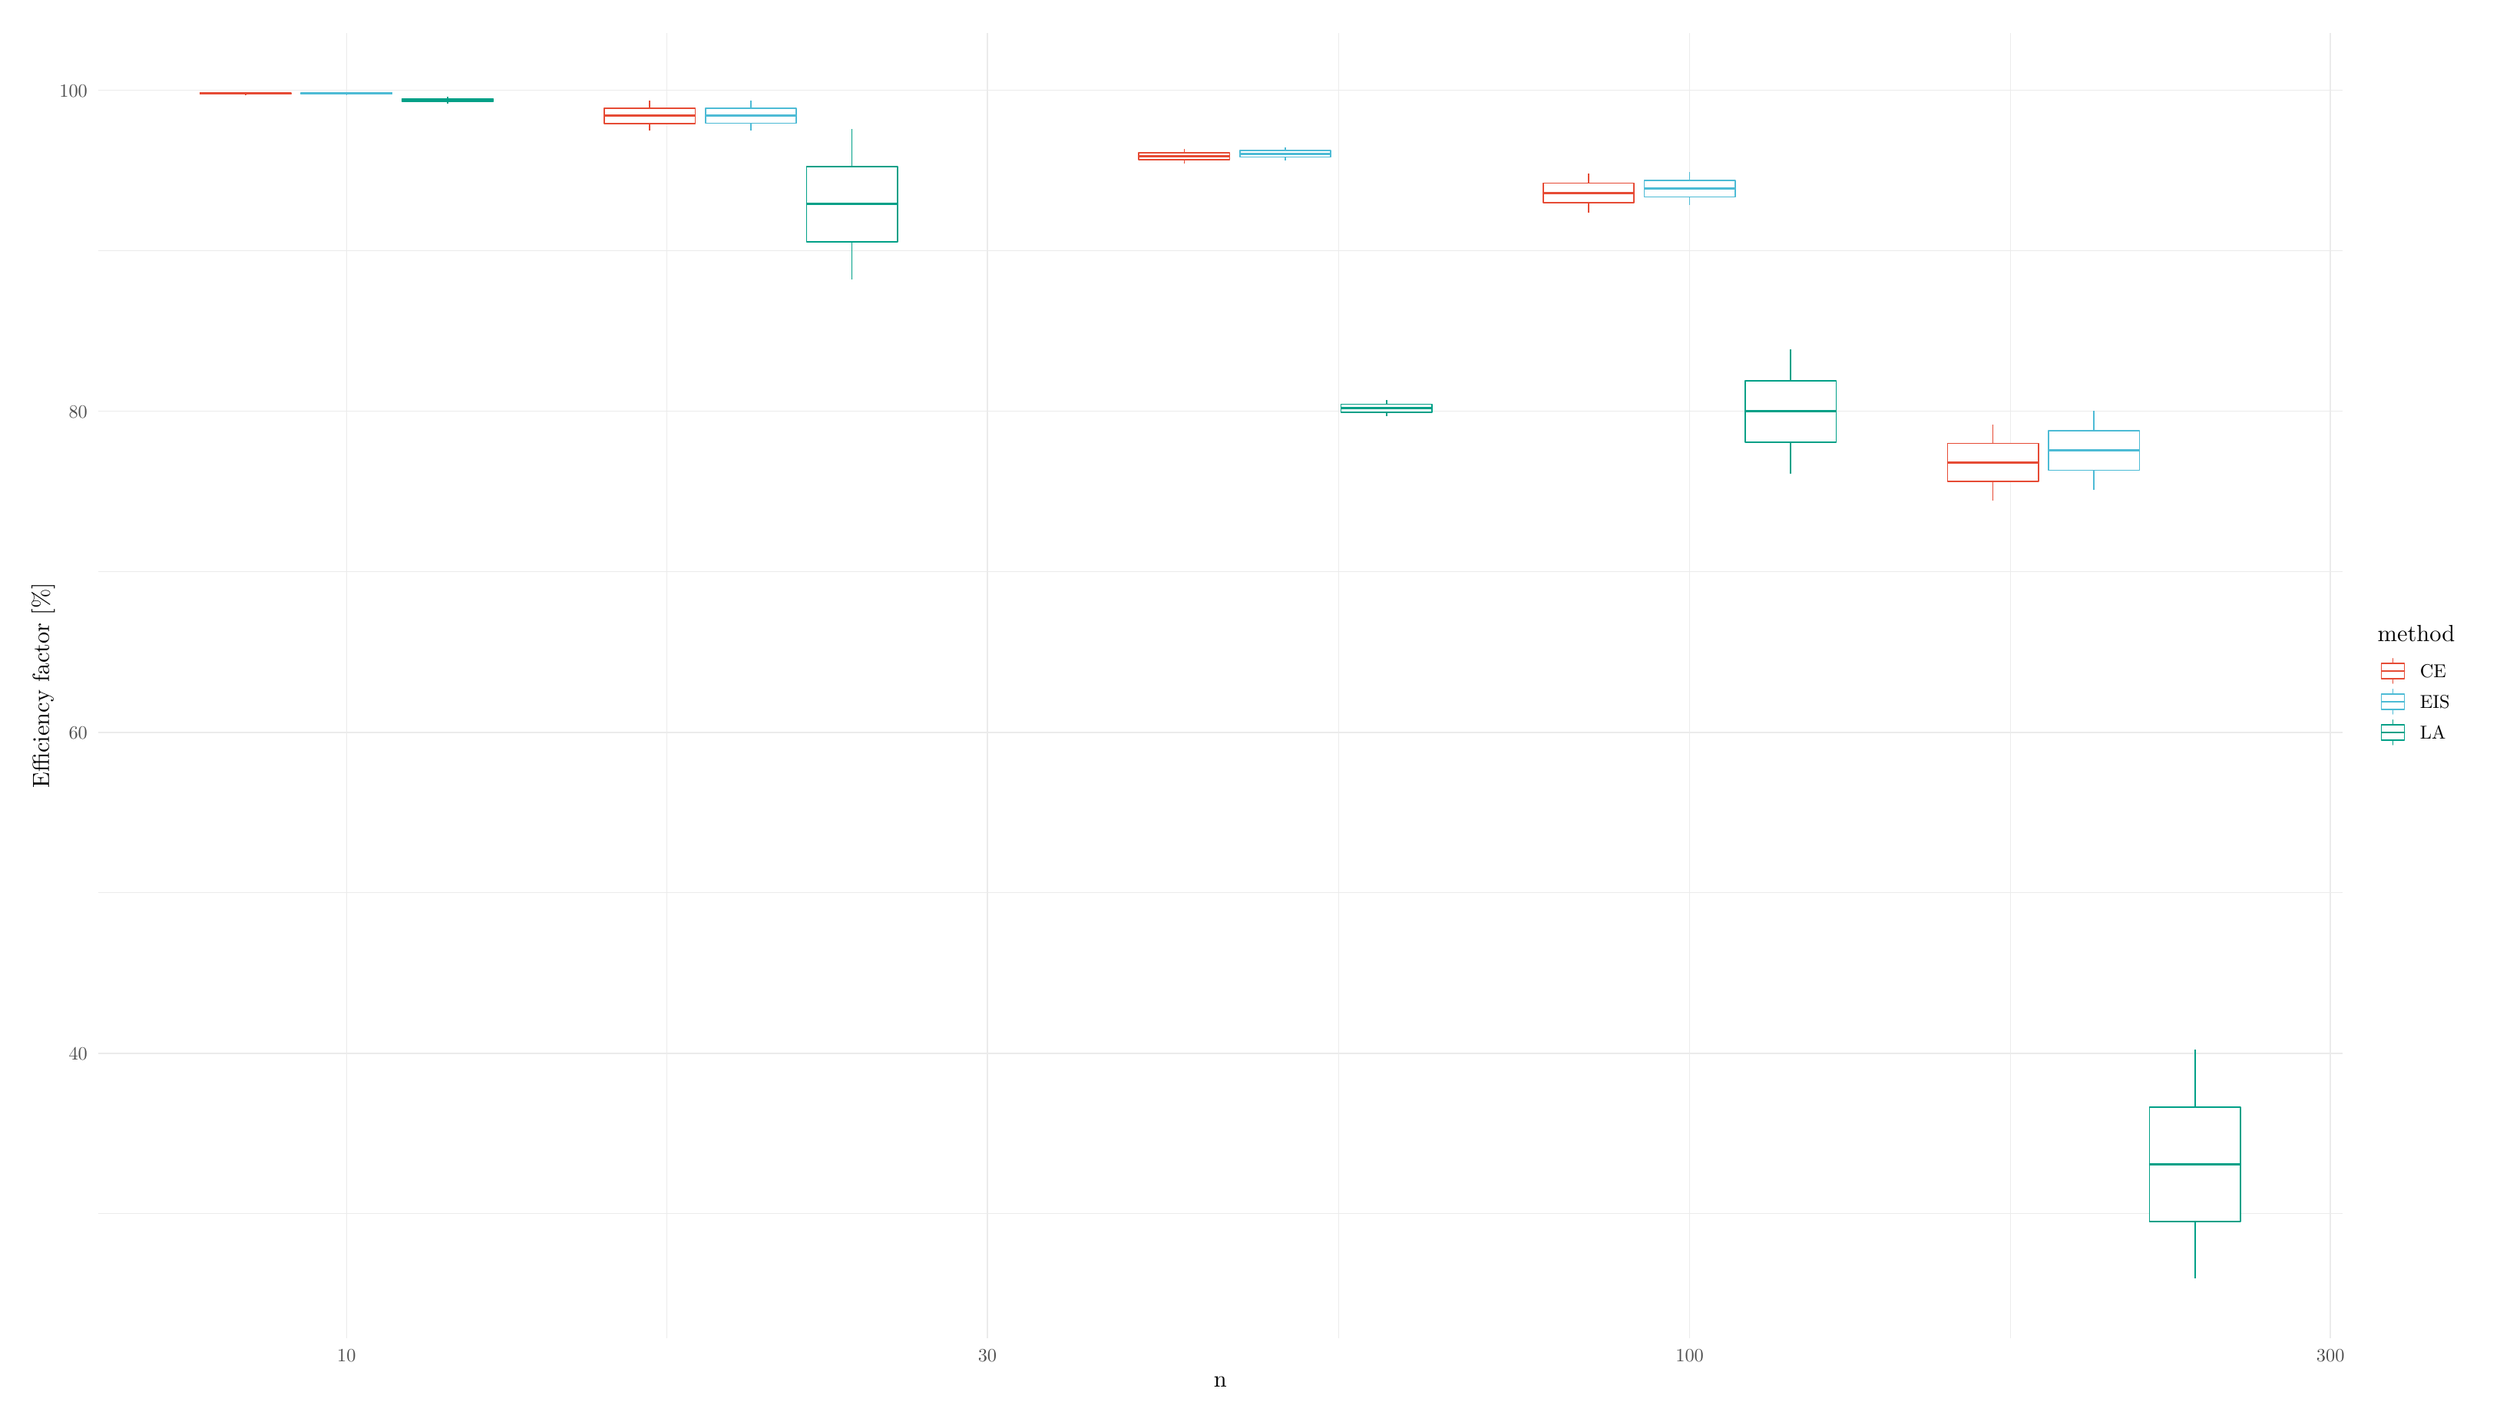
\begin{tikzpicture}[x=1pt,y=1pt]
\definecolor{fillColor}{RGB}{255,255,255}
\path[use as bounding box,fill=fillColor,fill opacity=0.00] (0,0) rectangle (1156.32,650.43);
\begin{scope}
\path[clip] ( 36.11, 30.69) rectangle (1092.47,644.93);
\definecolor{drawColor}{gray}{0.92}

\path[draw=drawColor,line width= 0.3pt,line join=round] ( 36.11, 89.19) --
	(1092.47, 89.19);

\path[draw=drawColor,line width= 0.3pt,line join=round] ( 36.11,240.26) --
	(1092.47,240.26);

\path[draw=drawColor,line width= 0.3pt,line join=round] ( 36.11,391.33) --
	(1092.47,391.33);

\path[draw=drawColor,line width= 0.3pt,line join=round] ( 36.11,542.40) --
	(1092.47,542.40);

\path[draw=drawColor,line width= 0.3pt,line join=round] (303.90, 30.69) --
	(303.90,644.93);

\path[draw=drawColor,line width= 0.3pt,line join=round] (619.94, 30.69) --
	(619.94,644.93);

\path[draw=drawColor,line width= 0.3pt,line join=round] (935.99, 30.69) --
	(935.99,644.93);

\path[draw=drawColor,line width= 0.6pt,line join=round] ( 36.11,164.72) --
	(1092.47,164.72);

\path[draw=drawColor,line width= 0.6pt,line join=round] ( 36.11,315.79) --
	(1092.47,315.79);

\path[draw=drawColor,line width= 0.6pt,line join=round] ( 36.11,466.86) --
	(1092.47,466.86);

\path[draw=drawColor,line width= 0.6pt,line join=round] ( 36.11,617.93) --
	(1092.47,617.93);

\path[draw=drawColor,line width= 0.6pt,line join=round] (153.10, 30.69) --
	(153.10,644.93);

\path[draw=drawColor,line width= 0.6pt,line join=round] (454.69, 30.69) --
	(454.69,644.93);

\path[draw=drawColor,line width= 0.6pt,line join=round] (785.20, 30.69) --
	(785.20,644.93);

\path[draw=drawColor,line width= 0.6pt,line join=round] (1086.78, 30.69) --
	(1086.78,644.93);
\definecolor{drawColor}{RGB}{230,75,53}

\path[draw=drawColor,line width= 0.6pt,line join=round] (105.53,616.69) -- (105.53,616.99);

\path[draw=drawColor,line width= 0.6pt,line join=round] (105.53,616.10) -- (105.53,615.80);
\definecolor{fillColor}{RGB}{255,255,255}

\path[draw=drawColor,line width= 0.6pt,line join=round,line cap=round,fill=fillColor] ( 84.13,616.69) --
	( 84.13,616.10) --
	(126.94,616.10) --
	(126.94,616.69) --
	( 84.13,616.69) --
	cycle;

\path[draw=drawColor,line width= 1.1pt,line join=round] ( 84.13,616.39) -- (126.94,616.39);

\path[draw=drawColor,line width= 0.6pt,line join=round] (295.81,609.43) -- (295.81,612.96);

\path[draw=drawColor,line width= 0.6pt,line join=round] (295.81,602.35) -- (295.81,598.82);

\path[draw=drawColor,line width= 0.6pt,line join=round,line cap=round,fill=fillColor] (274.41,609.43) --
	(274.41,602.35) --
	(317.22,602.35) --
	(317.22,609.43) --
	(274.41,609.43) --
	cycle;

\path[draw=drawColor,line width= 1.1pt,line join=round] (274.41,605.89) -- (317.22,605.89);

\path[draw=drawColor,line width= 0.6pt,line join=round] (547.35,588.56) -- (547.35,590.26);

\path[draw=drawColor,line width= 0.6pt,line join=round] (547.35,585.16) -- (547.35,583.46);

\path[draw=drawColor,line width= 0.6pt,line join=round,line cap=round,fill=fillColor] (525.94,588.56) --
	(525.94,585.16) --
	(568.75,585.16) --
	(568.75,588.56) --
	(525.94,588.56) --
	cycle;

\path[draw=drawColor,line width= 1.1pt,line join=round] (525.94,586.86) -- (568.75,586.86);

\path[draw=drawColor,line width= 0.6pt,line join=round] (737.63,574.25) -- (737.63,578.85);

\path[draw=drawColor,line width= 0.6pt,line join=round] (737.63,565.05) -- (737.63,560.45);

\path[draw=drawColor,line width= 0.6pt,line join=round,line cap=round,fill=fillColor] (716.22,574.25) --
	(716.22,565.05) --
	(759.03,565.05) --
	(759.03,574.25) --
	(716.22,574.25) --
	cycle;

\path[draw=drawColor,line width= 1.1pt,line join=round] (716.22,569.65) -- (759.03,569.65);

\path[draw=drawColor,line width= 0.6pt,line join=round] (927.91,451.78) -- (927.91,460.73);

\path[draw=drawColor,line width= 0.6pt,line join=round] (927.91,433.88) -- (927.91,424.94);

\path[draw=drawColor,line width= 0.6pt,line join=round,line cap=round,fill=fillColor] (906.50,451.78) --
	(906.50,433.88) --
	(949.31,433.88) --
	(949.31,451.78) --
	(906.50,451.78) --
	cycle;

\path[draw=drawColor,line width= 1.1pt,line join=round] (906.50,442.83) -- (949.31,442.83);
\definecolor{drawColor}{RGB}{77,187,213}

\path[draw=drawColor,line width= 0.6pt,line join=round] (153.10,616.72) -- (153.10,617.01);

\path[draw=drawColor,line width= 0.6pt,line join=round] (153.10,616.15) -- (153.10,615.86);

\path[draw=drawColor,line width= 0.6pt,line join=round,line cap=round,fill=fillColor] (131.70,616.72) --
	(131.70,616.15) --
	(174.51,616.15) --
	(174.51,616.72) --
	(131.70,616.72) --
	cycle;

\path[draw=drawColor,line width= 1.1pt,line join=round] (131.70,616.44) -- (174.51,616.44);

\path[draw=drawColor,line width= 0.6pt,line join=round] (343.38,609.50) -- (343.38,613.04);

\path[draw=drawColor,line width= 0.6pt,line join=round] (343.38,602.43) -- (343.38,598.90);

\path[draw=drawColor,line width= 0.6pt,line join=round,line cap=round,fill=fillColor] (321.98,609.50) --
	(321.98,602.43) --
	(364.79,602.43) --
	(364.79,609.50) --
	(321.98,609.50) --
	cycle;

\path[draw=drawColor,line width= 1.1pt,line join=round] (321.98,605.97) -- (364.79,605.97);

\path[draw=drawColor,line width= 0.6pt,line join=round] (594.92,589.52) -- (594.92,591.02);

\path[draw=drawColor,line width= 0.6pt,line join=round] (594.92,586.50) -- (594.92,584.99);

\path[draw=drawColor,line width= 0.6pt,line join=round,line cap=round,fill=fillColor] (573.51,589.52) --
	(573.51,586.50) --
	(616.32,586.50) --
	(616.32,589.52) --
	(573.51,589.52) --
	cycle;

\path[draw=drawColor,line width= 1.1pt,line join=round] (573.51,588.01) -- (616.32,588.01);

\path[draw=drawColor,line width= 0.6pt,line join=round] (785.20,575.56) -- (785.20,579.45);

\path[draw=drawColor,line width= 0.6pt,line join=round] (785.20,567.77) -- (785.20,563.88);

\path[draw=drawColor,line width= 0.6pt,line join=round,line cap=round,fill=fillColor] (763.79,575.56) --
	(763.79,567.77) --
	(806.60,567.77) --
	(806.60,575.56) --
	(763.79,575.56) --
	cycle;

\path[draw=drawColor,line width= 1.1pt,line join=round] (763.79,571.66) -- (806.60,571.66);

\path[draw=drawColor,line width= 0.6pt,line join=round] (975.48,457.70) -- (975.48,467.03);

\path[draw=drawColor,line width= 0.6pt,line join=round] (975.48,439.05) -- (975.48,429.72);

\path[draw=drawColor,line width= 0.6pt,line join=round,line cap=round,fill=fillColor] (954.07,457.70) --
	(954.07,439.05) --
	(996.88,439.05) --
	(996.88,457.70) --
	(954.07,457.70) --
	cycle;

\path[draw=drawColor,line width= 1.1pt,line join=round] (954.07,448.38) -- (996.88,448.38);
\definecolor{drawColor}{RGB}{0,160,135}

\path[draw=drawColor,line width= 0.6pt,line join=round] (200.67,614.00) -- (200.67,614.74);

\path[draw=drawColor,line width= 0.6pt,line join=round] (200.67,612.51) -- (200.67,611.77);

\path[draw=drawColor,line width= 0.6pt,line join=round,line cap=round,fill=fillColor] (179.27,614.00) --
	(179.27,612.51) --
	(222.08,612.51) --
	(222.08,614.00) --
	(179.27,614.00) --
	cycle;

\path[draw=drawColor,line width= 1.1pt,line join=round] (179.27,613.26) -- (222.08,613.26);

\path[draw=drawColor,line width= 0.6pt,line join=round] (390.95,582.03) -- (390.95,599.71);

\path[draw=drawColor,line width= 0.6pt,line join=round] (390.95,546.68) -- (390.95,529.00);

\path[draw=drawColor,line width= 0.6pt,line join=round,line cap=round,fill=fillColor] (369.55,582.03) --
	(369.55,546.68) --
	(412.36,546.68) --
	(412.36,582.03) --
	(369.55,582.03) --
	cycle;

\path[draw=drawColor,line width= 1.1pt,line join=round] (369.55,564.36) -- (412.36,564.36);

\path[draw=drawColor,line width= 0.6pt,line join=round] (642.49,470.16) -- (642.49,472.06);

\path[draw=drawColor,line width= 0.6pt,line join=round] (642.49,466.37) -- (642.49,464.48);

\path[draw=drawColor,line width= 0.6pt,line join=round,line cap=round,fill=fillColor] (621.08,470.16) --
	(621.08,466.37) --
	(663.89,466.37) --
	(663.89,470.16) --
	(621.08,470.16) --
	cycle;

\path[draw=drawColor,line width= 1.1pt,line join=round] (621.08,468.27) -- (663.89,468.27);

\path[draw=drawColor,line width= 0.6pt,line join=round] (832.77,481.29) -- (832.77,495.84);

\path[draw=drawColor,line width= 0.6pt,line join=round] (832.77,452.20) -- (832.77,437.65);

\path[draw=drawColor,line width= 0.6pt,line join=round,line cap=round,fill=fillColor] (811.36,481.29) --
	(811.36,452.20) --
	(854.17,452.20) --
	(854.17,481.29) --
	(811.36,481.29) --
	cycle;

\path[draw=drawColor,line width= 1.1pt,line join=round] (811.36,466.75) -- (854.17,466.75);

\path[draw=drawColor,line width= 0.6pt,line join=round] (1023.04,139.43) -- (1023.04,166.37);

\path[draw=drawColor,line width= 0.6pt,line join=round] (1023.04, 85.55) -- (1023.04, 58.61);

\path[draw=drawColor,line width= 0.6pt,line join=round,line cap=round,fill=fillColor] (1001.64,139.43) --
	(1001.64, 85.55) --
	(1044.45, 85.55) --
	(1044.45,139.43) --
	(1001.64,139.43) --
	cycle;

\path[draw=drawColor,line width= 1.1pt,line join=round] (1001.64,112.49) -- (1044.45,112.49);
\end{scope}
\begin{scope}
\path[clip] (  0.00,  0.00) rectangle (1156.32,650.43);
\definecolor{drawColor}{gray}{0.30}

\node[text=drawColor,anchor=base east,inner sep=0pt, outer sep=0pt, scale=  0.88] at ( 31.16,161.69) {40};

\node[text=drawColor,anchor=base east,inner sep=0pt, outer sep=0pt, scale=  0.88] at ( 31.16,312.76) {60};

\node[text=drawColor,anchor=base east,inner sep=0pt, outer sep=0pt, scale=  0.88] at ( 31.16,463.83) {80};

\node[text=drawColor,anchor=base east,inner sep=0pt, outer sep=0pt, scale=  0.88] at ( 31.16,614.90) {100};
\end{scope}
\begin{scope}
\path[clip] (  0.00,  0.00) rectangle (1156.32,650.43);
\definecolor{drawColor}{gray}{0.30}

\node[text=drawColor,anchor=base,inner sep=0pt, outer sep=0pt, scale=  0.88] at (153.10, 19.68) {10};

\node[text=drawColor,anchor=base,inner sep=0pt, outer sep=0pt, scale=  0.88] at (454.69, 19.68) {30};

\node[text=drawColor,anchor=base,inner sep=0pt, outer sep=0pt, scale=  0.88] at (785.20, 19.68) {100};

\node[text=drawColor,anchor=base,inner sep=0pt, outer sep=0pt, scale=  0.88] at (1086.78, 19.68) {300};
\end{scope}
\begin{scope}
\path[clip] (  0.00,  0.00) rectangle (1156.32,650.43);
\definecolor{drawColor}{RGB}{0,0,0}

\node[text=drawColor,anchor=base,inner sep=0pt, outer sep=0pt, scale=  1.10] at (564.29,  7.64) {n};
\end{scope}
\begin{scope}
\path[clip] (  0.00,  0.00) rectangle (1156.32,650.43);
\definecolor{drawColor}{RGB}{0,0,0}

\node[text=drawColor,rotate= 90.00,anchor=base,inner sep=0pt, outer sep=0pt, scale=  1.10] at ( 13.08,337.81) {Efficiency factor [\%]};
\end{scope}
\begin{scope}
\path[clip] (  0.00,  0.00) rectangle (1156.32,650.43);
\definecolor{drawColor}{RGB}{0,0,0}

\node[text=drawColor,anchor=base west,inner sep=0pt, outer sep=0pt, scale=  1.10] at (1108.97,358.45) {method};
\end{scope}
\begin{scope}
\path[clip] (  0.00,  0.00) rectangle (1156.32,650.43);
\definecolor{drawColor}{RGB}{230,75,53}

\path[draw=drawColor,line width= 0.6pt,line join=round,line cap=round] (1116.19,338.87) --
	(1116.19,341.04);

\path[draw=drawColor,line width= 0.6pt,line join=round,line cap=round] (1116.19,348.27) --
	(1116.19,350.44);
\definecolor{fillColor}{RGB}{255,255,255}

\path[draw=drawColor,line width= 0.6pt,line join=round,line cap=round,fill=fillColor] (1110.77,341.04) rectangle (1121.61,348.27);

\path[draw=drawColor,line width= 0.6pt,line join=round,line cap=round] (1110.77,344.65) --
	(1121.61,344.65);
\end{scope}
\begin{scope}
\path[clip] (  0.00,  0.00) rectangle (1156.32,650.43);
\definecolor{drawColor}{RGB}{77,187,213}

\path[draw=drawColor,line width= 0.6pt,line join=round,line cap=round] (1116.19,324.42) --
	(1116.19,326.59);

\path[draw=drawColor,line width= 0.6pt,line join=round,line cap=round] (1116.19,333.81) --
	(1116.19,335.98);
\definecolor{fillColor}{RGB}{255,255,255}

\path[draw=drawColor,line width= 0.6pt,line join=round,line cap=round,fill=fillColor] (1110.77,326.59) rectangle (1121.61,333.81);

\path[draw=drawColor,line width= 0.6pt,line join=round,line cap=round] (1110.77,330.20) --
	(1121.61,330.20);
\end{scope}
\begin{scope}
\path[clip] (  0.00,  0.00) rectangle (1156.32,650.43);
\definecolor{drawColor}{RGB}{0,160,135}

\path[draw=drawColor,line width= 0.6pt,line join=round,line cap=round] (1116.19,309.97) --
	(1116.19,312.13);

\path[draw=drawColor,line width= 0.6pt,line join=round,line cap=round] (1116.19,319.36) --
	(1116.19,321.53);
\definecolor{fillColor}{RGB}{255,255,255}

\path[draw=drawColor,line width= 0.6pt,line join=round,line cap=round,fill=fillColor] (1110.77,312.13) rectangle (1121.61,319.36);

\path[draw=drawColor,line width= 0.6pt,line join=round,line cap=round] (1110.77,315.75) --
	(1121.61,315.75);
\end{scope}
\begin{scope}
\path[clip] (  0.00,  0.00) rectangle (1156.32,650.43);
\definecolor{drawColor}{RGB}{0,0,0}

\node[text=drawColor,anchor=base west,inner sep=0pt, outer sep=0pt, scale=  0.88] at (1128.92,341.62) {CE};
\end{scope}
\begin{scope}
\path[clip] (  0.00,  0.00) rectangle (1156.32,650.43);
\definecolor{drawColor}{RGB}{0,0,0}

\node[text=drawColor,anchor=base west,inner sep=0pt, outer sep=0pt, scale=  0.88] at (1128.92,327.17) {EIS};
\end{scope}
\begin{scope}
\path[clip] (  0.00,  0.00) rectangle (1156.32,650.43);
\definecolor{drawColor}{RGB}{0,0,0}

\node[text=drawColor,anchor=base west,inner sep=0pt, outer sep=0pt, scale=  0.88] at (1128.92,312.72) {LA};
\end{scope}
\end{tikzpicture}
%
    }
    \caption{The efficiency factor degenerates as the number of time steps $n$ increases. We show the estimated efficiency factor over $100$ replications of estimating the optimal parameters for \Cref{ex:negbinom-ar1} with the \gls{cem} and \gls{eis} with $N_{\text{true}} = 10^{6}$ and the resulting estimated efficiency factors at the optimum. Notice the log scale of the x-axis. The performance of the optimal \gls{cem} and \gls{eis} parameters is comparable and superior to that of the \gls{la}}
    \label{fig:ef_time_dimension}
\end{figure}


\subsection{Breakdown of methods}

\subsection{Optimal parameters}

\begin{example}[Failure of \gls{la}]
  \label{ex:la_failure}
  Consider the Gaussian scale mixture $\P = \frac{1}{2} \left(\mathcal N (0,1) + \mathcal N(0, \varepsilon^{-2})\right)$ with mode $x^{\ast}=0$. 
  The \gls{la} is $\G_{\text{LA}} = \mathcal N \left( 0, \frac{1}{\varepsilon^{2} - \varepsilon + 1} \right)$, whose variance goes to $1$ as $\varepsilon$ goes to $0$, so the \gls{la} will miss close to $\frac 1 2$ of the total mass.
  For $\varepsilon$ small enough, the variance of the \gls{la} will be smaller than $\frac{1}{2\varepsilon^{2}}$, whence the second moment of the weights is infinite and importance sampling fails.

  The \gls{cem} minimizes the KL-divergence between $\P$ and $\G_{\psi}$, is given by $\G_{\text{CE}} = \mathcal N (0, \sigma^{2})$, where $\sigma^{2} = \frac{1}{2}\left( 1 + \varepsilon^{-2} \right)$ is the variance of $\P$.
  As $\sigma^{2} > \frac{1}{2}\varepsilon^{-2}$, the weights have finite second moment, and importance sampling is consistent.
  \todo{add proof for $\frac{1}{2}$ to appendix}
\end{example}

\subsection{Time complexity}

\subsection{Large sample behaviour}

\begin{itemize}
    \item stationary AR(1) process with high auto-correlation, NB observations, different $n$, large $N$, compare ESS, Variances, DKL(?)
\end{itemize}